\documentclass[abstracton]{scrreprt}
\usepackage{amssymb}
\usepackage{mathtools}
\usepackage{dsfont}
\usepackage{scrhack}
\usepackage{graphicx}
\usepackage{caption}
\usepackage{subcaption}
\usepackage{pgfplots}
\usepackage{listings}
\usepackage{xcolor}
\usepackage{framed}
\usepackage{url}
\usepackage{setspace}
\usepackage[english]{babel}
\usepackage[utf8]{inputenc}
\usepackage[automark,headsepline]{scrlayer-scrpage}

\clearpairofpagestyles
\cfoot[\pagemark]{\pagemark}
\lehead{\headmark}
\rohead{\headmark}
\pagestyle{scrheadings}

\lstset { %
    language=C++,
    backgroundcolor=\color{black!5}, % set backgroundcolor
    basicstyle=\footnotesize,% basic font setting
    frame=single, % adds a frame around the code
    breaklines=true, % sets automatic line breaking
}

\pgfplotsset{compat=1.12}
\pgfplotsset{soldot/.style={color=blue,only marks,mark=*}}
\pgfplotsset{holdot/.style={color=blue,fill=white,only marks,mark=*}}

% Set counter for section
\setcounter{section}{1}
\setcounter{subsection}{1}
\setcounter{tocdepth}{1}
\setlength{\parindent}{0pt}

% new commands
\newcommand{\qed}{$\hfill\blacksquare$}
% new commands (end)

% new theorems
\newtheorem{theorem}{Theorem}[chapter]
\newtheorem{lemma}[theorem]{Lemma}
\newtheorem{proposition}[theorem]{Proposition}
\newtheorem{corollary}[theorem]{Corollary}
\newtheorem{definition}[theorem]{Definition}
\newtheorem{example}[theorem]{Example}
\newtheorem{remark}[theorem]{Remark}
\newtheorem{algorithm}[theorem]{Algorithm}
% new theorems (end)

% new environments
\newenvironment{proof}[1][Proof]{\begin{trivlist}
\item[\hskip \labelsep {\bfseries #1}]}{\end{trivlist}}
\newenvironment{describe}[1][]{\begin{trivlist}
\item[\hskip \labelsep {\bfseries #1}]\itshape}{\end{trivlist}}
% new environments (end)

\begin{document}

\pagenumbering{Roman} % set page numbering to Roman

% title_page
\begin{titlepage} % (fold)
    \begin{center}
        \begin{large}
            \textsc{Universit\"at Regensburg\\
                Fakult\"at f\"ur Mathematik\\
            }
        \end{large}
        \vspace{0.5cm}
        \begin{huge}
            \begin{spacing}{0.9}
            \textsc{Solving Convex and Non-Convex Functionals in Image Processing using a Primal-Dual Algorithm}
            \end{spacing}
        \end{huge}
        \vspace{1.2cm}
        \begin{center}
        
\includegraphics[width=7.5cm]{img/sigillum.png}
        \vspace{1.0cm}\\
        \begin{Large}
            \textsc{Masterarbeit}\\
        \end{Large}
        \vspace{0.5cm}
        \begin{large}
            \textsc{zur Erlangung des akademischen Grades\\
                Master of Science\\
                im Studiengang Computational Science\\
                \vspace{0.5cm}
                Eingereicht bei Prof. Dr. Harald Garcke\\
                am 17.03.2016\\
            }
        \end{large}
        \vspace{1.0cm}
    \end{center}

    \begin{flushleft}
        \begin{large}
            \textsc{Vorgelegt von:\\
                Michael Bauer\\
                Geboren am 23. August 1987 in Gr\"afelfing\\
                Matrikelnummer 152 8558
            }
        \end{large}
    \end{flushleft}
    \end{center}
\end{titlepage}
% title_page (end)

\newpage
\thispagestyle{empty}
\mbox{}

\renewcommand\abstractname{Acknowledgements}
\begin{abstract}
    This thesis is the last part of my degree course Computational Science which I could never have done without the support of several people. Now, I get the chance to thank everybody who contributed directly or indirectly and gave me assistance, whenever I needed it.\\
    
    For being patient, supportive, motivating and always positive I have to thank you so much Sylvia Wallner. Also lot of thanks to my mother for your patience and support. For fruitful discussions, listening to all my presentations at least once and correcting silly mistakes I want to thank Leonie Jennert and Bernhard Zimmermann. Thank you Michael Huttner for the great discussions about programming and your help.\\
    
    The basis of this thesis are works published by Prof. Dr. Daniel Cremers (TUM). Thanks to you and your group, especially Thomas Moellenhoff, for the chance to join the CUDA course and for your external contribution to this work.\\
    
    The thesis itself was written at the chair of Prof. Dr. Harald Garcke, who also supervised me. So, last but not least I want to thank you so much for your input, your support and your constructive criticism. Our discussions always brought me one step further and let me see each problem from another point of view.\\
\end{abstract}

\newpage
\thispagestyle{empty}
\mbox{}

\renewcommand\abstractname{Abstract}

\begin{abstract}
    In this thesis we consider three different functionals in image processing. Our goal is to minimze the energy of each functional to approximate an input image optimally. By solving these optimization problems we derive applications to imaging like image cartooning, denoising, inpainting and segmentation.\\
    
    The algorithm which computes the minimal energy of each functional is a primal-dual algorithm. This framework solves saddle-point problems and is highly parallelizable. In order to be able to apply the algorithm we turn all our minimization into saddle-point problems. One convex functional we consider is the so called ROF functional, first proposed by Rudin, Osher and Fatemi, hence the name. It is based on a least squares and a total variation term. Using the total variation together with a term based on the L1 norm we derive the convex TVL1 functional which we also consider in this work.\\
    
    Even though, the third functional, namely the Mumford-Shah functional, is non-convex we use convex analysis to turn the minimization of the functional into a saddle-point problem. This strategy does not lead to a provable minimal value of the Mumford-Shah functional, but we get high-quality approximations of images. Additionally, we consider a second approach for minimizing the non-convex Mumford-Shah functional. We make use of convex relaxation techniques to turn the minimization into a convex saddle-point problem. Then, we apply again the primal-dual algorithm to solve this optimization problem.\\

    In terms of the convex relaxed functional the primal-dual algorithm has a bad performance. This is related to Dykstra's projection algorithm which is used in each iteration step of the primal-dual algorithm. To resolve the run-time issue we present a method for solving the convex relaxed Mumford-Shah model using Lagrange multipliers. We show that this approach creates a tremendous performance increase. In the case of the other three frameworks we demonstrate that the primal-dual algorithm has real-time applicability.\\
    
    Finally, we present image cartooning and a comparison for image denoising with the proposed models. A modified version of the ROF functional is taken into account when we present image inpainting and at last we show that the Mumford-Shah functional fits perfectly for image segmentation.
\end{abstract}

% Content, Tables, Figures
\tableofcontents
% \listoftables
% \listoffigures
% Content, Tables, Figures (end)

\pagenumbering{arabic} % set page numbering back to arabic

\chapter{Introduction} % (fold)
\label{cha:introduction}
    In the second decade of the twenty-first century autonomous driving seems to be an important thing for the car, computer and software industry. The expectation is nothing less than having fewer, or even no, accidents. With these cars, industry is trying to change the world for a better. As this may comfort many people, it poses a lot of technical and computational issues, for instance a stable hardware or even more important viable software. One field of research - of many others - is called Machine Learning, where the computer is trained to make the right decisions in the right situations. The car should be able to accommodate to all possible circumstances which could appear during a drive. To make it even more complicated, the onboard computer needs to decide in real-time. As one can imagine, it is extremely difficult to develop fast, stable and tractable computer programs.\\
    In order to learn from a certain situation the computer needs data from the environment. This can be the shape of another car, traffic lights, differences in the lighting conditions or the distance to other objects. What all these information have in common: They can be collected via images. Small cameras are tracking the traffic and surrounding and providing the necessary data for the software. But it is not only the autonomously driving car which makes use of images. Doctors use X-ray view or MRI scans in patient treatment and semiconductor companies use pictures of wafers looking for damages on it, for example scratches or dark spots. For this reason, image processing has become more important during the last decades. Researchers dealt with many problems like edge detection, deblurring, denoising, inpainting or image segmentation. In the field of edge detection the probably most famous researcher is John F. Canny. He presented a stable edge detection algorithm in 1986 (cf. \cite{Canny}), also known as Canny-Edge-Detector.\\
    Only three years after Canny published his work, two researchers, namely David Mumford and Jayant Shah, published a paper (\cite{Mumford-et-al-cpam}), whose impact is still present. According to Google Scholar their publication was cited over 4.703 times, as of March 12th 2016. They suggested to minimize the energy of the so called Mumford-Shah functional in order to approximate an input image optimally. Solving this optimization problem leads to applications like image denoising, inpainting and segmentation. Unfortunately, this functional is by definition non-convex. For this reason finding the minimal energy of it is a hard task.\\
    One approach for minimizing the Mumford-Shah functional was published in 2009 by Pock, Cremers, Bischof and Chambolle in \cite{Pock-et-al-iccv09}. We consider this approach in this thesis and present an alternative approach to their proposed method using a Lagrange multiplier formalism. This will lead us to a tremendous performance increase compared to the original suggested framework. Pock et al. also proposed a novel primal-dual algorithm in \cite{Pock-et-al-iccv09} in order to compute the minimizer of the functional. The algorithm itself is a solver for saddle-point problems and highly parallelizable. In 2011 Pock and Chambolle published a work (\cite{Chambolle10afirst-order}), cited 1.234 times (Google Scholar) as of March 12th 2016, in which they generalized the primal-dual algorithm and showed applications to imaging with it. So, this framework has grown to a powerful tool in the last years to solve saddle-point problems efficiently.\\
    One functional Pock and Chambolle consider in their work of 2011 is the ROF functional. It was proposed in 1992 by the researchers Rudin, Osher and Fatemi (\cite{ROF}). They suggested to minimize the energy of this convex functional. The functional itself involves a least squares data term and uses the total variation as regularizer term. By replacing the norm of the least squares data term in the ROF functional with the L1 norm one derives the convex TVL1 functional. Minimizing these two convex functionals can efficiently be done by using techniques of convex analysis. By applying convex analysis we turn the minimization of the functionals into saddle-point problems, for which we can use the primal-dual algorithm as a solver. Further, we discuss an approach to the Mumford-Shah functional which proceeds in the same fashion as for minimizing the ROF and TVL1 functional. In 2014 Strekalovskiy and Cremers used convex analysis in order to minimize the non-convex Mumford-Shah functional. Even though, this strategy does not lead to a provable minimal value of the optimization problem, we show that we derive high-quality image approximations with this formulation.\\
    In this work we introduce the three functionals, namely ROF, TVL1 and Mumford-Shah, the total variation and concepts of convex analysis. After providing the frameworks for minimizing the functionals we estimate applicable parameters used in the models and present applications to imaging. Whereas cartooning and denoising are impressive applications, image inpainting and image segmentation are really imposing.
% chapter introduction (end)

\chapter{Basic Concepts} % (fold)
\label{cha:basic_concepts}

    In this chapter we give an introduction to the most important concepts we meet in this thesis. We start by defining images in a mathematical manner, then introduce basic concepts of convex analysis and the total variation.
    \section{Images in Mathematics} % (fold)
    \label{sec:images_in_mathematics}

        Images can be viewed as mathematical objects. We can distinguish between discrete and continuous images. Let us first introduce images in the mathematical sense and then give some examples. The definition and examples can be found in the work of Kristian Bredies and Dirk Lorenz \cite{Bredies}.

        \begin{definition}[Image] % (fold)
        \label{def:image}
            Let $\Omega \subseteq \mathbb{R}^{n}$ be an image domain and $C$ be a color space. An n-dimensional image $u$ is a mapping $u: \Omega \longrightarrow C$, where each point in $\Omega$ corresponds to a color value in $C$.
        \end{definition}
        % definition image (end)
        \begin{remark}[Continuous and discrete images] % (fold)
        \label{rem:continuous_vs_discrete}
            Images can be discrete or continuous. The difference between these two classes is determined in the image domain $\Omega$.
                \begin{itemize}
                    \item Let $\Omega = \{ 1, ..., N \}^{n}$, then $u$ is a discrete image, since $\Omega$ is a discrete set. All images on computers are discrete, because each single pixel lies at a fixed, discrete position $(i,j)$.
                    \item Let $\Omega \subseteq \mathbb{R}^{n}$, then $u$ is a continuous image. For instance, we could set $\Omega = [a, b]^{n}$ with $a, b \in \mathbb{R}$ and $a < b$.
                \end{itemize}
            There are several image types, like binary or colored images. The property, to which type an image $u$ belongs, is determined by the color space $C$:
                \begin{itemize}
                    \item Let $C = \{ 0, 1 \}$, then we call $u$ binary or black-and-white image.
                    \item In the case of grayscaled images we set $C = \{ 0, ..., 2^{k}-1 \}$, where the value $k$ determines the bit depth. Usually, we find $k = 8$ in computers, i.e. grayscaled images take on values in between $0$ and $255$, where $0 = \textnormal{black}$ and $255 = \textnormal{white}$.
                    \item A n-dimensional color image has $C = \{ 0, ..., 2^{k}-1 \}^{n}$, for instance $n = 3$ for RGB (red-green-blue) images.
                    \item An image $u$ could also map to continuous color spaces, e.g. $C = [a, b]^{n}$ or $C = \mathbb{R}^{n}$. Most common are RGB images with $n = 3$, $a = 0$ and $b = 1$.
                \end{itemize}
        \end{remark}
        % remark continuous_vs_discrete (end)
        In this thesis we consider two discrete settings for the domain $\Omega$. One where $\Omega$ is two-dimensional, and the other where $\Omega$ is a three-dimensional space. In the first case, we call a point $(i, j)$ in $\Omega$ pixel, in the second a point $(i, j, k)$ is called voxel.
        \begin{figure}[!ht]
            \centering
                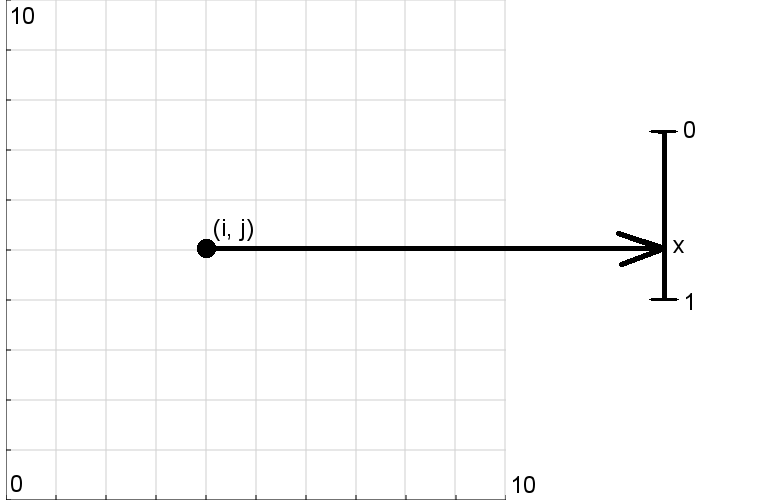
\includegraphics[width=0.6\textwidth]{img/image_mapping.png}
            \caption[Mapping of images.]{An image function $u: \{0,1,...,10\}^{2} \to [0,1]$, mapping a pixel $(i,j)$ to the value $x \in [0,1]$.}
        \label{fig:image_mapping}
        \end{figure}
    % section images_in_mathematics (end)
    \section{Convex Optimization and Convex Analysis} % (fold)
    \label{sec:convex_optimization_and_convex_analysis}

        In this section we cover some topics which are related to convex analysis. Since we are facing (convex) optimization problems, we first define this class of programs. We follow with our notations, definitions and theorems the book of Nocedal and Wright (\cite{Nocedal-Wright}). An optimization problem is given by
            \begin{equation} % (fold)
                \min_{x \in \mathbb{R}^{n}} \, f(x) \,\,\,\,\, \textnormal{subject to} \,\,\,
                \begin{dcases*}
                    c_{i}(x) = 0 & $i \in \mathcal{E}$, \\
                    c_{i}(x) \ge 0 & $i \in \mathcal{I}$,
                \end{dcases*}
                \label{eq:optimization_problem_original}
            \end{equation}
            % equation optimization_problem_original (end)
        where $f$ and for all $i \in \mathcal{E} \cup \mathcal{I}$ the functions $c_{i}$ are smooth, real-valued functions on a subset of $\mathbb{R}^{n}$. Further, $\mathcal{E}$ and $\mathcal{I}$ denote two finite sets of indices. Here, $f$ is the objective function, whereas the $c_{i}$ for $i \in \mathcal{E}$ are the equality constraints and $c_{i}$ with $i \in \mathcal{I}$ the inequality constraints. If we have no constraints, meaning $\mathcal{E} = \mathcal{I} = \emptyset$, we call the System (\ref{eq:optimization_problem_original}) unconstrained. It is a convex optimization problem if all, the objectiv, equality and inequality functions, are convex. We further want to define the feasible set $\Omega$. It is the set of all points, which satisfy the constraints $c_{i}$ for all $i$. Then we have
            $$
                \Omega = \{ x \,\, | \,\, c_{i}(x) = 0, \,\, i \in \mathcal{E}; \,\, c_{i} \ge 0, \,\, i \in \mathcal{I} \}.
            $$
        We can rewrite our optimization problem in terms of the set $\Omega$ to $\min_{x \in \Omega} f(x)$. Additionally, we want to define the so called active set for the constraint functions.
        \begin{definition}[Active Set] % (fold)
            \label{def:active_set}
            The active set $\mathcal{A}(x)$ at any feasible $x$ consists of the equality constraint indices from $\mathcal{E}$ together with the indices of the inequality constraints $i$, for which $c_{i}(x) = 0$ that is
                $$
                    \mathcal{A}(x) = \mathcal{E} \cup \{ i \in \mathcal{I} | c_{i}(x) = 0 \}.
                $$
        \end{definition}
        % definition active_set (end)
        We call a inequality constraint active if $c_{i} = 0$ and inactive if $c_{i} > 0$, for an $i \in \mathcal{I}$. The definition of the active set is an important basis for the following definition.
        \begin{definition}[LICQ] % (fold)
            \label{def:licq}
            Given the point $x$ and the active set $\mathcal{A}(x)$, we say that the linear independence constraint qualification (LICQ) holds if the set of active constraint gradients
                $$
                    \{ \nabla c_{i}(x), \, i \in \mathcal{A}(x) \}
                $$
            is linearly independent.
        \end{definition}
        % definition licq (end)
        With these two definitions we can propose the first-order necessary conditions which are also well known as the Karush-Kuhn-Tucker (KKT) optimality conditions.
        \begin{theorem}[Karush-Kuhn-Tucker Optimality Conditions] % (fold)
        \label{the:kkt_conditions}
            Suppose that $x^{\ast}$ is a local solution of Equation (\ref{eq:optimization_problem_original}) that the
            functions $f$ and $c_{i}$ are continuously differentiable, and that the LICQ holds at $x^{\ast}$. Then there is a Lagrange multiplier vector $\lambda^{\ast}$, with components $\lambda_{i}^{\ast}, i \in \mathcal{E} \cup \mathcal{I}$, such that the following conditions are satisfied at $(x^{\ast}, \lambda^{\ast})$.
            \begin{subequations}
                \begin{align}
                    \nabla_{x}\mathcal{L}(x^{\ast}, \lambda^{\ast}) &= 0, \label{eq:stationarity} \\
                    c_{i}(x^{\ast}) &= 0, \,\,\,\,\, \textnormal{for all} \, i \in \mathcal{E}, \\
                    c_{i}(x^{\ast}) &\ge 0, \,\,\,\,\, \textnormal{for all} \, i \in \mathcal{I}, \\
                    \lambda_{i}^{\ast} &\ge 0, \,\,\,\,\, \textnormal{for all} \, i \in \mathcal{I}, \\
                    \lambda_{i}^{\ast}c_{i}(x^{\ast}) &= 0, \,\,\,\,\, \textnormal{for all} \, i \in \mathcal{E} \cup \mathcal{I}.\label{eq:complementary_conditions}
                \end{align}
                \label{eq:kkt_conditions}
            \end{subequations}
        \end{theorem}
        % theorem kkt_conditions (end)
        \begin{remark} % (fold)
            A proof of this theorem can be found in \cite{Nocedal-Wright}. Further, we state that the last condition (\ref{eq:complementary_conditions}) in this theorem is also known as the complementary slackness condition. It implies that either the $i$-th constraint is active or $\lambda_{i}^{\ast} = 0$. It is also possible that both are zero.
        \end{remark}
        % remark (end)
        We need this theorem in Subsection \ref{sub:projection_onto_K_nl}, in which we compute a minimal value to a strictly convex optimization problem with one constraint function.\\
        Since convex optimization is deeply related to convex analysis we define the class of convex functions and its properties. We set $X \subseteq \mathbb{R}^{n}$ and its dual space $Y = X^{\ast}$. The following definitions, propositions and theorems can be found in the work of Chambolle et al. (\cite{Chambolle-et-al-10}). They are all influenced by and related to the book of Ralph Tyrrell Rockafellar (\cite{Rockafellar}). If other results are taken into account we point this out. Further note that we use the notation $\mathbb{R}_{\infty}$ for the extended real-values, namely $\mathbb{R} \cup \{ +\infty \}$, in this thesis.
        \begin{definition}[Convex Set] % (fold)
        \label{def:convex_set}
            A subset $C \subseteq \mathbb{R}^{n}$ is said to be convex if and only if for any $u_{1}, u_{2} \in C$, the line segment $[u_{1}, u_{2}] \subseteq C$ that is, for any $t \in [0, 1]$,
                $$
                    u_{1}t + u_{2}(1 - t) \in C.
                $$
        \end{definition}
        % definition convex_set (end)
        This definition ensures that if $C$ is convex, then for any two arbitrary points $u_{1}, u_{2}$ in $C$, also the line segment $[u_{1}, u_{2}]$ with end points $u_{1}, u_{2}$ lies fully in $C$ (see Figure \ref{fig:convex_and_non_convex_sets}).

        \begin{example}
            \label{ex:convex_set}
            The upper half-plane of $\mathbb{R}^{2}$ denoted by $\mathbb{H}$ is a convex set. We can express the set by $\mathbb{H} = \{u \in \mathbb{R}^{2} \,\, | \,\, u_{2} \ge 0\}$. To prove this we let $u_{1}, u_{2} \in \mathbb{H}$ and $t \in [0,1]$. Then we compute $u_{1}^{1}t + u_{2}^{1}(1-t) \in \mathbb{R}$ and further
                $$
                    \underbrace{u_{1}^{2}t}_{\ge 0} + \underbrace{u_{2}^{2}(1-t)}_{\ge 0} \ge 0,
                $$
            for which $u_{1}t + u_{2}(1-t) \in \mathbb{H}$.
        \end{example}
        \begin{figure}[!ht]
            \centering
            \begin{subfigure}[b]{0.3\textwidth}
                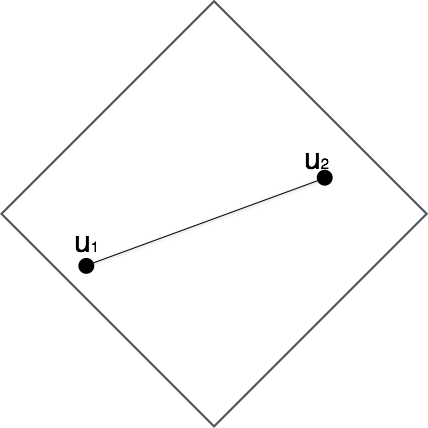
\includegraphics[width=\textwidth]{img/unit_l1_norm.png}
                \caption{$l1$ unit sphere.}
            \end{subfigure}
            \begin{subfigure}[b]{0.3\textwidth}
                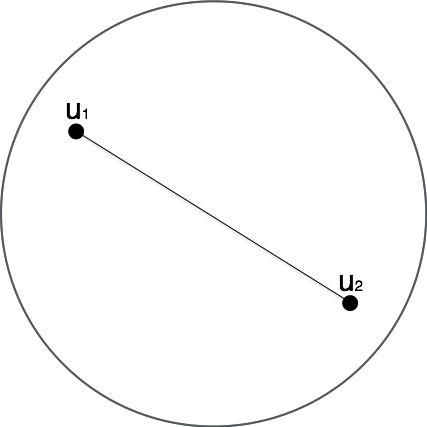
\includegraphics[width=\textwidth]{img/unit_l2_norm.png}
                \caption{$l2$ unit sphere.}
            \end{subfigure}
            \begin{subfigure}[b]{0.3\textwidth}
                
\includegraphics[width=\textwidth]{img/non_convex_set.png}
                \caption{Star: a non-convex set.}
            \end{subfigure}
            \caption[Examples of convex sets.]{Three different sets, where (a) and (b) are convex and (c) is non-convex. (a) is the unit sphere of the $l1$ norm, where (b) is the unit sphere of the $l2$ norm. In (c) we see that the line segment of $[u_{2}, u_{3}]$ does not fully lie in the set.}
            \label{fig:convex_and_non_convex_sets}
        \end{figure}
        \begin{definition}[Indicator Function, Support Function] % (fold)
        \label{def:indicator_function}
            For any convex subset $C$ of a vector space $X$, the indicator function $\delta_{C}: X \longrightarrow \mathbb{R}_{\infty}$ is defined as
                $$
                    \delta_{C}(u) =
                    \left\{
                        \begin{array}{l l}
                          0      & \quad \text{if $u \in C$} \\
                          \infty & \quad \text{if $u \notin C$}
                        \end{array}
                    \right. .
                $$
            The support function of the set $C$ is defined as
                $$
                    S_{C}(u) = \sup_{p \in C} \langle p, u \rangle,
                $$
            where we allow $S_{C}(u)$ to be $+\infty$.
    
        \end{definition}
        % definition indicator_function (end)
        \begin{definition}[Convex Function, Proper, Lower-Semicontinuous] % (fold)
        \label{def:convex_function_proper_lower_semicontinuous}
            Let $C \subseteq \mathbb{R}^{n}$ be a convex set. A function $F: C \longrightarrow [-\infty, \infty]$ is said to be
                \begin{itemize}
                    \item convex if and only if for all $u_{1}, u_{2} \in C$ and any $t \in [0, 1]$ the inequality
                    \begin{equation}
                        F(u_{1}t + u_{2}(1 - t)) \le F(u_{1})t + F(u_{2})(1 - t)
                        \label{eq:convex_function}
                    \end{equation}
                    is satisfied. $F$ is called strictly convex if Inequality (\ref{eq:convex_function}) holds strictly whenever $u_{1}, u_{2}$ are distinct points and $t \in (0, 1)$.
                    \item proper if and only if $F$ is not identically $-\infty$ or $+\infty$.
                    \item lower-semicontinuous (l.s.c) if and only if for any $u \in C$ and a sequence $(u_{n})$ converging to $u$,
                        $$
                            F(u) \le \liminf_{n \rightarrow \infty} F(u_{n}).
                        $$
                \end{itemize}
            We define $\Gamma_{0}(C)$ as the set of all convex, proper, l.s.c. functions on $C$.
        \end{definition}
        % definition convex_function_proper_lower_semicontinuous (end)
        A common example for a strictly convex function would be a quadratic function, cf. Example \ref{ex:convex_function} and Figure \ref{fig:convex_function} (a). It is illustrated together with the plot in (b) of the function
            \begin{equation}
                F(u) =
                    \begin{dcases*}
                        u^{2} & \textnormal{$x \in [-1, 1]$} \\
                        - \frac{1}{2} u(u - 4) & \textnormal{$x \in (1, 3]$}
                    \end{dcases*},
                \label{eq:lsc_example}
            \end{equation}
        which is a lower-semicontinuous function. The following theorem can for instance be found in \cite{Rockafellar}.
        \begin{theorem} % (fold)
            If $F, G$ are proper convex functions on $\mathbb{R}^{n}$, then $F + G$ is convex.
        \end{theorem}
        % theorem (end)
        \begin{proof} % (fold)
            Define $H(u) = F(u) + G(u)$ with $F, G$ being proper and convex and choose $u_{1}, u_{2} \in X$ and $t \in [0, 1]$. Then we obtain
            \begin{eqnarray}
                H(u_{1}t + u_{2}(1 - t)) &=& F(u_{1}t + u_{2}(1 - t)) + G(u_{1}t + u_{2}(1 - t)) \notag \\ 
                &\le& F(u_{1})t + F(u_{2})(1 - t) + G(u_{1})t + G(u_{2})(1 - t) \notag \\
                &=& \underbrace{F(u_{1})t + G(u_{1})t}_{= H(u_{1})t} + \underbrace{F(u_{2})(1 - t) + G(u_{2})(1 - t)}_{H(u_{2})(1 - t)} \notag \\
                &=& H(u_{1})t + H(u_{2})(1 - t). \notag
            \end{eqnarray}\qed
        \end{proof}
        % proof (end)
        \begin{remark}[Concave Function] % (fold)
            \label{rem:concave_function}
            If $-F$ is (strictly) convex, then we say that $F$ is (strictly) concave. If $F$ is both convex and concave we say that $F$ is affine, i.e. equality holds in Equation (\ref{eq:convex_function}).
        \end{remark}
        % remark concave_function (end)
        \begin{example} % (fold)
        \label{ex:convex_function}
            \begin{enumerate}
                \item Let $A \in \mathbb{R}^{n \times n}$ be a real, symmetric, positiv definite matrix and $F: \mathbb{R}^{n} \longrightarrow \mathbb{R}$ a linear function with $F(u) = \frac{1}{2}u^{T}Au + b^{T}u = \frac{1}{2}||u||_{A}^{2} + b^{T}u$, where $||\cdot||_{A}^{2}$ denotes the quadratic $A$-norm. Then $F$ is strictly convex. We can verify this with $t \in (0, 1)$ and
                    \begin{eqnarray}
                        F(u_{1}t + u_{2}(1-t)) &=& \frac{1}{2} ||u_{1}t + u_{2}(1-t)||_{A}^{2} + b^{T}(u_{1}t + u_{2}(1-t)) \notag \\
                        &\overbrace{\le}^{(\ast)}& \frac{1}{2} \left(||u_{1}t||_{A}^{2} + ||u_{2}(1-t)||_{A}^{2}\right) + (b^{T}u_{1})t + (b^{T}u_{2})(1-t) \notag \\
                        &=& \frac{1}{2} \left( \underbrace{t^{2}||u_{1}||_{A}^{2}}_{< t||u_{1}||_{A}^{2}} + \underbrace{(1-t)^{2}||u_{2}||_{A}^{2}}_{< (1-t)||u_{2}||_{A}^{2}} \right) + (b^{T}u_{1})t + (b^{T}u_{2})(1-t) \notag \\
                        &<& \underbrace{\frac{1}{2} t||u_{1}||_{A}^{2} + (b^{T}u_{1})t}_{= F(u_{1})t} + \underbrace{\frac{1}{2} (1-t)||u_{2}||_{A}^{2} + (b^{T}u_{2})(1-t)}_{= F(u_{2})(1-t)} \notag \\
                        &=& F(u_{1})t + F(u_{2})(1-t). \notag
                    \end{eqnarray}
                In $(\ast)$ we used the triangle inequality.
                \item Each norm $||\cdot||: X \longrightarrow \mathbb{R}$ on a normed vector space $X$ is convex (see also Figure \ref{def:convex_function_proper_lower_semicontinuous} for the $l1$ and $l2$ norm).
                    \begin{proof} % (fold)
                        Choose $u, v \in X, t \in [0, 1]$, then
                        $$
                            ||ut + v(1 - t)|| \overbrace{\le}^{(\ast)} ||ut|| + ||v(1 - t)|| \overbrace{=}^{(\ast\ast)} ||u|| t + ||v|| (1 - t).
                        $$
                        In $(\ast)$ we used the triangle inequality and in $(\ast\ast)$ absolute homogeneity with the fact that $t \in [0, 1]$ and for that $(1-t) \in [0,1]$.\qed
                    \end{proof}
                    % proof (end)
            \end{enumerate}
        \end{example}
        % example convex_function (end)
        There is another definition of convex functions. Therefore, let us first introduce the epigraph and the domain of a function.
        \begin{definition}[Domain, Epigraph] % (fold)
        \label{def:domain_epigraph}
            For any function $F: X \longrightarrow \mathbb{R}_{\infty}$, we define the domain
                $$
                    \textnormal{dom}(F) = \{ u \in X : F(u) < +\infty \}
                $$
            and the epigraph
                $$
                    \textnormal{epi}(F) = \{ (u, t) \in X \times \mathbb{R}: t \ge F(u) \} \in \mathbb{R}^{n+1}.
                $$
        \end{definition}
        % definition domain_epigraph (end)
        An illustration of the domain and epigraph can be seen in Figure \ref{fig:domain_epigraph}. In the previous definition we used that a function $F$ is convex if and only if its domain is convex. Now, we have an equivalent definition of convex functions by using the definition of the epigraph.
        \begin{definition}[Convex Function] % (fold)
        \label{def:convex_function_else}
            A function $F: X \longrightarrow \mathbb{R}$ is convex if and only if $\textnormal{epi}(F)$ is a convex set.
        \end{definition}
        \begin{figure}[!ht]
            \centering
            \begin{subfigure}[b]{0.4\textwidth}
            \begin{tikzpicture}[scale=0.8]
                \begin{axis}
                    \addplot[domain=-3:3,blue] {x*x};
                    \addplot[domain=-1:2,black] {x + 2};
                \end{axis}
            \end{tikzpicture}
            \caption{A quadratic function.}
            \end{subfigure}
            \begin{subfigure}[b]{0.4\textwidth}
            \begin{tikzpicture}[scale=0.8]
                \begin{axis}
                    \addplot[domain=-1:1,blue] {x*x};
                    \addplot[domain=1:3,blue] {-0.5*x*(x-4)};
                    \draw[dotted] (axis cs:1,-1) -- (axis cs:1,3);
                    \addplot[soldot] coordinates{(1,1)};
                    \addplot[holdot] coordinates{(1,1.5)};
                \end{axis}
            \end{tikzpicture}
            \caption{A l.s.c. function.}
            \end{subfigure}
            \caption[Example of a convex and a l.s.c. function.]{(a) The plot of one line segment above a quadratic function, which lies completely in $\textnormal{epi}(F)$. (b) The lower term $u^{2}$ accesses the value $(1,1)$, but the upper term of the function $-\frac{1}{2}u(u-4)$ does not.}
            \label{fig:convex_function}
        \end{figure}
        % definition convex_function_else (end)
        \begin{example}
            \label{ex:convex_function_reloaded}
            The indicator function $\delta_{C}: X \to \mathbb{R}_{\infty}$ of a set $C$ is convex if and only if $C$ is a convex set. This can be seen by:\\
            $"\Longrightarrow"$: If $\delta_{C}(u)$ is a convex function, we know that the domain of $\delta_{C}(u)$ is convex by Definition \ref{def:convex_function_else}. So, $C = \textnormal{dom}(\delta_{C}(u))$ is a convex set.\\
            $"\Longleftarrow"$: Reversely, if $C$ is a convex set the domain of $\delta_{C}(u)$ denoted by $\textnormal{dom}(\delta_{C}(u)) = C$ is convex. Then $\delta_{C}(u)$ is a convex function.
        \end{example}
        \begin{figure}[!ht]
            \centering
            \begin{tikzpicture}
                \begin{axis}
                    \addplot[domain=-1:1,black,fill=gray] {0.5*x*x};
                    \draw[red] (axis cs:-1,0) -- (axis cs:1,0);
                    \draw[red] (axis cs:-1,-0.02) -- (axis cs:-1,0.02);
                    \draw[red] (axis cs:1,-0.02) -- (axis cs:1,0.02);
                \end{axis}
            \end{tikzpicture}
            \caption[Domain and Epigraph.]{The domain (red) denoted as $\textnormal{dom}(F) = [-1, 1]$ and epigraph \\$\textnormal{epi}(F) = \{(u, t) \in [-1, 1] \times \mathbb{R} : t \ge \frac{1}{2}u^{2}\}$ (gray) of a function $F: [-1, 1] \longrightarrow \mathbb{R}$ with $F(u) = \frac{1}{2}u^{2}$.}
            \label{fig:domain_epigraph}
        \end{figure}
        Now that we are set up with convexity, we want to introduce an important concept which is used in this thesis.
        \begin{definition}[Legendre-Fenchel conjugate] % (fold)
        \label{def:legendre_fenchel_conjugate}
            Let $F: X \longrightarrow \mathbb{R}$. We define the Legendre-Fenchel conjugate $F^{\ast}$ of $F$ for any $p \in Y$ by
                \begin{equation}
                    F^{\ast}(p) = \sup_{u \in X} \left( \langle p, u \rangle - F(u) \right).
                    \label{eq:legendre_fenchel_conjugate}
                \end{equation}
        \end{definition}
        % definition legendre_fenchel_conjugate (end)
        \begin{remark} % (fold)
            \begin{itemize}
                \item Without a proof we state that $F^{\ast}$ - as the supremum of linear, continuous functions - is convex and lower-semicontinous, even $F$ is not convex. In addition, $F^{\ast}$ is proper if $F$ is convex and proper.
                \item In some literature the Legendre-Fenchel conjugate is also denoted as convex conjugate. We use these two expressions equivalently.
            \end{itemize}
        \end{remark}
        % remark (end)
        \begin{theorem} % (fold)
            Let $F \in \Gamma_{0}(X)$, then $F^{\ast\ast} = F$.
        \end{theorem}
        % theorem (end)
        The theorem assures that for a convex function $F$ we can rewrite Equation (\ref{eq:legendre_fenchel_conjugate}) into
            $$
                F(u) = \left( F^{\ast}(p) \right)^{\ast}(u) = \sup_{p \in Y} \left( \langle u, p \rangle - F^{\ast}(p) \right).
            $$
        A proof of this theorem can be found in \cite{Rockafellar}.
        \begin{example}
        \label{ex:legendre_fenchel_conjugate_example}
            Let us view some examples on the Legendre-Fenchel conjugate.
            \begin{enumerate}
                \item The Legendre-Fenchel conjugate of the indicator function of a set $C \subseteq X$ is given by
                    $$
                        \delta^{\ast}_{C}(p) = \sup_{u \in X} \left( \langle p, u \rangle - \delta_{C}(u) \right) = \sup_{u \in C} \langle p, u \rangle,
                    $$
                which is the support function of the set $C$.
                \item Let $F: X \to \mathbb{R}$ be a convex function and $\alpha > 0$. Then the convex conjugate of $\alpha F(u)$ is given by
                    $$
                        \alpha F^{\ast}(\frac{p}{\alpha}).
                    $$
                To verify this equality, we compute
                    $$
                        F^{\ast}(p) = \sup_{u \in X} \left( \langle p, u \rangle - \alpha F(u) \right) = \alpha \underbrace{\sup_{u \in X} \left( \langle \frac{p}{\alpha}, u \rangle - F(u) \right)}_{= F^{\ast}(\frac{p}{\alpha})} = \alpha F^{\ast}(\frac{p}{\alpha}).
                    $$
                \item Now, let $||\cdot||$ be a norm on $X$ with dual norm $||\cdot||_{\ast}$ on $Y$. We show that
                    $$
                        F^{\ast}(p) =
                            \begin{dcases*}
                                0 & \textnormal{if $||p||_{\ast} \le 1$} \\
                                \infty & \textnormal{else}
                            \end{dcases*}
                        = \delta_{||p||_{\ast} \le 1}(p),
                    $$
                i.e. the convex conjugate of a norm is the indicator function of the unit ball of its dual norm. We compute
                    $$
                        F^{\ast}(p) = \sup_{u \in X} \left( \langle p, u \rangle - ||u|| \right).
                    $$
                First assume that $||p||_{\ast} > 1$. By definition of the dual norm $||p||_{\ast} = \sup\limits_{||x|| \le 1} |\langle p, x \rangle|$ there is a $x \in \mathbb{R}^{n}$ for which we observe that $\langle p, x \rangle > 1$. We set $u = tx$ and let $t \longrightarrow \infty$, then we get
                    $$
                        \langle p, u \rangle - ||u|| = t(\langle p, x \rangle - ||x||) \longrightarrow \infty.
                    $$
                This shows $F^{\ast}(p) = \infty$. On the other hand if we assume that $||p||_{\ast} \le 1$, Cauchy-Schwarz-inequality assures
                    $$
                        \langle p, u \rangle \le ||u|| \, ||p||_{\ast}
                    $$
                for all $u \in X$. This implies
                    $$
                        \langle p, u \rangle - ||u|| \le ||u|| \, ||p||_{\ast} - ||u|| = ||u|| \, (||p||_{\ast} - 1) \le 0.
                    $$
                Since $||p||_{\ast} \le 1$ holds, we need to choose $u = 0$ to attain the supremum in $F^{\ast}(p)$. This shows that $F^{\ast} = \sup\limits_{u \in X} \left( \langle p, 0 \rangle - ||0|| \right) = 0$.
                \item As a last example we show that for a function $F(u) = \frac{1}{2} ||u||^{2}$ its convex conjugate is given by $F^{\ast}(p) = \frac{1}{2} ||p||_{\ast}^{2}$. With Cauchy-Schwarz-inequality we have
                    $$
                        \langle p, u \rangle - \frac{||u||^{2}}{2} \le ||p||_{\ast}\,||u|| - \frac{||u||^{2}}{2},
                    $$
                where the righthand side is a quadratic function of $||u||$. Define $H(x) := -\frac{x^{2}}{2} + y\,x$, then the maximal value of $H$ is $x = y$, since $H^{'}(x) = -x + y$ and $H^{''}(x) = -1 < 0$, then $H^{'}(x) = 0$ implies $x = y$. Setting $x = ||u||$ and $y = ||p||_{\ast}$ we have $||u|| = ||p||_{\ast}$. It follows
                    $$
                        \langle p, u \rangle - \frac{||u||^{2}}{2} \le ||p||_{\ast}||u|| - \frac{||u||^{2}}{2} = ||p||_{\ast} ||p||_{\ast} - \frac{||p||_{\ast}}{2} = \frac{||p||_{\ast}^{2}}{2}.
                    $$
                This shows that $F^{\ast}(p) = \sup\limits_{u \in X} \left( \langle u, p \rangle - \frac{||u||^{2}}{2} \right) \le \frac{||p||_{\ast}^{2}}{2}$. Let us now proof the inequality in the other direction. We assume that we find an arbitrary $u$ which satisfies $\langle u, p \rangle = ||u||\,||p||_{\ast}$. Further, we assume that $||u|| = ||p||_{\ast}$. Then we have
                    $$
                        \langle p, u \rangle - \frac{||u||^{2}}{2} = ||u||\,||p||_{\ast} - \frac{||u||^{2}}{2} = \frac{||p||^{2}_{\ast}}{2},
                    $$
                and conclude
                    $$
                        \frac{||p|_{\ast}^{2}}{2} = \langle p, u \rangle - \frac{||u||^{2}}{2} \le \sup\limits_{u \in X} \left( \langle p, u \rangle - \frac{||u||^{2}}{2} \right) = F^{\ast}(p).
                    $$
                From these two inequalities it follows that $F^{\ast}(p) = \frac{||p||_{\ast}^{2}}{2}$.
            \end{enumerate}
        \end{example}
        Another important property of functions is differentiability. Unfortunately, in some cases a function $F$ is not differentiable everywhere. As shown in Example \ref{ex:subgradient_subdifferential} the absolute value function is not differentiable in $0$. If a non-differentiable function is convex, we have a generalization of the derivative, called subderivative or subdifferential. For this, we want to define the subdifferential and corresponding to it, the subgradient.
        \begin{definition}[Subgradient, Subdifferential] % (fold)
        \label{def:subgradient_subdifferential}
            Let $X \subseteq \mathbb{R}^{n}$ be an open, convex set and $F: X \longrightarrow \mathbb{R}$ a convex function. A vector $y$ is called subgradient of $F$ in $u_{0} \in X$, if
                \begin{equation}
                    F(u) \ge F(u_{0}) + \langle y, u - u_{0} \rangle \,\,\, \forall u \in X.
                \label{eq:subgradient}
                \end{equation}
            The set
                $$
                    \partial F(u_{0}) = \{ y \in X: \, F(u) \ge F(u_{0}) + \langle y, u - u_{0} \rangle \,\,\, \forall u \in \textnormal{dom}(F) \}
                $$
            is called subdifferential of $F$ in $u_{0} \in X$ and $\textnormal{dom}(\partial F) = \{ u: \partial F(u) \ne \emptyset \} \subseteq F$.
        \end{definition}
        % definition subgradient_subdifferential (end)
        If $F$ and $G$ are differentiable, we have $\partial(F + G) = \partial F + \partial G$. For the subdifferential this holds under some conditions. We want to give the corresponding proposition without a proof, for which we refer to \cite{Rockafellar}. But, we state that in our computations this equality can always be used.
        \begin{proposition} % (fold)
            Let $F, G$ be convex and assume $\textnormal{int} (\textnormal{dom} G) \cap \textnormal{dom} F \ne \emptyset$: then
                $$
                    \partial(F + G) = \partial F + \partial G.
                $$
        \end{proposition}
        % proposition (end)
        To illustrate the subgradient and subdifferential, respectively, we want to give some examples.
        \begin{example}
        \label{ex:subgradient_subdifferential}
            \begin{enumerate}
                \item Take the absolute value function $F(u) = |u|$ in $\mathbb{R}$, defined by
                    $$
                        F(u) =
                            \begin{dcases*}
                                u & \textnormal{if $u \ge 0$,} \\
                                -u & \textnormal{else}.
                            \end{dcases*}
                    $$
                Since $F(u)$ is not differentiable in $0$, but on $\mathbb{R} \setminus \{0\}$, we compute the subgradient $y$ at a point $u_{0}$ by
                    \begin{itemize}
                        \item $\partial F(u_{0}) = 1$ if $u_{0} > 0$,
                        \item $\partial F(u_{0}) = -1$ if $u_{0} < 0$,
                        \item and finally if $u_{0} = 0$
                            $$
                                F(0) + y (u - 0) \le F(u) \iff y u \le |u|.
                            $$
                        If $u \ge 0$ this is equivalent to $y \le 1$. If $u < 0$ we get
                            $$
                                y u \le |u| \iff y u \le -u \iff y \ge -1.
                            $$
                    \end{itemize}
                We get the subgradient in $u_{0}$ with
                    $$
                        y =
                            \left\{
                                \begin{array}{l l}
                                    1 & \textnormal{if $u_{0} > 0$} \\
                                    -1 & \textnormal{if $u_{0} < 0$} \\
                                    $\textnormal{[-1, 1]}$ & \textnormal{if $u_{0} = 0$}
                                \end{array}
                            \right.
                    $$
                and in addition the subdifferential for all $u \in \textnormal{dom}(F(u))$
                    $$
                        \partial F(u) =
                            \left\{
                                \begin{array}{l l}
                                    1 & \textnormal{if $u > 0$} \\
                                    -1 & \textnormal{if $u < 0$} \\
                                    $\textnormal{[-1,1]}$ & \textnormal{if $u = 0$}
                                \end{array}
                            \right. .
                    $$
                \item Let $F(u) = ||u||_{1}$ be the $l1$ norm, which is defined by
                    $$
                        ||u||_{1} := \sum_{i = 1}^{n} |u_{i}|,
                    $$
                for $u \in \mathbb{R}^{n}$. As a non-differentiable function in $u_{0} = 0$, we seek for the subdifferential. Looking at the i-th component of the subgradient, we evaluate the subgradient of the absolute value function. With the first example, we know that $y_{i} = -1$ if $u_{0_{i}} < 0$ and $y_{i} = 1$ if $u_{0_{i}} > 0$. In the case, where $u_{0_{i}} = 0$, we have $y_{i} \in [-1,1]$. Overall, we set
                    $$
                        y_{i} =
                            \left\{
                                \begin{array}{l l}
                                    1 & \textnormal{if $u_{0_{i}} > 0$} \\
                                    -1 & \textnormal{if $u_{0_{i}} < 0$} \\
                                    $\textnormal{[-1, 1]}$ & \textnormal{if $u_{0_{i}} = 0$}
                                \end{array}
                            \right.
                    $$
                for all $i = 1, ..., n$. Note that for the whole vector $y$ the inequality $||y||_{\infty} \le 1$ is satisfied. Then, the subdifferential is given by
                    $$
                        \partial F(u) = \left\{ y : ||y||_{\infty} \le 1, \, \langle y, u \rangle = ||x||_{1} \right\}.
                    $$
            \end{enumerate}
        \end{example}
        The following proposition can be found in the work of Pock and Chambolle (\cite{Chambolle-et-al-10}). We provide it without a proof.
        \begin{proposition} % (fold)
        \label{prop:zero_element_of_subgradient}
            
            Let $F$ be convex, then $\hat{u} \in \arg \min\limits_{u \in X} F(u)$ if and only if $0 \in \partial F(\hat{u})$.

        \end{proposition}
        % proposition zero_element_of_subgradient (end)
        Another important property of convex minimization problems is summarized in the next proposition. It can be found in \cite{Rockafellar}, along with a proof.
        \begin{proposition} % (fold)
        \label{prop:global_minimum}

            Let $F \in \Gamma_{0}(X)$. Then if $\hat{u}$ is a local minimum of $F$, then $\hat{u}$ is in fact a global minimum, i.e.
                    $$
                        \hat{u} \in \arg \min_{u \in X} F(u).
                    $$
        \end{proposition}
        % proposition (end)
        These two propositions give us some important statements. If we find a (local) minimizer of a convex minimization problem, we already know that this minimizer is indeed the global minimal value. Further, we can verify that a solution of a minimization problem is valid, if zero is an element of the subdifferential of the cost function at this specific minimal point. With this, we later compute the proximity operator of the functions in our underlying models. This operator is defined in the next definition and is also used in Moreau's theorem (cf. Theorem \ref{the:moreau_identity}).
        \begin{definition}[Projection Operator, Proximity Operator, Moreau Envelop] % (fold)
        \label{def:projection_operator}

            For any non-empty closed set $C$ the projection operator for an arbitrary point $z \notin C$ onto the set $C$ is defined by
                \begin{equation}
                    \Pi_{C}(z) = \arg \min_{u \in C} \frac{1}{2} ||z - u||_{2}^{2},
                \end{equation}
            meaning the orthogonal projection onto $C$. We define the proximity operator in a similar fashion due to
                \begin{equation}
                    \textnormal{prox}^{\alpha}_{F}(z) = \arg \min_{u \in X} \frac{1}{2} ||u - z||_{2}^{2} + \alpha \, F(u),
                    \label{eq:proximity_operator}
                \end{equation}
            and the Moreau envelop as
                $$
                    M^{\alpha}_{F}(z) = \min_{u \in X} \frac{1}{2} ||u - z||_{2}^{2} + \alpha \, F(u),
                $$
            for any $\alpha > 0$.
        \end{definition}
        % definition projection_operator (end)
        The next theorem, namely Moreau's theorem, was first proven in 1965 by Jean J. Moreau and can be found in \cite{Rockafellar}, along with a proof.
        \begin{theorem}[Moreau's Theorem] % (fold)
        \label{the:moreau_identity}

            Let $F$ be a closed proper convex function on $\mathbb{R}^{n}$ and $F^{\ast}(p)$ its convex conjugate. Then
                $$
                    M^{1}_{F}(z) + M^{1}_{F^{\ast}}(z) = \frac{1}{2}||z||_{2}^{2},
                $$
            i.e. for each $z \in \mathbb{R}^{n}$ one has
                $$
                    \min_{u \in X} \left( \frac{1}{2} ||u - z||_{2}^{2} + F(u) \right) + \min_{p \in Y} \left( \frac{1}{2} ||p - z||_{2}^{2} + F^{\ast}(p) \right) = \frac{1}{2}||z||_{2}^{2},
                $$
            where both minima are uniquely attained. The unique vectors $u$ and $p$ for which the respective minima are attained for a given $z$ are the unique vectors $u$ and $p$ such that
                \begin{equation}
                    z = u + p, \,\,\,\,\, p \in \partial F(u),
                    \label{eq:equivalence_of_moreau_property}
                \end{equation}
            and they are given by
                \begin{equation}
                    u = \textnormal{prox}^{1}_{F}(z), \,\,\,\,\, p = \textnormal{prox}^{1}_{F^{\ast}}(z).
                    \label{eq:prox_z}
                \end{equation}
        \end{theorem}
        % theorem moreau_identity (end)
        \begin{remark}
            Another way to denote the proximity operator is the notation
                \begin{equation}
                    \textnormal{prox}^{\alpha}_{F}(z) = (\textnormal{Id} + \alpha \partial F)^{-1}(z).
                    \label{eq:proximity_operator_reloaded}
                \end{equation}
            It can be derived by Proposition \ref{prop:zero_element_of_subgradient}. So, we assume that $\hat{u} \in \textnormal{prox}^{\alpha}_{F}$. Then
                $$
                    0 \in \partial \left( \alpha F(\hat{u}) + \frac{1}{2} ||\hat{u} - z||_{2}^{2} \right) = \alpha \, \partial F(\hat{u}) + \hat{u} - z.
                $$
            But this can be rewritten to
                $$
                    z \in \alpha\,\partial F(\hat{u}) + \hat{u} \iff \hat{u} = (\textnormal{Id} + \alpha \, \partial F)^{-1}(z).
                $$
            According to Chambolle et al. in \cite{Chambolle-et-al-10}, we get due to Moreau the following identity:
                \begin{equation}
                    z = (\textnormal{Id} + \alpha \, \partial F)^{-1}(z) + \alpha \left( \textnormal{Id} + \frac{1}{\alpha} \partial F^{\ast} \right)^{-1} \left(\frac{z}{\alpha}\right).
                    \label{eq:moreau_identity_reloaded}
                \end{equation}
            This equation is best known as Moreau's identity. For $\alpha = 1$ we observe
                $$
                    z = (\textnormal{Id} + \partial F)^{-1}(z) + \left( \textnormal{Id} + \partial F^{\ast} \right)^{-1} (z).
                $$
        \end{remark}
        To this end, let us discuss some examples on the projection and proximity operator, respectively.
        \begin{example}
        \label{ex:projection_operator}
            \begin{itemize}
                \item The $lp$ projection of a point $\tilde{u} \in \mathbb{R}^{n}$ onto the $l^{p}$ unit sphere with $\tilde{u} \notin C = \{u : ||u||_{p} \le 1 \}$ is given by the following minimization problem:
                    \begin{equation}
                        \begin{array}{l l}
                            \min\limits_{u \in \mathbb{R}^{n}} &  \frac{1}{2} ||u - \tilde{u}||_{2}^{2} \\
                            \textnormal{subject to} & ||u||_{p} \le 1.
                        \end{array}
                        \notag
                    \end{equation}
                According to \cite{Jitkomut} the $l2$ and the $l^{\infty}$ projection are given by
                    \begin{enumerate}
                        \item $\Pi_{||\cdot||_{2} \le 1}(\tilde{u}) = \frac{\tilde{u}}{\max(1, |\tilde{u}|)}$, or equivalently
                            \begin{equation}
                                u^{\ast} =
                                \left\{
                                    \begin{array}{l l}
                                       \tilde{u} & \textnormal{if}\,\, ||\tilde{u}||_{2} \le 1 \\
                                       \frac{\tilde{u}}{||\tilde{u}||_{2}} & \textnormal{otherwise}
                                    \end{array}
                                \right.
                                \notag
                            \end{equation}
                        \item and $\Pi_{||\cdot||_{\infty} \le 1}(\tilde{u}) = \min(1, \max(-1, \tilde{u}))$, or for all $k = 1, ..., n$
                            \begin{equation}
                                u_{k}^{\ast} =
                                \left\{
                                    \begin{array}{l l}
                                       \tilde{u}_{k} & \textnormal{if}\,\, |\tilde{u}_{k}| \le 1 \\
                                       1 & \textnormal{otherwise}
                                    \end{array}
                                \right. .
                                \notag
                            \end{equation}
                    \end{enumerate}
                \item If we set $F(u) = \delta_{C}(u)$ then we compute the proximity operator by
                $$
                    \textnormal{prox}^{\alpha}_{F}(\tilde{u}) = \min\limits_{u \in X} \frac{||u - \tilde{u}||_{2}^{2}}{2} + \alpha \, \delta_{C}(u) = \min\limits_{u \in C} \frac{||u - \tilde{u}||_{2}^{2}}{2} = \Pi_{C}(\tilde{u}).
                $$
                We see a connection between the two operators. Proximation of the indicator function is the same as doing a euclidean projection onto the corresponding set $C$.
            \end{itemize}
        \end{example}
    % section convex_optimization_and_convex_analysis (end)
    \section{Total Variation} % (fold)
    \label{sec:total_variation}
        
        The definition of the total variation, the variation of functions and functions of bounded variation can be found in \cite{Giusti}, together with the first example in this section. The total variation is the basis when talking about variational methods in image processing. We cover this topic superficial, but this is enough in our context.
        \begin{definition}[Total Variation] % (fold)
        \label{def:total_variation}
            Let $\Omega$ be an open subset of $\mathbb{R}^{n}$. For a function $u \in L^{1}(\Omega)$, the \textnormal{total variation} of $u$ in $\Omega$ is defined as
                $$
                    \textnormal{TV}(u) = \sup \bigg\{ -\int_{\Omega} u\, \textnormal{div}\, (\varphi)\, dx : \varphi \in C^{1}_{0}(\Omega, \mathbb{R}^{n}), |\varphi(x)| \le 1, \forall x \in \Omega \bigg\}.
                $$
        \end{definition}
        % definition total_variation (end)
        \begin{example} % (fold)
        \label{prop:u_is_smooth}
            Let $u \in W_{1}^{1}(\Omega)$, then integration by parts and $\varphi$ having compact support leads to
                \begin{eqnarray}
                    -\langle u, \textnormal{div}\,(\varphi) \rangle &=& - \int_{\Omega} u\, \textnormal{div}\, (\varphi)\, dx \notag \\
                    &=& - \left( \underbrace{\int_{\partial\Omega} u\, \varphi\, d\mathcal{H}^{n-1}}_{= 0} - \int_{\Omega} \nabla\,u\, \varphi\, dx \right) = \int_{\Omega} \nabla\,u\,\varphi\,dx \notag \\
                    &=& \langle \nabla u, \varphi \rangle,
                    \label{eq:nabla_equals_minus_divergence}
                \end{eqnarray}
            for every $\varphi \in C^{1}_{0}(\Omega, \mathbb{R}^{n})$ so that
                \begin{equation}
                    \textnormal{TV}(u) = \int_{\Omega} |\nabla\,f| dx.
                    \label{eq:tvl1}
                \end{equation}
            The idea to derive Equation (\ref{eq:tvl1}) is that we first evaluate the case where
                $$
                    \textnormal{TV}(u) \le \int_{\Omega} |\nabla\,f| dx.
                $$
            This can be seen by using Cauchy-Schwarz-inequality
                \begin{eqnarray}
                    \int_{\Omega} \nabla u \, \varphi \, dx &\le& \bigg| \int_{\Omega} \nabla u \, \varphi dx \bigg| \, dx \notag \\
                    &\le& \int_{\Omega} |\nabla u| \, \underbrace{|\varphi|}_{\le 1} \, dx \le \int_{\Omega} |\nabla u| \, dx. \notag
                \end{eqnarray}
            For the inequality in the other direction, the key idea would be to set $\varphi = \frac{\nabla u}{|\nabla u|}$. Then, $|\varphi| = 1$. Since $\varphi \notin C_{0}^{1}$ we would approximate $\varphi$ in $L1$. This space lies close in the space of smooth functions with compact support and for that satisfies the assumptions.
        \end{example}
        % example u_is_smooth (end)
        \begin{remark}
            Note that $W_{1}^{1}(\Omega)$ denotes the $L1$-Sobolev-Space of $\Omega$, which means that $u \in L^{1}(\Omega)$ and $Du \in L^{1}(\Omega)$. Here, $Du$ is meant in the sense of distributional derivatives. Further note that the total variation is convex and lower-semicontinous. See \cite{Chambolle-et-al-10} for details.
        \end{remark}
        To get a better intuition of the total variation, we want to propose the defintion of the variation of functions $u \in [a, b] \subseteq \mathbb{R}$.
        \begin{definition}[Variation of a function] % (fold)
        \label{def:variation_of_a_function}
            Let $u: \mathbb{R} \longrightarrow \mathbb{R}$ and $a < b$ be real numbers. Then define the variation of $u$ on $[a, b]$ as
                $$
                    V^{b}_{a}(u) = \sup \bigg\{ \sum_{i = 1}^{n} |u(x_{i}) - u(x_{i - 1})| : n \in \mathbb{N} \,\textnormal{and}\, a = x_{0} < x_{1} < ... < x_{n} = b \bigg\}.
                $$
        \end{definition}
        % definition variation_of_a_function (end)
        This definition is well known and suited for functions from $\mathbb{R}$ to $\mathbb{R}$. According to \cite{Giusti} this definition is ill-posed in the sense of measures and integrals.
        \begin{example} % (fold)
        \label{ex:total_variation_one_d}
            Let $a, b \in \mathbb{R}$ with $a < b$. If $u: [a, b] \longrightarrow \mathbb{R}$ is monotonically increasing, then for any $a = x_{0} < x_{1} < ... < x_{n} = b$ we observe
                \begin{eqnarray}
                    &&\sum_{i = 1}^{n} |u(x_{i}) - u(x_{i-1})| = \sum_{i = 1}^{n} u(x_{i}) - u(x_{i-1}) \notag \\
                    &=& u(x_{1}) - u(x_{0}) + u(x_{2}) - u(x_{1}) + ... + u(x_{n-1}) - u(x_{n-2}) + u(x_{n}) - u(x_{n-1}) \notag \\
                    &=& u(x_{n}) - u(x_{0}) = u(b) - u(a). \notag
                \end{eqnarray}
            It follows that $V^{b}_{a}(u) = \sup \{u(b) - u(a)\} = u(b) - u(a)$.
        \end{example}
        % example total_variation_one_d (end)
        Another class of functions, which is considered in Chapter \ref{cha:minimizing_the_mumford_shah_functional}
        are (special) functions of bounded variation. Even though we do not explicitly make use of this class of functions, we want to give the definitions for the sake of completeness. Further, (special) functions of bounded variation are strongly related to total variation as the following definition ensures (see for instance \cite{Giusti}).
        \begin{definition}[Functions of bounded variation]
        \label{def:functions_of_bounded_variation}
            A function $u \in L^{1}(\Omega)$ is said to have bounded variation in $\Omega$ if $\textnormal{TV}(u) < \infty$. We define $BV(\Omega)$ as the space of all functions in $L^{1}(\Omega)$ with bounded variation. This space is equipped with the norm
                $$
                    ||u||_{BV} = ||u||_{L^{1}} + \int_{\Omega} |Du|,
                $$
            and for that it is a Banach space.
        \end{definition}
        % definition functions_of_bounded_variation (end)
        Relating to Example \ref{ex:total_variation_one_d} we find that $u \in BV(\mathbb{R})$, since $V^{b}_{a}(u) = u(b) - u(a) < \infty$ for $a, b \in \mathbb{R}$, $a < b$.
        Additionally, $BV$-functions are proper and we have if $u \in BV(\Omega)$ then also $u \in \Gamma_{0}(\Omega)$, because the total varition is convex and l.s.c. (see again \cite{Chambolle-et-al-10}).
        \begin{definition}[Special functions of bounded variation \cite{Pock-et-al-iccv09}]
            $SBV$ denotes the special functions of bounded variation, i.e. functions $u$ of bounded variation for which the derivative $Du$ is the sum of an absolutely continuous part $\nabla u \cdot dx$ and a discontinuous singular part $S_{u}$.
        \end{definition}
        This class of functions plays a role, when applying convex relaxation techniques to the Mumford-Shah functional. But, as mentioned, the definition is only given for the sake of completeness in this thesis and we will not explicitly make use of it.

    % section total_variation (end)

% chapter basic_concepts (end)

\chapter{The ROF, TVL1 and Mumford-Shah Functional} % (fold)
\label{cha:the_rof_tvl1_and_mumford_shah_functional}

    In this chapter we consider convex optimization problems, namely minimization of the ROF and TVL1 functional. Furthermore, we seek for a minimizer of the non-convex Mumford-Shah functional. We apply techniques of convex analysis to turn these minimization into saddle-point problems. In the case of the Mumford-Shah functional we also use these techniques, even if the functional itself is non-convex. There is no proof that this strategy yields the minimal value of the Mumford-Shah functional. Nonetheless, this approach leads to high-quality image approximations.

    Our goal is to approximate an input image $g$ by a function $u$. The underlying functionals are modeled with two terms and we try to minimize the energy of each functional, to find a good approximation. We consider problems of the form
        $$
            minimize \,\,\, \left( \textnormal{Functional} \right) = minimize \,\,\, \left( \textnormal{Data Fidelity Term} + \textnormal{Regularizer Term} \right).
        $$
    The data fidelity term assures that an approximation $u$ is as close to the input image $g$ as possible. The regularizer adds further assumptions to the model, for example seeks for smoothness of the approximation $u$ in specific regions. Before we consider the three models of this chapter, we need some definitions and notations.

    \section{The General Saddle-Point Problem} % (fold)
    \label{sec:the_general_saddle_point_problem}
        
        Let us begin by introducing the general class of problems we consider. For this, we follow Chambolle et al. (\cite{Chambolle-et-al-10} Section 3.5 and \cite{Chambolle10afirst-order} Chapter 2). We define the map $K: X \longrightarrow Y$ as a continuous linear operator with induced norm
            $$
                ||K|| = \max \left\{ ||Kx||_{Y} : x \in X \,\, \textnormal{with} \,\, ||x||_{X} \le 1 \right\}.
            $$
        Furthermore, we define the map $K^{\ast}: Y \longrightarrow X$ as the adjoint operator of $K$.\\
        Let $u \in X$, $p \in Y$ and define $G: X \longrightarrow [0, +\infty)$ and $F^{\ast}: Y \longrightarrow [0, +\infty)$ where $G, F^{\ast} \in \Gamma_{0}$ and $F^{\ast}$ being the Legendre-Fenchel conjugate of a convex, l.s.c. function $F$. We are trying to find a saddle point $(u, p)$ of the following problem:
            \begin{equation}
                \min_{u \in X} \max_{p \in Y} \left( \langle Ku, p \rangle + G(u) - F^{\ast}(p) \right).
                \label{eq:the_saddle_point_problem}
            \end{equation}
        We also call this saddle-point problem the primal-dual problem, where $u$ is the primal and $p$ the dual variable. We define the corresponding primal problem by
            \begin{equation}
                \min_{u \in X} \left( G(u) + F(Ku) \right)
                \label{eq:primal_problem}
            \end{equation}
        and the dual problem by
            \begin{equation}
                \max_{p \in Y} -(G^{\ast}(-K^{\ast}p) + F^{\ast}(p)).
                \label{eq:dual_problem}
            \end{equation}
        We can show that these three different classes of problems are equivalent if $F$ itself is convex. Then, the convex conjugate assures that $F(Ku) = \sup_{p \in Y} \left( \langle p, Ku \rangle - F^{\ast}(p) \right)$. Further, the so called \textit{Von Neumann's minimax theorem} must hold, cf. \cite{Zeidler}. It states that the objective function needs to be convex in the primal and concave in the dual variable and the feasible set for $u$ or the feasible set for $p$ must be compact. With this we get
            \begin{eqnarray}
                \min_{u \in X} \left(F(Ku) + G(u)\right) &=& \min_{u \in X} \max_{p \in Y} \left(\langle p, Ku \rangle - F^{\ast}(p) + G(u) \right) \notag \\
                &=& \max_{p \in Y} \min_{u \in X} \left(\langle K^{\ast}p, u \rangle + G(u) - F^{\ast}(p) \right) \notag \\
                &=& \max_{p \in Y} \left( -\max_{u \in X} -\left( \langle K^{\ast}p, u \rangle + G(u) \right) - F^{\ast}(p) \right) \notag \\
                &=& \max_{p \in Y} \left( \underbrace{-\max_{u \in X} \left( \langle -K^{\ast}p, u \rangle - G(u) \right)}_{= -G^{\ast}(-K^{\ast}p)} - F^{\ast}(p) \right) \notag \\
                &=& \max_{p \in Y} -(G^{\ast}(-K^{\ast}p) + F^{\ast}(p)). \notag
            \end{eqnarray}
        Note, that we will provide the dual probles of the ROF and TVL1 model. In these two particular cases all conditions are satisfied. Finding the optimal value $\hat{u}$ for the primal problem can for instance be done by a gradient descent in $u$. On the other hand, if $\hat{p}$ is an optimal value, we can find it by a gradient ascent in $p$ of the dual problem. The basic idea of the primal-dual algorithm, presented in the next section, is then to do both, a gradient descent in $u$ and a gradient ascent in $p$, simultaneously, to solve the saddle-point problem.
    % section the_general_saddle_point_problem (end)

    \section{A Primal-Dual Algorithm} % (fold)
    \label{sec:a_firs_order_primal_dual_algorithm}

        According to Chambolle et al. in \cite{Chambolle-et-al-10}, the idea of the primal-dual algorithm goes back to Arrow and Hurwicz, see \cite{Arrow-Hurwicz}, and the first time this algorithm was stated in such a framework was probably in \cite{Appleton-Talbot}. As mentioned in the last section, we simultaneously compute a gradient descent in $u$ and a gradient ascent in $p$. After each ascent and descent, respectively, we apply the proximity operator for $F^{\ast}$ and $G$, respectively, to the estimated values. Choosing time-steps $\sigma, \tau > 0$ we get
            $$
                \left\{ 
                    \begin{array}{l l}
                        p^{n+1} = (\textnormal{Id} + \sigma\,\partial\,F^{\ast})^{-1}(p^{n} + \sigma\,Ku^{n})\\
                        u^{n+1} = (\textnormal{Id} + \tau\,\partial\,G)^{-1}(u^{n} - \tau\,K^{\ast}p^{n+1})
                  \end{array}
                \right. .
            $$
        The scheme was first proposed in a paper of Zhu and Chan in \cite{Zhu-Chan}. Unfortunately, there is no proof of convergence for it. But in 2009 Pock, Cremers, Bischof and Chambolle published a paper (\cite{Pock-et-al-iccv09}) that we also consider in Chapter \ref{cha:minimizing_the_mumford_shah_functional}, whose contribution was an extension of the above scheme for which convergence can be guaranteed under certain conditions. The idea is to attach an additional extrapolation step to the algorithm, as seen in line three of the Primal-Dual Algorithm \ref{alg:primal_dual_algorithm}. In \cite{Chambolle10afirst-order}, Pock and Chambolle generalized this algorithm. They also proposed some variations of the algorithm itself. Depending on the properties of the corresponding functions $F^{\ast}$ and $G$ one can derive, for instance, a better convergence rate. We will not show details of this and only make use of the first algorithm proposed in \cite{Chambolle10afirst-order}. Additionally, we consider a variant of this algorithm, proposed in \cite{Strekalovskiy-Cremers-eccv14}. Furthermore, we will not provide a proof of convergence for these algorithms. For details, we refer again to \cite{Chambolle10afirst-order}. The general primal-dual algorithm can be written as follows:
        \begin{algorithm}[Primal-Dual Algorithm]
        \label{alg:primal_dual_algorithm}
            Choose $(u^{0}, p^{0}) \in X \times Y$ and let $\bar{u}^{0} = u^{0}$. Further let $\tau, \sigma > 0$ and $\theta \in [0, 1]$. Then, we let for each $n \ge 0$
                $$
                    \left\{ 
                        \begin{array}{l l}
                            p^{n+1} = (\textnormal{Id} + \sigma\,\partial\,F^{\ast})^{-1}(p^{n} + \sigma\,K\bar{u}^{n}) \\
                            u^{n+1} = (\textnormal{Id} + \tau\,\partial\,G)^{-1}(u^{n} - \tau\,K^{\ast}p^{n+1}) \\
                            \bar{u}^{n+1} = u^{n+1} + \theta (u^{n+1} - u^{n})
                        \end{array}
                    \right. .
                $$
        \end{algorithm}
        Computing $p^{n} + \sigma\,K\bar{u}^{n}$ and $u^{n} - \tau\,K^{\ast}p^{n+1}$ is easy, since these two are sums of vectors. The last line of this scheme is again the summation of vectors. In the next section, we introduce the notation for $K$ and $K^{\ast}$. We will see that computing the linear operators applied to $u$ and $p$ is quite simple. Computing the proximity operators in line one and two of the algorithm needs further work and varies within each model. We will compute the proximity operators for each model explicitly in the corresponding sections. If all updates for $u, p$ and $\bar{u}$ are computed, this iteration scheme solves saddle-point problems of the form (\ref{eq:the_saddle_point_problem}).
        \begin{remark}
            In the theorem of convergence, found in \cite{Chambolle10afirst-order}, we have that convergence is guaranteed if we set the chosen parameters $\tau$ and $\sigma$ appropriately. Additionally, the algorithm is independent of initialization. As long as the inequality $\tau\sigma L^{2} < 1$ is satisfied, where $L = ||K||$ is the bound on the norm of the linear operator $K$, convergence is guaranteed. The better the choice for these parameters beforehand, the faster the algorithm converges. Estimating the best time-steps is ongoing research. A first approach was a preconditioning scheme, published in \cite{Pock2011} by Pock and Chambolle. Of course, it is not the best way having an algorithm which is dependent on manually chosen parameters. But, on the other hand, the parameter $\tau$ is controllable, with respect to the fact that $\sigma$ can be computed from $\tau$ by $\sigma = \frac{1}{\tau * L^{2}}$. Despite the fact that we then have $\tau\sigma L^{2} = 1$, convergence is still given, according to the first remark in \cite{Chambolle10afirst-order}.

            Note that in our computations we always set $\theta = 1$. So, the third line of the algorithm becomes
                $$
                    \bar{u}^{n+1} = 2u^{n+1} - u^{n}.
                $$
        \end{remark}
        The convergence rate for our primal-dual algorithm is $\mathcal{O}\left(\frac{1}{N}\right)$. A variant of this proposed algorithm can be found in the work of Strekalovskiy and Cremers (\cite{Strekalovskiy-Cremers-eccv14}) and will be used for the real-time minimization framework of the Mumford-Shah functional.
        \begin{algorithm}[Real-Time Primal-Dual Algorithm]
        \label{alg:realtime_primal_dual_algorithm}
            Choose $(u^{0}, p^{0}) \in X \times Y$ and let $\bar{u}^{0} = u^{0} = f$. Further let $\tau_{0} = \frac{1}{2d}, \sigma_{0} = \frac{1}{2}$. Then, we let for each $n \ge 0$ as long as $||u^{n+1} - u^{n}|| < \varepsilon$
                $$
                    \left\{ 
                        \begin{array}{l l}
                            p^{n+1} = (\textnormal{Id} + \sigma_{n}\,\partial\,F^{\ast})^{-1}(p^{n} + \sigma_{n}\,K\bar{u}^{n}) \\
                            u^{n+1} = (\textnormal{Id} + \tau_{n}\,\partial\,G)^{-1}(u^{n} - \tau_{n}\,K^{\ast}p^{n+1}) \\
                            \theta_{n} = \frac{1}{\sqrt{1 + 4\tau_{n}}}, \, \tau_{n+1} = \theta_{n}\tau_{n}, \, \sigma_{n+1} = \frac{\sigma_{n}}{\theta_{n}} \\
                            \bar{u}^{n+1} = u^{n+1} + \theta_{n} (u^{n+1} - u^{n})
                        \end{array}
                    \right. .
                $$
        \end{algorithm}
        The difference of this scheme to Algorithm \ref{alg:primal_dual_algorithm} is that $\tau$ and $\sigma$ are determined by initialization. Further, they are updated, together with $\theta$, in each iteration step. These updates lead to a better convergence rate, namely $\mathcal{O}\left(\frac{1}{N^{2}}\right)$. But, this approach is only applicable if $G$ or $F^{\ast}$ is uniformly convex (see also \cite{Chambolle10afirst-order}, Algorithm 2).

    % section a_firs_order_primal_dual_algorithm (end)

    \section{Discrete Setting} % (fold)
    \label{sec:discrete_setting}

        On computers images are discrete objects, with discrete pixel locations. For that, we need a proper notation for our framework. In our discrete setting we consider a regular pixel grid of size $N \times M$ and set
            \begin{equation}
                \mathcal{G} = \bigg\{ (i, j) : i = 1, ..., N \,\, \textnormal{and} \,\, j = 1, ..., M \bigg\},
                \label{eq:pixel_grid}
            \end{equation}
        where the indices $(i, j)$ denote the discrete locations in the pixel grid. We define an image $u \in X: \mathcal{G} \longrightarrow \mathbb{R}$ where $X \in \mathbb{R}^{N \times M}$ is a finite dimensional vector space equipped with the standard inner product
            \begin{equation}
                \langle u, v \rangle_{X} = u^{T}v = \sum_{i = 1}^{N} \sum_{j = 1}^{M} u_{i, j} v_{i, j}, \,\,\, u, v \in X
                \label{eq:inner_product}
            \end{equation}
        and the standard euclidean norm
            $$
                ||u||_{2} = \langle u, u \rangle^{\frac{1}{2}}, \,\,\, u \in X.
            $$
        Furthermore, let $Y = X \times X$ be the dual space of $X$, equipped with the inner product defined by
            \begin{equation}
                \langle p, q \rangle_{Y} = p^{T}q = \sum_{i = 1}^{N} \sum_{j = 1}^{M} p^{1}_{i, j} q^{1}_{i, j} + p^{2}_{i, j} q^{2}_{i, j},
                \label{eq:inner_product_space_y}
            \end{equation}
        with $p_{i, j} = \left(p^{1}_{i, j}, p^{2}_{i, j}\right)^{T}, q_{i, j} = \left(q^{1}_{i, j}, q^{2}_{i, j}\right)^{T} \in Y$, also equipped with the euclidean norm. Additionally, we define two important norms. The discrete isotropic total variation norm is given by
            $$
                ||\nabla \, u||_{1} = \sum_{i = 1}^{N} \sum_{j = 1}^{M} |(\nabla \, u)_{i, j}|, \,\,\, \textnormal{where} \,\,\, |(\nabla \, u)_{i, j}| = \sqrt{((\nabla \, u)^{1}_{i, j})^{2} + ((\nabla \, u)^{2}_{i, j})^{2}}
            $$
        and the discrete maximum norm by
            $$
                ||p||_{\infty} = \max_{i, j} |p_{i, j}|, \,\,\, \textnormal{where} \,\,\, |p_{i, j}| = \sqrt{(p^{1}_{i, j})^{2} + (p^{2}_{i, j})^{2}}.
            $$
        It is left to present the representation of the linear operator $K$. Relating to the definition of the total variation in Equation (\ref{eq:nabla_equals_minus_divergence}) we have $\langle \nabla u, p \rangle = - \langle u, \textnormal{div}\,(p) \rangle$. In a finite dimensional vector space we have $\langle \nabla u, p \rangle = \langle u, \nabla^{T} p \rangle$ if $\nabla$ is a matrix. For this, we set $K = \nabla$ and $K^{\ast} = \nabla^{T} = -\textnormal{div}$.
        \begin{definition}[Discrete gradient operator] % (fold)
        \label{def:discrete_gradient_operator}
            We define the discrete gradient of a vector $u \in X$ by $\nabla u = ((\partial_{i}u)_{i, j}, (\partial_{j}u)_{i, j})^{T}$ using forward differences with Neumann boundary conditions, i.e.
                \begin{eqnarray}
                    (\partial_{i}u)_{i, j} =
                        \begin{dcases*}
                            u_{i+1, j} - u_{i, j} & \textnormal{if $i < N$}\\
                            0 & \textnormal{if $i = N$}
                        \end{dcases*}, \notag \\
                    (\partial_{j}u)_{i, j} =
                        \begin{dcases*}
                            u_{i, j+1} - u_{i, j} & \textnormal{if $j < M$}\\
                            0 & \textnormal{if $j = M$}
                        \end{dcases*}. \notag
                \end{eqnarray}
        \end{definition}
        % definition discrete_gradient_operator (end)
        \begin{definition}[Discrete divergence operator] % (fold)
        \label{def:discrete_divergence_operator}
            We define the discrete divergence of a vector $p \in Y$ by $\nabla^{T} p = (\partial_{i}p^{1})_{i, j} + (\partial_{j}p^{2})_{i, j}$ using backward differences with Dirichlet boundary conditions, i.e.
                \begin{eqnarray}
                    (\partial_{i}p^{1})_{i, j} =
                        \begin{dcases*}
                            p^{1}_{i, j} - p^{1}_{i-1, j} & \textnormal{if $1 < i < N$}\\
                            p^{1}_{i, j} & \textnormal{if $i = 1$}\\
                            -p^{1}_{i-1, j} & \textnormal{if $i = N$}
                        \end{dcases*}, \notag \\
                    (\partial_{j}p^{2})_{i, j} =
                        \begin{dcases*}
                            p^{2}_{i, j} - p^{2}_{i, j-1} & \textnormal{if $1 < j < M$}\\
                            p^{2}_{i, j} & \textnormal{if $j = 1$}\\
                            -p^{2}_{i, j-1} & \textnormal{if $j = M$}
                        \end{dcases*}. \notag
                \end{eqnarray}
        \end{definition}
        % definition discrete_gradient_operator (end)
        We show that these two definitions resemble $K = \nabla$ and $K^{\ast} = \nabla^{T} = -\textnormal{div}$. For that, we first take a look at the matrices $(\nabla)^{1}$ and $(\nabla)^{2}$ of the gradient operator in Definition \ref{def:discrete_gradient_operator}. We have
            $$
                (\nabla)^{1} = 
                \begin{pmatrix}
                    -1 & & & & \\
                    1 & -1 & & & \\
                      & \ddots & \ddots & & \\
                      & & 1 & -1 & \\
                      & & & 1 & 0
                \end{pmatrix} \,\,\, \textnormal{and} \,\,\,
                (\nabla)^{2} =
                \begin{pmatrix}
                    -1 & 1 & & & \\
                      & -1 & 1 & & \\
                      & & \ddots & \ddots & \\
                      & & & -1 & 1 \\
                      & & & & 0
                \end{pmatrix},
            $$
        as the two components of $\nabla$. On the other hand, if we analyse the two components of $\nabla^{T}$, we observe
            $$
                (\nabla^{T})^{1} = 
                \begin{pmatrix}
                    1 & -1 & & & \\
                      & 1 & -1 & & \\
                      & & \ddots & \ddots & \\
                      & & & 1 & -1 \\
                      & & & & 0
                \end{pmatrix} \,\,\, \textnormal{and} \,\,\,
                (\nabla^{T})^{2} =
                \begin{pmatrix}
                    1 & & & & \\
                    -1 & 1 & & & \\
                      & \ddots & \ddots & & \\
                      & & -1 & 1 & \\
                      & & & -1 & 0
                \end{pmatrix}.
            $$
        With this representation, we see that 
            $$
                -((\nabla)^{1})^{T} = -(\textnormal{div})^{1} = (\nabla^{T})^{1} \,\,\,\,\, \textnormal{and} \,\,\,\,\, -((\nabla)^{2})^{T} = -(\textnormal{div})^{2} = (\nabla^{T})^{2}.
            $$
        We additionally compute the bound on the norm of these two operators, where we follow the notation of Pock and Chambolle in \cite{Chambolle10afirst-order}.
        \begin{proposition}[Bound on the norm of $\nabla$] % (fold)
            \label{prop:bound_on_the_norm}

            The bound on the norm of the proposed discrete linear operators is given by
                $$
                    L^{2} = ||K|| = ||\nabla||^{2} = ||\nabla^{T}||^{2} \le 8.
                $$
        \end{proposition}
        % proposition bound_on_the_norm (end)
        \begin{proof} % (fold)
            We set $p^{1}_{0,j} = 0$ and $p^{2}_{i,0} = 0$. Then we compute
                \begin{eqnarray}
                    L^{2} &=& ||\nabla||^{2} = ||\nabla^{T}||^{2} = \max_{||p||_{Y} \le 1} ||\nabla^{T}\,p||^{2}_{X} \notag \\
                    &=& \max_{||p||_{Y} \le 1} \sum_{i = 1}^{N} \sum_{j = 1}^{M} \left( p^{1}_{i, j} - p^{1}_{i-1, j} + p^{2}_{i, j} - p^{2}_{i, j-1} \right)^{2} \notag \\
                    &\overbrace{\le}^{(\ast)}& 4 \max_{||p||_{Y} \le 1} \sum_{i = 1}^{N} \sum_{j = 1}^{M} (p^{1}_{i, j})^{2} + (p^{1}_{i-1, j})^{2} + (p^{2}_{i, j})^{2} + (p^{2}_{i, j-1})^{2} \notag \\
                    &\le& 8 \max_{||p||_{Y} \le 1} ||p||^{2}_{Y} = 8, \notag
                \end{eqnarray}
            in $(\ast)$ we used Young's inequality $ab \le \frac{a^{p}}{p} + \frac{b^{q}}{q}$ twice, with $p = q = 2$.\qed
        \end{proof}
        % proof (end)
    % section discrete_setting (end)

    \section{The ROF Model} % (fold)
    \label{sec:the_rof_model}
        
        Now, that everything is defined properly we consider the minimization of the ROF functional, named after Leonid I. Rudin, Stanley Osher and Emad Fatemi. This functional was first proposed in 1992 in \cite{ROF}. It is the prototype when talking about variational methods in image processing.
        \begin{definition}[ROF Functional] % (fold)
        \label{def:the_rof_functional}
            Let $\Omega \in \mathbb{R}^{n}$ be the $n$-dimensional image domain, $u \in W_{1}^{1}(\Omega)$ and $g \in L^{1}(\Omega)$ an input image. Then the ROF functional is defined as
                \begin{equation}
                    E_{ROF}(u) = \textnormal{TV}(u) + \frac{\lambda}{2} \int_{\Omega} |u - g|^{2} \, dx = \int_{\Omega} |\nabla \, u| \, dx + \frac{\lambda}{2} \int_{\Omega} |u - g|^{2} \, dx
                    \label{eq:the_rof_model}
                \end{equation}
            and we seek to compute the minimizer over all $u$.
        \end{definition}
        % definition the_rof_model (end)
        The appearing parameter $\lambda$ is used to handle the tradeoff between the regularizer, the total variation, and the data fidelity term which is a least squares term. Using a larger value for $\lambda$ we get an approximation $u$ which is closer to the input image $g$. If we choose $\lambda$ to be small the weighting of the regularizer is higher. For that, the approximation $u$ is smoother, because the gradient in the total variation penalizes jumps in the approximation $u$. Reformulation of Equation (\ref{eq:the_rof_model}) into a discrete minimization problem gives us:
            \begin{equation}
                \min_{u \in X} E_{ROF}(u) = \min_{u \in X} ||\nabla \, u||_{1} + \frac{\lambda}{2} ||u - g||_{2}^{2},
            \label{eq:discrete_rof_model}
            \end{equation}
        with $u \in X$ being the unknown approximation and $g \in X$ the given data. This minimization problem is convex because the cost function as a sum of norms is convex. Let us now rewrite the model, the minimization of the ROF functional, into a saddle-point formulation.

        \subsection{ROF Model as Saddle-Point Problem} % (fold)
        \label{sub:rof_model_as_saddle_point_problem}

            In order to obtain a saddle-point formulation of Equation (\ref{eq:discrete_rof_model}), we identify the functions $F(\nabla u) = ||\nabla \, u||_{1}$ and $G(u) = \frac{\lambda}{2} ||u - g||_{2}^{2}$, respectively. Hence, we face
                \begin{equation}
                    \min_{u \in X}\,\, F(\nabla u) + G(u) = \min_{u \in X}\,\, ||\nabla \, u||_{1} + \frac{\lambda}{2} ||u - g||_{2}^{2}.
                \label{eq:primal_rof_problem}
                \end{equation}
            Since $F$ is a convex function, we can express it in terms of its convex conjugate by
                $$
                    F(\nabla u) = F^{\ast\ast}(\nabla u) = \sup\limits_{p \in Y} \left(\langle p, \nabla \, u \rangle - F^{\ast}(p) \right).
                $$
            We observe, by inserting the expression of $F(\nabla u)$ into Equation (\ref{eq:primal_rof_problem}), the saddle-point problem
                $$
                    \min_{u \in X}\, \max_{p \in Y}\,\, \langle p, \nabla \, u \rangle - F^{\ast}(p) + G(u).
                $$
            It remains to show how $F^{\ast}(p)$ is represented. From Example \ref{ex:legendre_fenchel_conjugate_example} 2. and the fact that the conjugate norm of the $l1$ norm is the $l^{\infty}$ norm, we have
                $$
                    F^{\ast}(p) =
                        \begin{dcases*}
                            0 & \textnormal{if $||p||_{\infty} \le 1$} \\
                            \infty & \textnormal{else}
                        \end{dcases*},
                $$
            or equivalently $F^{\ast}(p) = \delta_{P}(p)$ for a set $P$ given by
                \begin{equation}
                    P = \left\{ p \in Y : ||p||_{\infty} \le 1 \right\}.
                    \label{eq:the_set_P}
                \end{equation}
            Using this information, we seek to solve the saddle-point problem
                \begin{equation}
                    \min_{u \in X}\, \max_{p \in Y}\,\, \langle p, \nabla\, u \rangle + \frac{\lambda}{2} ||u - g||_{2}^{2} - \delta_{P}(p).
                \label{eq:primal_dual_rof_problem}
                \end{equation}
            We also want to propose the dual formluation of Equation (\ref{eq:primal_dual_rof_problem}). For that, we need to compute $G^{\ast}$. Set $v = u - g$ which is equivalent to $u = v + g$ and compute
                \begin{eqnarray}
                    G^{\ast}(p) &=& \sup_{u \in X} \left( \langle u, p \rangle - \frac{\lambda}{2} ||u - g||_{2}^{2} \right) \notag \\
                    &=& \sup_{v \in X} \left( \langle v + g, p \rangle - \frac{\lambda}{2} ||v||_{2}^{2} \right) \notag \\
                    &=& \underbrace{\left( \sup_{v \in X} \langle v, p \rangle - \frac{\lambda}{2} ||v||_{2}^{2} \right)}_{= \frac{1}{2\lambda} ||p||_{2}^{2} \,\,\, (\ast)} + \langle g, p \rangle \notag \\
                    &=& \frac{1}{2\lambda} ||p||_{2}^{2} + \langle g, p \rangle. \notag
                \end{eqnarray}
            In $(\ast)$ we used Examples \ref{ex:legendre_fenchel_conjugate_example} 2. and 4. Inserting $F^{\ast}$ and $G^{\ast}$, respectively, into Equation (\ref{eq:dual_problem}) and setting $K^{\ast} = \nabla^{T} = -\textnormal{div}$ we get the dual formulation by
                \begin{eqnarray}
                    \max_{p \in Y}\,\, -(G^{\ast}(-K^{\ast}p) + F^{\ast}(p)) &=& \max_{p \in Y} - \left( \frac{1}{2\lambda} ||-\nabla^{T}p||^{2}_{2} + \langle g, -\nabla^{T}p \rangle_{X} + \delta_{P}(p) \right) \notag \\
                    &=& \max_{p \in Y} - \left( \frac{1}{2\lambda} ||\textnormal{div}\,(p)||^{2}_{2} + \langle g, \textnormal{div}\,(p) \rangle_{X} + \delta_{P}(p). \right) \notag
                \end{eqnarray}
            Let us now compute the corresponding proximity operators of Problem (\ref{eq:primal_dual_rof_problem}), to be able to solve this saddle-point problem using the primal-dual algorithm.
            % subsection rof_model_as_saddle_point_problem (end)
        \subsection{The Proximity Operators of the ROF Model} % (fold)
        \label{sub:the_proximity_operators_for_the_rof_model}

            In Algorithm \ref{alg:primal_dual_algorithm} we presented how saddle-point problems can be solved efficiently. In two of the three steps of the proposed primal-dual algorithm we needed the proximity operators
                $$
                    (\textnormal{Id} + \sigma\,\partial\,F^{\ast})^{-1} \,\,\, \textnormal{and} \,\,\, (\textnormal{Id} + \tau\,\partial\,G)^{-1}.
                $$
            Within the saddle-point problem in (\ref{eq:primal_dual_rof_problem}) we identify $G(u) = \frac{\lambda}{2} ||u - g||_{2}^{2}$ and therefore $F^{\ast}(p) = \delta_{P}(p)$. With the identity of Equation (\ref{eq:proximity_operator}) we compute the proximity operator of the indicator function $\delta_{P}(p)$ by
                $$
                    (\textnormal{Id} + \sigma\,\partial\,F^{\ast})^{-1}(\tilde{p}) = \arg \min_{p \in Y} \frac{||p - \tilde{p}||_{2}^{2}}{2} + \sigma\,\delta_{P}(p) = \arg \min_{p \in P} \frac{||p - \tilde{p}||_{2}^{2}}{2}.
                $$
            This is nothing but the euclidean projection of a vector $\tilde{p} \notin P$ onto the convex set $P$. As we follow Pock and Chambolle in \cite{Chambolle10afirst-order}, we note that $P$ is the cross product of pointwise $L2$ balls, see also Figure \ref{fig:pointwise_l2_projections}. So, we compute pointwise euclidean (l2) projections. We get with Example \ref{ex:projection_operator} 1.
                $$
                    p = (\textnormal{Id} + \sigma\,\partial\,F^{\ast})^{-1}(\tilde{p}) = \Pi_{P}(\tilde{p}) \iff p_{i,j} = \frac{\tilde{p}_{i, j}}{\max(1, |\tilde{p}_{i, j}|)},
                $$
            for all $i = 1, ..., N, j = 1, ..., M$.
            \begin{figure}[!ht]
                \centering
                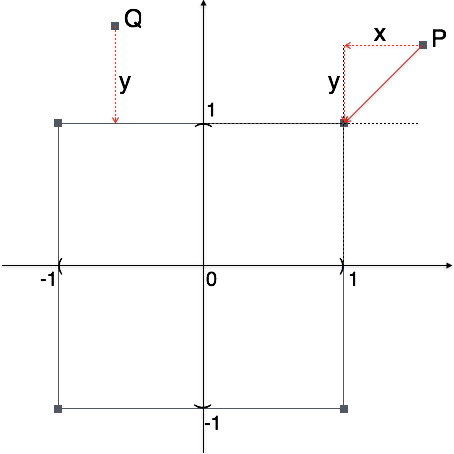
\includegraphics[width=0.5\textwidth]{img/pointwise_projection.png}
                \caption[Pointwise $l2$ projections.]{The point $P \in \mathbb{R}^{2}$ needs two pointwise projections. First in the direction of $x$ and afterwards in $y$ direction. The point $Q \in \mathbb{R}^{2}$ only needs one pointwise projection in the direction of $y$.}
                \label{fig:pointwise_l2_projections}
            \end{figure}

            It remains to compute the proximity operator for the function $G$. Here, we have
                $$
                    (\textnormal{Id} + \tau\,\partial\,G)^{-1}(\tilde{u}) = \arg \min_{u \in X} \frac{||u - \tilde{u}||_{2}^{2}}{2} + \frac{\tau\lambda}{2} ||u - g||_{2}^{2} = \arg \min_{u \in X} \mathcal{L}(u).
                $$
            Since $\mathcal{L}(u)$, as a sum of quadratic norms, is convex, a local minimizer is also a global minimizer. Let $\hat{u} \in \arg \min\limits_{u \in X} \mathcal{L}(u)$. With Proposition \ref{prop:zero_element_of_subgradient} we observe
                $$
                    0 \in \partial \mathcal{L}(\hat{u}) \iff 0 \in (\hat{u} - \tilde{u}) + \tau\lambda (\hat{u} - g) \iff (1 + \tau\lambda)\hat{u} = \tilde{u} + \tau\lambda g
                $$
            and this implies $\hat{u} = \frac{\tilde{u} + \tau\lambda g}{1 + \tau\lambda}$. Overall, the equivalence
                \begin{equation}
                    u = (\textnormal{Id} + \tau\,\partial\,G)^{-1}(\tilde{u}) \iff u_{i,j} = \frac{\tilde{u}_{i,j} + \tau\lambda g}{1 + \tau\sigma}
                \label{eq:proximity_operator_g_rof}
                \end{equation}
            holds pointwise for all $i = 1, ..., N$ and $j = 1, ..., M$. As a last step we show an appropriate stopping criterion to determine convergence of the primal-dual algorithm.
        % subsection the_proximity_operators_for_the_rof_model (end)

        \subsection{Stopping Criterion} % (fold)
        \label{sub:stopping_criterion_rof}

            We have several possibilities to determine convergence. As we seek to find the minimal energy of the ROF functional we could stop the algorithm as soon as this energy does not change too much. Hence, we compute
                $$
                    |E_{ROF}(u^{n+1}) - E_{ROF}(u^{n})| \le \varepsilon,
                $$
             for a $\varepsilon$ small enough. Estimating the whole energy once every iteration step in the primal-dual algorithm would generate computational overhead and for that slow down the code. We partially follow the idea proposed in \cite{Strekalovskiy-Cremers-eccv14} by Strekalovskiy and Cremers, but use another threshold for $\varepsilon$ and evaluate once every iteration
                $$
                    ||u^{n+1} - u^{n}|| \le \varepsilon,
                $$
            with $\varepsilon = \cdot 10^{-6}$. Furthermore, the underlying norm is defined by
                $$
                    ||\tilde{u}|| = \frac{1}{N \cdot M} \sum_{k = 1}^{B} \sum_{i = 1}^{N} \sum_{j = 1}^{M} |\tilde{u}_{i,j}|.
                $$
            Here, $B$ is the number of color channels. We set $B = 1$ for grayscaled and $B = 3$ for colored images, like RGB valued images. This computation is not as costly as the calculation of the whole energy function and as Chapter \ref{cha:applications_to_imaging} shows, a good criterion to determine convergence.

        % subsection stopping_criterion_rof (end)

    % section the_rof_model (end)

    \section{The TVL1 Model} % (fold)
    \label{sec:the_tvl1_model}
        
        The idea of the TVL1 functional is to replace the squared $L2$ norm in the data fidelity term $G(u) = ||u - g||_{2}^{2}$ with the $L1$ norm. This norm is more robust in removing the so called salt and pepper noise, meaning noisy extrem values white or black in an input image $g$. The name of this functional rises from the fact that it also uses the total variation as a regularization term. The functional is defined as follows:
        \begin{definition}[TVL1 Functional] % (fold)
        \label{def:tvl1_functional}

            Let $\Omega \in \mathbb{R}^{n}$ be the $n$-dimensional image domain, $u \in W_{1}^{1}(\Omega)$ and $g \in L^{1}(\Omega)$ an input image. Then the TVL1 functional is defined as
                \begin{equation}
                    E_{TVL1}(u) = \textnormal{TV}(u) + \lambda \int_{\Omega} |u - g| \, dx = \int_{\Omega} |\nabla \, u| \, dx + \lambda \int_{\Omega} |u - g| \, dx
                \end{equation}
            and we seek to compute the minimizer of this functional over all $u$.

        \end{definition}
        % definition the_tvl1_model (end)
        The parameter $\lambda$ handles the tradeoff between the data fidelity and the regularizer term, as seen in the ROF model. In this functional $\lambda$ controls the total variation term. This means a higher value on $\lambda$ amounts more smoothness in the approximation $u$. A lower value assures that $u$ is closer to the input image $g$. The discrete primal formulation is represented by
            \begin{equation}
                \min_{u \in X} E_{TVL1}(u) = \min_{u \in X} ||\nabla \, u||_{1} + \lambda ||u - g||_{1}.
                \label{eq:primal_formulation_tvl1}
            \end{equation}
        As done before, we want to turn this minimization problem into a saddle-point problem. Then, we are able to apply the primal-dual algorithm and for that solve this optimization problem.

        \subsection{TVL1 as Saddle-Point Problem} % (fold)
        \label{sub:tvl1_as_saddle_point_problem}

            Let us first note that the function $F(\nabla u)$, namely the total variation, remains the same as in the ROF model. Expressing $F$ in terms of its convex, as in Subsection \ref{sub:rof_model_as_saddle_point_problem}, we obtain
                $$
                    \min_{u \in X}\, \max_{p \in Y}\,\, \langle p, \nabla \, u \rangle - F^{\ast}(p) + G(u).
                $$
            Adapting $F^{\ast} = \delta_{P}(p)$ and the set $P$ as in Equation (\ref{eq:the_set_P}), we observe the primal-dual formulation
                $$
                    \min_{u \in X}\, \max_{p \in Y}\,\, \langle p, \nabla\, u \rangle + \lambda ||u - g||_{1} - \delta_{P}(p).
                $$
            For the representation of the dual problem of the TVL1 saddle-point problem we need to compute $G^{\ast}$. We find that the convex conjugate of the function  $G(u) = \lambda||u-g||_{1}$ is given by
                $$
                    G^{\ast}(p) =
                        \begin{dcases*}
                            \langle p, g \rangle & \textnormal{if $||p||_{\infty} \le \lambda$} \\
                            \infty & \textnormal{else}
                        \end{dcases*},
                $$
            or equivalently $G^{\ast}(p) = \delta_{Q}(p) + \langle p, g \rangle$ for a set
                $$
                    Q = \left\{ p \in Y : ||p||_{\infty} \le \lambda \right\}.
                $$
            To derive this representation of the conjugate function we set $z = u - g$ which is equivalent to $u = z + g$. Then with the definition of the convex conjugate we get
                \begin{eqnarray}
                    G^{\ast}(p) = \sup_{u \in X} \left( \langle p, u \rangle - G(u) \right) \iff G^{\ast}(p) &=& \sup_{z \in X} \left( \langle p, z + g \rangle - G(z + g) \right) \notag \\
                    &=& \sup_{z \in X} \left( \langle p, z + g \rangle - \lambda ||z||_{1} \right) \notag \\
                    &=& \sup_{z \in X} \left( \langle \frac{1}{\lambda} p, z \rangle - ||z||_{1} \right) + \langle p, g \rangle. \notag
                \end{eqnarray}
            Using Example \ref{ex:legendre_fenchel_conjugate_example} 2. and the fact that the conjugate norm of the $l1$ norm is the $l^{\infty}$ norm, leads us to
                $$
                    G^{\ast}(p) =
                        \begin{dcases*}
                            \langle p, g \rangle & \textnormal{if $||\frac{1}{\lambda}p||_{\infty} \le 1$} \\
                            \infty & \textnormal{else}
                        \end{dcases*} \iff
                    G^{\ast}(p) =
                        \begin{dcases*}
                            \langle p, g \rangle & \textnormal{if $||p||_{\infty} \le \lambda$} \\
                            \infty & \textnormal{else}
                        \end{dcases*}.
                $$
            Or equivalently $G^{\ast}(p) = \delta_{Q}(p) + \langle p, g \rangle$. The dual formulation of the TVL1 saddle-point problem is then given by
                \begin{eqnarray}
                    \max_{p \in Y}\,\, -(G^{\ast}(-K^{\ast}p) + F^{\ast}(p)) &=& \max_{p \in Y} -\left( \delta_{Q}(-\nabla^{T}\,p) + \langle -\nabla^{T}p, g \rangle + \delta_{P}(p) \right) \notag \\
                    &=& \max_{p \in Y} -\left( \delta_{Q}(\textnormal{div}\,(p)) + \langle \textnormal{div}\,(p), g \rangle + \delta_{P}(p) \right). \notag
                \end{eqnarray}
            It remains to compute the proximity operators for the functions $G$ and $F^{\ast}$.
        
        % subsection tvl1_as_saddle_point_problem (end)

        \subsubsection{The Proximity Operators of the TVL1 Model} % (fold)
        \label{ssub:the_proximity_operators_of_the_tvl1_model}
            
            The proximity operator of $F^{\ast}$ remains the same as in Subsection \ref{sub:the_proximity_operators_for_the_rof_model}. We have
                $$
                    p = (\textnormal{Id} + \sigma\,\partial\,F^{\ast})^{-1}(\tilde{p}) \iff p_{i,j} = \frac{\tilde{p}_{i, j}}{\max(1, |\tilde{p}_{i, j}|)},
                $$
            for all $i = 1, ..., N, j = 1, ..., M$. To compute the proximity operator of the function $G$ we get
                $$
                    (\textnormal{Id} + \tau\,\partial\,G)^{-1}(\tilde{u}) = \arg \min_{u \in X} \frac{||u - \tilde{u}||_{2}^{2}}{2} + \lambda\tau||u - g||_{1}.
                $$
            Therefore, we define $\mathcal{L}(u) = \frac{||u - \tilde{u}||_{2}^{2}}{2} + \lambda\tau||u - g||_{1}$, which is - as the sum of convex terms - a convex function. Let $\hat{u} \in \arg \min\limits_{u \in X} \mathcal{L}(u)$. Then with Proposition \ref{prop:zero_element_of_subgradient} we have that
                $$
                    0 \in \partial \mathcal{L}(\hat{u}) \iff 0 \in \hat{u} - \tilde{u} + \tau\lambda \partial(||\hat{u} - g||_{1}).
                $$
            By evaluating the $(i,j)$-th component of $\partial\mathcal{L}(\hat{u})$ we have
                \begin{eqnarray}
                    0 \in \partial_{i,j} \mathcal{L}(\hat{u}) &\iff& 0 \in \hat{u}_{i,j} - \tilde{u}_{i,j} + \tau\lambda \partial_{i,j}(||\hat{u} - g||_{1}) \notag \\
                    &\iff& 0 \in \hat{u}_{i,j} - \tilde{u}_{i,j} + \tau\lambda \partial_{i,j} (|\hat{u}_{i,j} - g_{i,j}|). \notag
                \end{eqnarray}
            This means we need to compute the subgradient of the absolute value function for all partial subderivatives $(i,j)$ with $i = 1, ..., N$, $j = 1, ..., M$. In Example \ref{ex:subgradient_subdifferential} 1. we saw how the subgradient for the absolute-value function is computed. We have
                $$
                    y_{i,j} =
                        \left\{
                            \begin{array}{l l}
                                1 & \textnormal{if $\hat{u}_{i,j} - g_{i,j} > 0$} \\
                                -1 & \textnormal{if $\hat{u}_{i,j} - g_{i,j} < 0$} \\
                                $\textnormal{[-1, 1]}$ & \textnormal{if $\hat{u}_{i,j} - g_{i,j} = 0$}
                            \end{array}
                        \right. ,
                $$
            where $y_{i,j}$ is the subgradient of the $(i,j)$-th component of $|\hat{u}_{i,j} - g_{i,j}|$. We check all three cases:
                \begin{enumerate}
                    \item Let $y_{i,j} = 1$. Then we obtain
                        $$
                            0 \in \hat{u}_{i,j} - \tilde{u}_{i,j} + \tau\lambda \iff \hat{u}_{i,j} = \tilde{u}_{i,j} - \tau\lambda.
                        $$
                    With $\hat{u}_{i,j} - g_{i,j} > 0$ and $\hat{u}_{i,j} = \tilde{u}_{i,j} - \tau\lambda$ this equation holds if 
                        $$
                            \tilde{u}_{i,j} - \tau\lambda - g_{i,j} > 0 \iff \tilde{u}_{i,j} - g_{i,j} > \tau\lambda.
                        $$
                    \item Now, let $y_{i,j} = -1$. We get
                        $$
                            0 \in \hat{u}_{i,j} - \tilde{u}_{i,j} - \tau\lambda \iff \hat{u}_{i,j} = \tilde{u}_{i,j} + \tau\lambda.
                        $$
                    Using this equality in the constraint, where $y_{i,j} = -1$, leads us to
                        $$
                            \tilde{u}_{i,j} + \tau\lambda - g_{i,j} > 0 \iff \tilde{u} - g_{i,j} > \tau\lambda.
                        $$
                    \item Finally, let $y_{i,j} \in [-1, 1]$ with $\hat{u}_{i,j} = g_{i,j}$. We get
                        $$
                            0 \in g_{i,j} - \tilde{u}_{i,j} + \tau\lambda y_{i,j} \iff \tilde{u}_{i,j} - g_{i,j} = \tau\lambda y_{i,j}.
                        $$
                    We apply the absolute value function to each side of the last equation and note that $|y_{i,j}| \le 1$. Then
                        $$
                            |\tilde{u}_{i,j} - g_{i,j}| = |\tau\lambda y_{i,j}| \le \tau\lambda.
                        $$
                \end{enumerate}
            Overall, we set for all $i = 1, ..., N$, $j = 1, ..., M$
                \begin{equation}
                    u = (\textnormal{Id} + \tau\,\partial\,G)^{-1}(\tilde{u}) \iff u_{i, j} = 
                        \begin{dcases*}
                            \tilde{u}_{i,j} - \tau\lambda & \textnormal{if\, $\tilde{u}_{i,j} - g_{i,j} > \tau\lambda$} \\
                            \tilde{u}_{i,j} + \tau\lambda & \textnormal{if\, $\tilde{u}_{i,j} - g_{i,j} < - \tau\lambda$} \\
                            g_{i, j} & \textnormal{if\, $|\tilde{u}_{i,j} - g_{i,j}| \le \tau\lambda$}
                        \end{dcases*}.
                \label{eq:prox_g_tvl1}
                \end{equation}
            As we computed all operators, which are necessary for the primal-dual algorithm, we need an appropriate criterion for convergence. We completely adapt the idea of Subsection \ref{sub:stopping_criterion_rof}. As shown in Chapter \ref{cha:applications_to_imaging}, it is also a well-suited criterion to determine convergence for minimizing the TVL1 functional.
        % subsubsection the_proximity_operators_of_the_tvl1_model (end)
    % section the_tvl1_model (end)

    \section{The Mumford-Shah Model} % (fold)
    \label{sec:the_mumford_shah_model}
        
        In the previous sections we showed that we can rewrite convex minimization into saddle-point problems. Further, we computed the proximity operators for the underlying functions in these models. With these, we were able to apply the primal-dual algorithm to solve each saddle-point problem. In this section we introduce a non-convex functional, namely the Mumford-Shah functional, we seek to minimize. The idea is, despite the non-convexity, to apply convex analysis to the minimization problem and use Moreau's identity to compute one of the proximity operators. Let us start by defining the Mumford-Shah functional.
        \begin{definition}[The Mumford-Shah Functional] % (fold)
        \label{def:the_mumford_shah_functional}
            Let $\Omega \subseteq \mathbb{R}^{2}$ be a rectangular image domain. In order to approximate an input image $g: \Omega \longrightarrow \mathbb{R}^{k}$ in terms of a piecewise smooth function $u: \Omega \longrightarrow \mathbb{R}^{k}$, the Mumford-Shah Functional is given by
                    
                    \begin{equation}
                        E_{MS}(u) = \int_{\Omega} (u - g)^{2} dx + \lambda \int_{\Omega \setminus K} |\nabla u|^{2} dx + \nu |K|,
                    \end{equation}
                    \label{eq:the_mumford_shah_functional}
                
                where $\nu, \lambda > 0$ are weighting parameters and $k$ is the number of color channels. Further, $K = K_{1} \cup ... \cup K_{N}$ and $|K|$ denotes the length of the curves $K$.
        \end{definition}
        % definition the_mumford_shah_functional (end)
        \begin{remark}
            In this section we follow the representation of the Mumford-Shah functional of \cite{Strekalovskiy-Cremers-eccv14}.
        \end{remark}
        This functional differs from the ones in the previous sections. The first term, the data fidelity term, remains the same as in the ROF model, except a scaling factor $\frac{1}{2}$ and the parameter $\lambda$ now controls the first term of the regularizer. This regularizer consists of two terms in this functional. The first term of the Mumford-Shah regularizer uses again the gradient, but not in the set $\Omega$ itself. Instead it states that the approximation $u$ should be smooth in sets of $\Omega$ separated by curves $K$, namely in $\Omega \setminus K$. We call $K$ the discontinuity set (or jump set). The length of the discontinuity set $K$ is also measured and taken into account in the energy $E_{MS}(u)$. We find two weighting parameters $\nu$ and $\lambda$ in this model. Where $\lambda$ handles the tradeoff between the first term of the regularizer and the data fidelity term, $\nu$ controls the length of the discontinuity set $K$. A smaller $\nu$ yields a smoother image, where a higher $\nu$ leads to sharper edges in the approximation. Yet, the parameter $\lambda$ plays another important role. If we choose $\lambda$ small enough then the model is also called piecewise-smooth Mumford-Shah model. On the other hand, in the limiting case $\lambda \to \infty$, we can only attain a minimum if we set $\nabla u = 0$ in $\Omega \setminus K$. Then the model is known as the piecewise-constant Mumford-Shah model. In \cite{Strekalovskiy-Cremers-eccv14} Strekalovskiy and Cremers suggested to rewrite the regularizer in the discrete setting by using the following function:
            \begin{equation}
                R_{MS}(f) = \min(\lambda |f|^{2},\nu).
            \label{eq:ms_regularizer}
            \end{equation}
        Then minimizing the discrete Mumford-Shah energy is expressed by
            \begin{eqnarray}
                \min_{u \in X} E_{MS}(u) &=& \min_{u \in X} F(\nabla u) + G(u) \notag \\
                &=& \min_{u \in X} \left( \left(\sum_{i = 1}^{N} \sum_{j = 1}^{M} R_{MS}((\nabla u)_{i,j}) \right) + ||u - g||_{2}^{2} \right) \notag \\
                &=& \min_{u \in X} \left(\sum_{i = 1}^{N} \sum_{j = 1}^{M} R_{MS}((\nabla u)_{i,j}) + |u_{i,j} - g_{i,j}|^{2} \right).
            \end{eqnarray}
        According to Strekalovskiy and Cremers in \cite{Strekalovskiy-Cremers-eccv14}, the idea behind this formulation is to model the discontinuity set $K$ explicitly in terms of the function $u$ and measure the length of $K$ in terms of the parameter $\nu$. This means that $K$ is the set of all points where the minimum in Equation (\ref{eq:ms_regularizer}) attains $\nu$. In other words, if the gradient $(\nabla u)_{i,j}$ is large enough we have for the explicit set $K_{MS}$:
            \begin{equation}
                K_{MS} = \left\{ (i, j) \in \Omega : |(\nabla u)_{i, j}|^{2} \ge \sqrt{\frac{\nu}{\lambda}} \right\}.
                \label{eq:edge_set_k}
            \end{equation}
        We observe for a point $(i, j) \in K_{MS}$
            $$
                R_{MS}(\nabla u_{i, j}) = \min(\underbrace{\lambda|(\nabla u)_{i, j}|^{2}}_{\ge \lambda \sqrt{\frac{\nu}{\lambda}}^{2} = \nu}, \nu) = \nu
            $$
        and if $(i, j) \notin K_{MS}$ we have
            $$
                R_{MS}(\nabla u_{i, j}) = \min(\underbrace{\lambda|(\nabla u)_{i, j}|^{2}}_{< \lambda \sqrt{\frac{\nu}{\lambda}}^{2} = \nu}, \nu) = \lambda|(\nabla u)_{i, j}|^{2}.
            $$
        \begin{remark}
            In Chapter \ref{cha:applications_to_imaging} we will explicitly make use of the set $K_{MS}$ for edge highlighting. Further, note that in the piecewise-constant case, where $\lambda \to \infty$, Equation (\ref{eq:ms_regularizer}) changes to
                $$
                    R_{MS}(f) = 
                        \begin{dcases*}
                            \nu & \textnormal{if $f \ne 0$} \\
                            0 & \textnormal{else}
                        \end{dcases*},
                $$
            since $\min(\infty, \nu) = \nu$ and $\min(0, \nu) = 0$ for $\nu \ge 0$.
        \end{remark}

        \subsection{Mumford-Shah as Saddle-Point Problem} % (fold)
        \label{sub:mumford_shah_as_saddle_point_problem}

            We formulate this model as a saddle-point problem to be able to apply the real-time Primal-Dual Algorithm \ref{alg:realtime_primal_dual_algorithm}. We identify
                $$
                    F(\nabla u) = \sum\limits_{i = 1}^{N} \sum\limits_{j = 1}^{M} R_{MS}((\nabla u)_{i,j}) \,\,\, \textnormal{and} \,\,\, G(u) = \sum\limits_{i = 1}^{N} \sum\limits_{j = 1}^{M} (u_{i,j} - g_{i,j})^{2}.
                $$
            In the earlier sections we could easily compute the Legendre-Fenchel conjugate of the function $F$, since the total variation is convex and for that $F^{\ast\ast} = F$ holds. Unfortunately, the function $F$, containing $R_{MS}$, is non-convex in the considered minimization problem. We could still compute the convex conjugate, but would not be able to compute an appropriate proximity operator for $R_{MS}^{\ast}$. Because of this, we assume this  model to have an arbitrary regularizer $R$ which we further assume to be convex. Then, we consider the convex minimization problem
                $$
                    \min_{u \in X} \left( \sum_{i = 1}^{N} \sum_{j = 1}^{M} R((\nabla u)_{i,j}) + |u_{i,j} - g_{i,j}|^{2} \right).
                $$
            Expressing $R$ in terms of its Legendre-Fenchel conjugate, namely
                $$
                    \sum_{i = 1}^{N} \sum_{j = 1}^{M} R((\nabla u)_{i,j}) = \sup\limits_{p \in Y} \left( \langle p, \nabla u \rangle - \sum_{i = 1}^{N} \sum_{j = 1}^{M} R^{\ast}(p_{i,j}) \right),
                $$
            we observe the primal-dual formulation by
                $$
                    \min_{u \in X}\, \max_{p \in Y} \left( \sum_{i = 1}^{N} \sum_{j = 1}^{M} \langle p_{i,j}, (\nabla u)_{i,j} \rangle - R^{\ast}(p_{i,j}) + |u_{i,j} - g_{i,j}|^{2} \right).
                $$
            We do not compute $R^{\ast}$ directly, and for that will not provide the dual formulation of this model. We go on by evaluating the proximity operators.
        % subsection mumford_shah_as_saddle_point_problem (end)

        \subsection{The Proximity Operators of the Mumford-Shah Model} % (fold)
        \label{sub:the_proximity_operators_of_the_mumford_shah_model}
            
            Let us first evaluate the proximity operator for the function $G = ||u - g||_{2}^{2}$. We can partially adapt it from Equation (\ref{eq:proximity_operator_g_rof}), because the underlying data fidelity term is the same as in the ROF model, excluding the factor $\frac{\lambda}{2}$. Define
                $$
                    \mathcal{L}(u) = \frac{||u - \tilde{u}||_{2}^{2}}{2} + \tau \frac{||u - g||_{2}^{2}}{2},
                $$
            which is a convex function. We observe for the proximity operator
                $$
                    \left( \textnormal{Id} + \tau \partial G \right)^{-1}(\tilde{u}) = \arg \min_{u \in X} \mathcal{L}(u) \iff 0 \in \partial \mathcal{L}(\hat{u})
                $$
            if $\hat{u} \in \arg\min\limits_{u \in X} \mathcal{L}(u)$. From this characterization it follows
                $$
                    0 \in \hat{u} - \tilde{u} + 2\tau (\hat{u} - g) \iff (1 + 2\tau)\hat{u} = \tilde{u} + 2\tau g \iff \hat{u} = \frac{\tilde{u} + 2\tau g}{1 + 2\tau}.
                $$
            Then, we get pointwise for all $i = 1, ..., N$ and $j = 1, ..., M$
                $$
                    u = \left( \textnormal{Id} + \tau\,\partial\,G \right)^{-1}(\tilde{u}) \iff u_{i,j} = \frac{\tilde{u}_{i,j} + 2\tau g_{i,j}}{1 + 2\tau}.
                $$
            As we originally considered the regularizer $R_{MS}$ and want to take it into account in the proximity operator, we compute the proximity operator for $R^{\ast}(p)$ by using Moreau's identity (\ref{eq:moreau_identity_reloaded}) which means we compute
                \begin{equation}
                    p = \left( \textnormal{Id} + \sigma \partial R^{\ast} \right)^{-1}(\tilde{p}) = \tilde{p} - \sigma \left( \textnormal{Id} + \frac{1}{\sigma} \partial R \right)^{-1} \left(\frac{\tilde{p}}{\sigma} \right).
                \label{eq:moreau_mumford_shah_regularizer}
                \end{equation}
            Then, we can insert the original function $R_{MS}$ into this formula to observe the proximity operator for $R^{\ast}_{MS}$. We start with computing
                $$
                    \left( \textnormal{Id} + \gamma\partial R_{MS} \right)^{-1}(\tilde{x}) = \arg \min_{x \in X} \sum_{i = 1}^{N} \sum_{j = 1}^{M} \left( \frac{|x_{i,j} - \tilde{x}_{i,j}|^{2}}{2} + \gamma R_{MS}(x_{i,j}) \right)
                $$
            for some parameter $\gamma > 0$. We need to do a case to case study, since the minimum function $R_{MS}(x_{i,j})$ can have two different outcomes: $\lambda |x_{i,j}|^{2}$ and $\nu$. We want to compute the critical points at which the gradient vanishes. For that we compute the subderivatives in the (i,j)-th direction. We observe
                \begin{equation}
                    \partial_{i,j} \left( \sum_{i = 1}^{N} \sum_{j = 1}^{M} \frac{|x_{i,j} - \tilde{x}_{i,j}|^{2}}{2} + \gamma R_{MS}(x_{i,j}) \right) = x_{i,j} - \tilde{x}_{i,j} + \gamma \partial_{i,j} (R_{MS}(x_{i,j})) = 0.
                    \label{eq:partial_r}
                \end{equation}
            The partial derivative of $R_{MS}$ depends on which value the minimum function attains. There are three cases which can appear: $\lambda |x_{i,j}|^{2} < \nu$, $\lambda |x_{i,j}|^{2} > \nu$ and $\lambda |x_{i,j}|^{2} = \nu$. Let us take a closer look at each of these cases:
                \begin{enumerate}
                    \item Assume that $R_{MS}(x_{i,j}) = \nu$, then $\partial_{i,j} \left(R_{MS}(x_{i,j})\right) = 0$
                    and for that we observe with Equation (\ref{eq:partial_r}) $x_{i,j} = \tilde{x}_{i,j}$. If this $x_{i,j}$ is the minimal value in the (i,j)-th component we get
                        $$
                            \min_{x_{i,j}} \frac{|x_{i,j} - \tilde{x}_{i,j}|^{2}}{2} + \gamma R_{MS}(x_{i,j}) = \frac{|\tilde{x}_{i,j} - \tilde{x}_{i,j}|^{2}}{2} + \gamma \nu = \gamma \nu.
                        $$
                    \item Now, assume that $R_{MS}(x_{i,j}) = \lambda|x_{i,j}|^{2}$. We get $\partial_{i,j} \left(R_{MS}(x_{i,j})\right) = 2\lambda x_{i,j}$ and with Equation (\ref{eq:partial_r})
                        $$
                            x_{i,j} - \tilde{x}_{i,j} + 2 \gamma \lambda x_{i,j} = 0 \iff x_{i,j} = \frac{\tilde{x}_{i,j}}{1 + 2 \gamma \lambda}.
                        $$
                    Then, we attain the minimum at
                        \begin{eqnarray}
                            \min_{x_{i,j}} \frac{|x_{i,j} - \tilde{x}_{i,j}|^{2}}{2} + \gamma R_{MS}(x_{i,j}) &=& \frac{|\frac{\tilde{x}_{i,j}}{1 + 2 \gamma \lambda} - \tilde{x}_{i,j}|^{2}}{2} + \gamma \lambda \left|\frac{\tilde{x}_{i,j}}{1 + 2 \gamma \lambda}\right|^{2} \notag \\
                            &=& \frac{4\gamma^{2}\lambda^{2}}{2(1 + 2\gamma\lambda)^{2}} |\tilde{x}_{i,j}|^{2} + \frac{\gamma\lambda}{(1 + 2\gamma\lambda)^{2}} |\tilde{x}_{i,j}|^{2} \notag \\
                            &=& \frac{2\gamma^{2}\lambda^{2} + \gamma\lambda}{(1 + 2\gamma\lambda)^{2}} |\tilde{x}_{i,j}|^{2} \notag \\
                            &=& \frac{(1 + 2\gamma\lambda)\gamma\lambda}{(1 + 2\gamma\lambda)^{2}} |\tilde{x}_{i,j}|^{2} \notag \\
                            &=& \frac{\gamma\lambda}{1 + 2\gamma\lambda} |\tilde{x}_{i,j}|^{2}. \label{eq:bound_on_p}
                        \end{eqnarray}
                    \item In the last case, where $\lambda |x_{i,j}|^{2} = \nu$, we need to decide which of the previously computed minima is the global minimal value. In Figure \ref{fig:objective_function} we see that the objective function can attain several minima. As we consider the boundary of two convex functions, namely $\frac{|x_{i,j} - \tilde{x}_{i,j}|^{2}}{2} + \gamma \lambda |x_{i,j}|^{2}$ and $\frac{|x_{i,j} - \tilde{x}_{i,j}|^{2}}{2} + \gamma \nu$, we know that one of the previously computed minimal values is the global minimum and that the minimum can not be attained on the bound where $\lambda |x_{i,j}|^{2} = \nu$. By comparing both minima we need to check
                        \begin{eqnarray}
                            \frac{\gamma\lambda}{1 + 2\gamma\lambda} |\tilde{x}_{i,j}|^{2} \le \gamma \nu &\iff& \frac{\lambda}{1 + 2\gamma\lambda} |\tilde{x}_{i,j}|^{2} \le \nu \label{eq:minimal_energy} \\
                            &\iff& |\tilde{x}_{i,j}|^{2} \le \frac{\nu}{\lambda}(1 + 2\gamma\lambda) \notag \\
                            &\iff& |\tilde{x}_{i,j}| \le \sqrt{\frac{\nu}{\lambda}(1 + 2\gamma\lambda)}. \notag
                        \end{eqnarray}
                    As long as this inequality holds, we can choose $x_{i,j} = \frac{\tilde{x}_{i,j}}{1 + 2 \gamma \lambda}$.
                \end{enumerate}
            The proximity operator of the function $R_{MS}$ is therefore given pointwise by
                \begin{equation}
                    x = \left( \textnormal{Id} + \gamma R_{MS} \right)^{-1}(\tilde{x}) \iff x_{i,j} =
                    \begin{dcases*}
                        \frac{1}{1 + 2\gamma\lambda}\tilde{x}_{i,j} & \textnormal{if $|\tilde{x}_{i,j}| \le \sqrt{\frac{\nu}{\lambda}(1 + 2\gamma\lambda)}$} \\
                        \tilde{x}_{i,j} & \textnormal{else}
                    \end{dcases*},
                    \label{eq:proximity_operator_R}
                \end{equation}
            for all $i = 1, ..., N$ and $j = 1, ..., M$. To derive the representation of the proximity operator for $R_{MS}^{\ast}$ we insert the operator of Equation (\ref{eq:proximity_operator_R}) into Moreau's identity formula of Equation (\ref{eq:moreau_mumford_shah_regularizer}). We need to do a case by case study to take the constraints in (\ref{eq:proximity_operator_R}) into account:
            \begin{enumerate}
                \item Assume that $|\tilde{p}_{i,j}| > \sqrt{\frac{\nu}{\lambda}(1 + 2\gamma\lambda)}$ at a position $(i,j)$. Then the proximity operator, due to Moreau's identity, is given by
                    \begin{eqnarray}
                        p &=& \left( \textnormal{Id} + \sigma \partial R_{MS}^{\ast} \right)^{-1}(\tilde{p}) = \tilde{p} - \sigma \left( \textnormal{Id} + \frac{1}{\sigma} \partial R_{MS} \right)^{-1} \left(\frac{\tilde{p}}{\sigma} \right) \notag \\
                        \iff p_{i,j} &=& \tilde{p}_{i,j} - \sigma \frac{\tilde{p}_{i,j}}{\sigma} = 0. \notag
                    \end{eqnarray}
                \item Now, assume that $|\tilde{p}_{i,j}| \le \sqrt{\frac{\nu}{\lambda}(1 + 2\gamma\lambda)}$ at $(i,j)$. This leads to
                    \begin{eqnarray}
                        p &=& \left( \textnormal{Id} + \sigma \partial R_{MS}^{\ast} \right)^{-1}(\tilde{p}) = \tilde{p} - \sigma \left( \textnormal{Id} + \frac{1}{\sigma} \partial R_{MS} \right)^{-1} \left(\frac{\tilde{p}}{\sigma} \right) \notag \\
                        \iff p_{i,j} &=& \tilde{p}_{i,j} - \sigma \frac{\frac{\tilde{p}_{i,j}}{\sigma}}{1 + 2\frac{1}{\sigma}\lambda} \notag \\
                        &=& \tilde{p}_{i,j} - \frac{\sigma}{\sigma + 2\lambda}\tilde{p}_{i,j} \notag \\
                        &=& \left(1 - \frac{\sigma}{\sigma + 2\lambda}\right) \tilde{p}_{i,j} \notag \\
                        &=& \left(\frac{\sigma + 2\lambda - \sigma}{\sigma + 2\lambda}\right) \tilde{p}_{i,j} \notag \\
                        &=& \frac{2\lambda}{\sigma + 2\lambda} \tilde{p}_{i,j}. \notag
                    \end{eqnarray}
            \end{enumerate}
            As we did for the proximity operator for $R_{MS}$, we also need to show for which condition these two cases hold. Using Inequality (\ref{eq:minimal_energy}) and setting $\gamma = \frac{1}{\sigma}$ gives us
                \begin{eqnarray}
                    \frac{\frac{1}{\sigma}\lambda}{1 + 2\frac{1}{\sigma}\lambda} |\tilde{p}_{i,j}|^{2} &\le& \frac{1}{\sigma} \nu \notag \\
                    \iff \frac{\lambda}{\sigma + 2\lambda} |\tilde{p}_{i,j}|^{2} &\le& \sigma \nu \notag \\
                    \iff |\tilde{p}_{i,j}|^{2} &\le& \frac{\nu}{\lambda}\sigma(\sigma + 2\lambda) \notag \\
                    \iff |\tilde{p}_{i,j}| &\le& \sqrt{\frac{\nu}{\lambda}\sigma(\sigma + 2\lambda)}. \notag
                \end{eqnarray}
            Then, the proximity operator for $R_{MS}^{\ast}$ is defined by
                \begin{equation}
                    p = \left( \textnormal{Id} + \sigma \partial R_{MS}^{\ast} \right)^{-1}(\tilde{p}) \iff p_{i,j} =
                        \begin{dcases*}
                            \frac{\lambda}{\lambda + \sigma} \tilde{p}_{i,j}, & \textnormal{if $|\tilde{p}_{i,j}| \le \sqrt{\frac{\nu}{\lambda}\sigma(\sigma + 2\lambda)}$} \\
                            0 & \textnormal{else}
                        \end{dcases*},
                    \label{eq:proximity_operator_r_star}
                \end{equation}
            for all $i = 1, ..., N$, $j = 1, ..., M$.
            \begin{figure}[!ht]
                \centering
                \begin{subfigure}[b]{0.49\textwidth}
                    \begin{framed}
                        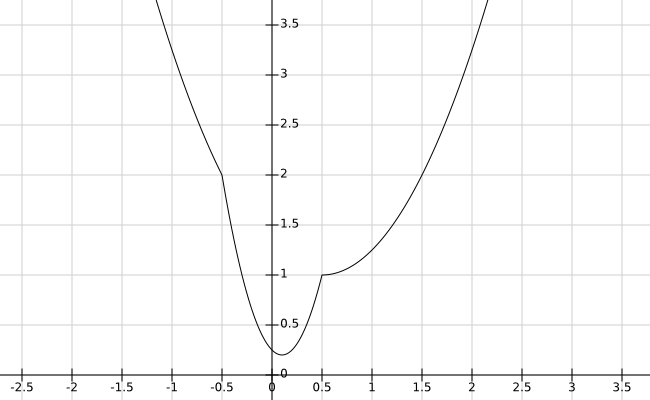
\includegraphics[width=\textwidth]{img/f_1.png}
                        \caption{$(x-\frac{1}{2})^{2} + \min(4x^{2}, 1)$}
                    \end{framed}
                \end{subfigure}
                \begin{subfigure}[b]{0.49\textwidth}
                    \begin{framed}
                        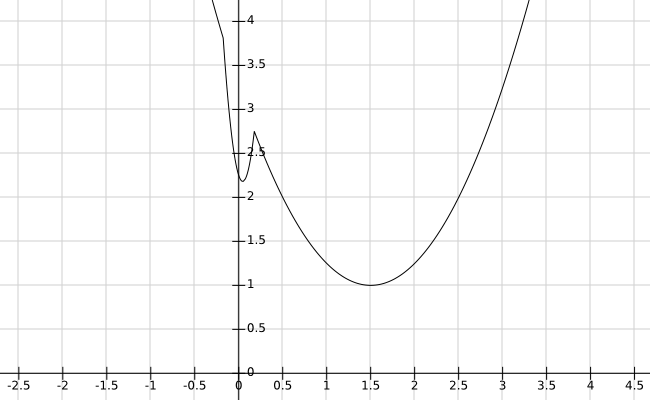
\includegraphics[width=\textwidth]{img/f_2.png}
                        \caption{$(x-\frac{3}{2})^{2} + \min(32x^{2}, 1)$}
                    \end{framed}
                \end{subfigure}
                \begin{subfigure}[b]{0.49\textwidth}
                    \begin{framed}
                        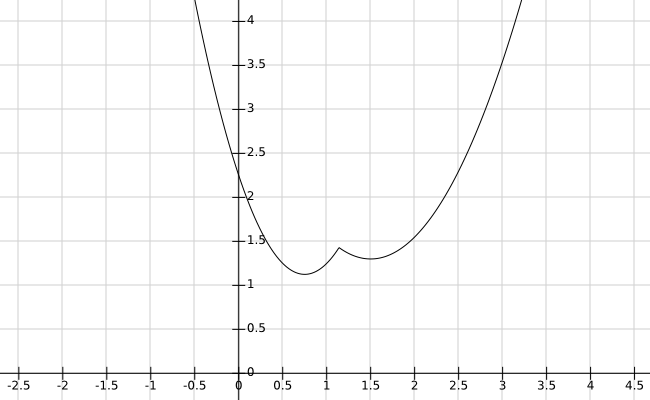
\includegraphics[width=\textwidth]{img/f_4.png}
                        \caption{$(x-\frac{3}{2})^{2} + \min(x^{2}, 1.3)$}
                    \end{framed}
                \end{subfigure}
                \begin{subfigure}[b]{0.49\textwidth}
                    \begin{framed}
                        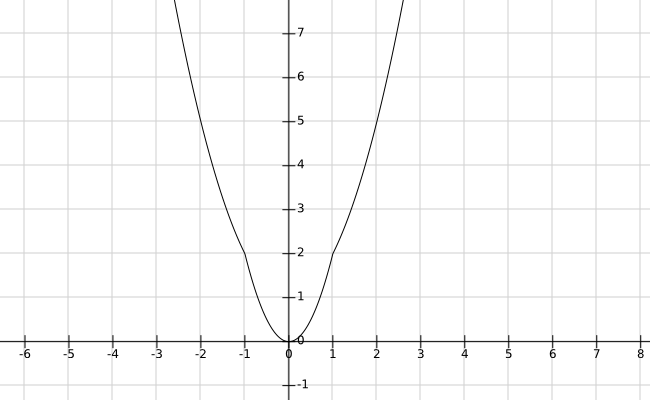
\includegraphics[width=\textwidth]{img/f_5.png}
                        \caption{$x^{2} + \min(x^{2}, 1)$}
                    \end{framed}
                \end{subfigure}
                \caption[Plot of a objective function within a minimum function.]{In (a) and (d) the objective function of the minimization problem only attains one minimum. In (c) we have two minima, but the global minimum is attained for the condition $|\tilde{x}_{i,j}| \le \sqrt{\frac{\nu}{\lambda}(1 + 2\gamma\lambda)}$. In (b) the global minimum is attained in the region in which $|\tilde{x}_{i,j}| > \sqrt{\frac{\nu}{\lambda}(1 + 2\gamma\lambda)}$.}
                \label{fig:objective_function}
            \end{figure}
            According to Strekalovskiy and Cremers in \cite{Strekalovskiy-Cremers-eccv14}, there is no proof of convergence to the minimal value of the Mumford-Shah functional for this framework. Despite that fact, they show the boundedness of $u^{n}$ in the piecewise smooth case. This is summarized in the following proposition.
            \begin{proposition}
                The sequence $(u^{n}, p^{n})$ generated by Algorithm \ref{alg:realtime_primal_dual_algorithm} is bounded and thus compact for $\lambda < \infty$, for instance it has a convergent subsequence.
            \end{proposition}
            The proof can be found in the supplementary material of \cite{Strekalovskiy-Cremers-eccv14}. To determine convergence we also partially follow \cite{Strekalovskiy-Cremers-eccv14} as described in Subsection \ref{sub:stopping_criterion_rof}, but set $\varepsilon = 5 \cdot 10^{-5}$. The difference in our framework is that we evaluate the norm in each iteration step. In \cite{Strekalovskiy-Cremers-eccv14} they compute this norm every ten iteration steps. \\\\
        % subsubsection the_proximity_operators_of_the_tvl1_model (end)
    % section the_mumford_shah_functional (end)
    In this chapter we have provided a framework to solve variational problems, as well as a possibility to minimize the Mumford-Shah functional. In the next chapter we present a second approach to minimize the Mumford-Shah functional.

% chapter convex_optimization_of_the_rof_tvl1_and_mumford_shah_models (end)

\chapter{Minimizing the Mumford-Shah Functional} % (fold)
\label{cha:minimizing_the_mumford_shah_functional}

    As we revisit the Mumford-Shah functional, we also rewrite Definition \ref{def:the_mumford_shah_functional} to be consistent with the publication of Pock, Cremers, Bischof and Chambolle (\cite{Pock-et-al-iccv09}), which we mainly follow in this chapter. If other results are taken into account we point it out.
    \begin{definition}[Mumford-Shah Functional] % (fold)
    \label{def:the_mumford_shah_functional_revisited}
        Let $\Omega \subseteq \mathbb{R}^{2}$ be a rectangular image domain. In order to approximate an input image $f: \Omega \longrightarrow \mathbb{R}$ in terms of a piecewise smooth function $u: \Omega \longrightarrow \mathbb{R}$, the Mumford-Shah functional is defined by
            
            \begin{equation}
                E_{MS}(u) = \lambda \int_{\Omega} (f - u)^{2} dx + \int_{\Omega \setminus S_{u}} |\nabla u|^{2} dx + \nu \mathcal{H}^{1}(S_{u}),
            \label{eq:the_mumford_shah_functional_revisited}
            \end{equation}
        
        where $\lambda, \nu > 0$ are weighting parameters, $S_{u} = S^{1}_{u} \cup ... \cup S^{N}_{u}$ and $\mathcal{H}^{1}(S_{u})$ denotes the one-dimensional Hausdorff-measure of the curves in $S_{u}$. And we seek to minimize $E_{MS}(u)$ over all $u$.
    \end{definition}
    % definition the_mumford_shah_functional (end)
    The difference to Chapter \ref{cha:the_rof_tvl1_and_mumford_shah_functional} is that we interchanged the set $K$ with $S_{u} = S^{1}_{u} \cup ... \cup S^{N}_{u}$ and instead of computing $|K|$, we use the more general notation of measure theory, namely $\mathcal{H}^{1}(S_{u})$. In the case, where $u \in \Omega \subseteq \mathbb{R}^{2}$ the one-dimensional Hausdorff-measure of $S_{u}$ is nothing but $|S_{u}|$. Another difference to Definition \ref{def:the_mumford_shah_functional} is the parameter $\lambda$, which handles the tradeoff between the data fidelity term and the first term in the regularizer. It is swapped and controls the term where the image $f$ enters the functional. This swapping of the parameter also rescales $\nu$ in this formulation. The rescaling does not change the energy, but we need other pairs $(\lambda, \nu)$ for a good image approximation as in the real-time minimzer framework of Subsection \ref{sec:the_mumford_shah_model}. We discuss this issue in Chapter \ref{cha:applications_to_imaging}.\\

    As mentioned in the previous chapter this functional is non-convex. The idea to derive a convex saddle-point representation of the Mumford-Shah functional is to make use of some results presented by Alberti, Bouchitte and Dal Maso.
    \section{Convex Relaxation} % (fold)
    \label{sec:convex_relaxation}
        In order to state a convex representation of the Mumford-Shah functional we introduce the characteristic or level set function.
        \begin{definition}
        \label{def:characteristic_function}
            Let $\Omega \subseteq \mathbb{R}^{2}$ denote the image plane and let $u \in SBV(\Omega)$. The upper level sets of $u$ are denoted by the characteristic function $\mathds{1}_{u}: \Omega \times \mathbb{R} \longrightarrow \{ 0, 1 \}$ of the subgraph of $u$:
                \begin{equation}
                    \mathds{1}_{u}(x, t) =
                        \left\{
                            \begin{array}{l l}
                                1 & \quad \text{if $t < u(x)$} \\
                                0 & \quad \text{else}
                            \end{array}
                        \right. .
                \label{eq:characteristic_function}
                \end{equation}
        \end{definition}
        In Figure \ref{fig:characteristic_function} one can see an example with a characteristic function in $\mathbb{R}^{2}$ for a function $u \in SBV(\Omega)$. So, for a one-dimensional signal $u(x)$ the characteristic function becomes two-dimensional. In our case, as we consider two-dimensional images, the characteristic function ensures that we will act in a three-dimensional space.
        \begin{figure}[!ht]
            \centering
            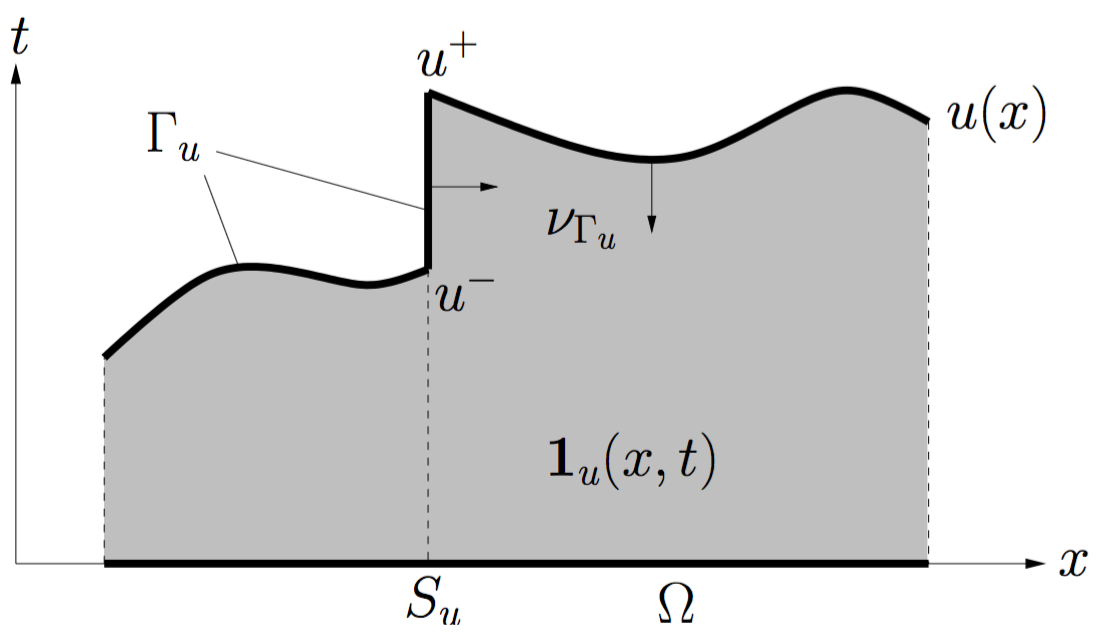
\includegraphics[width=0.7\textwidth]{img/char_func.png}
            \caption[Characteristic Function of a SBV function.]{This picture (taken from \cite{Pock-et-al-iccv09}) shows the characteristic function $\mathds{1}_{u}(x, t)$ of a function $u(x) \in SBV(\Omega)$.}
            \label{fig:characteristic_function}
        \end{figure}
        In Figure \ref{fig:characteristic_function} the gray shaded area is the part where $\mathds{1}_{u}(x, t) = 1$. Otherwise, the characteristic function is set to zero. The upper interface of the gray domain is denoted by $\Gamma_{u}$. This set is the set which holds all parts of the function $u(x)$ and each curve $S_{u}$ connecting the points $u^{-}$ and $u^{+}$. Additionally, the notation $\nu_{\Gamma_{u}}$ denotes the normals on $\Gamma_{u}$.\\

        Using $\mathds{1}_{u}(x, t)$, one can find in \cite{Alberti-et-al-lnss} and \cite{Alberti-et-al-cvpde} the proposed method of Alberti, Bouchitte and Dal Maso to approximate the Mumford-Shah energy by a convex maximization problem. For a proof of this concept we refer to these two publications. We state the theorem in the fashion of \cite{Pock-et-al-iccv09}, which summarizes the results of \cite{Alberti-et-al-lnss} and \cite{Alberti-et-al-cvpde}.
        \begin{theorem}[Convex Relaxation of the Mumford-Shah Functional]
        \label{convex_relaxation_of_the_mumford_shah_functional}
            For a function $u \in SBV(\Omega)$ the Mumford Shah functional can be written as
                \begin{equation}
                    E_{MS}(u) = \sup_{\varphi \in K} \int_{\Omega \times \mathbb{R}} \varphi D\mathds{1}_{u}
                    \label{eq:convex_relaxed_ms}
                \end{equation}
            with a convex set
                \begin{eqnarray}
                    K = \bigg\{ \varphi \in C^{0}(\Omega \times \mathbb{R}, \mathbb{R}^{3}) &:& \varphi^{t}(x, t) \ge \frac{\varphi^{x}(x,t)^{2}}{4} - \lambda(t - f(x))^{2}, \\
                    &&\bigg| \int^{t_{2}}_{t_{1}} \varphi^{x}(x,s)ds \bigg| \le \nu \bigg\}, \label{eq:set_k_continuous}
                \end{eqnarray}
            where the inequalities in the definition of $K$ hold for all $x \in \Omega$ and for all $t, t_{1}, t_{2} \in \mathbb{R}$.
        \end{theorem}
        \begin{remark}
            \begin{itemize}
                \item We used in the theorem that we regard the function $\varphi$ as the representation $\varphi(x, t) = \left( \varphi^{x}(x,t), \varphi^{t}(x,t) \right)^{T}$ where $\varphi(x,t) \in \mathbb{R}^{3}$, $\varphi^{x}(x,t) \in \mathbb{R}^{2}$ and $\varphi^{t}(x,t) \in \mathbb{R}$.
                \item The idea to approximate the Mumford-Shah functional is to maximize the flux of a vector field $\varphi$ through the interface $\Gamma_{u}$. The advantage of this technique is to get a convex representation of the Mumford-Shah functional and for this we derive in the following a convex saddle-point formulation. Then we can - again - make use of the primal-dual algorithm to solve the optimization problem.
                \item Note that $\varphi \in C^{0}(\Omega \times \mathbb{R}, \mathbb{R}^{3})$. In \cite{Pock-et-al-iccv09}, Pock et al. propose $\varphi \in C^{0}(\Omega \times \mathbb{R}, \mathbb{R}^{2})$ which is a typo.
            \end{itemize}
        \end{remark}
        Our goal is to minimize (\ref{eq:convex_relaxed_ms}). We seek to solve
            $$
                \min_{u} E(u) = \min_{u} \left( \sup_{\varphi \in K} \int_{\Omega \times \mathbb{R}} \varphi D\mathds{1}_{u} \right).
            $$
        Following \cite{Pock-et-al-iccv09} we additionally substitute $\mathds{1}_{u}$ by a function
            \begin{equation}
                v(x, t): \Omega \times \mathbb{R} \longrightarrow [0, 1] \,\, \textnormal{and} \,\, \lim_{t \rightarrow -\infty} v(x, t) = 1, \, \, \, \lim_{t \rightarrow +\infty} v(x, t) = 0
            \label{eq:generic_functions}
            \end{equation}
        to compute the minimal energy of the Mumford-Shah functional. Overall, we are going to face the following convex optimization problem:
            \begin{equation}
                \min_{v \in [0, 1]} \sup_{\varphi \in K} \langle v, D\varphi \rangle = \min_{v \in [0, 1]} \sup_{\varphi \in K} \int_{\Omega \times \mathbb{R}} \varphi Dv.
                \label{eq:continous_saddle_point_problem}
            \end{equation}
        According to \cite{Pock-et-al-iccv09} there is no proof that finding an optimal pair $(v^{\ast}, \varphi^{\ast})$ for the optimization problem of (\ref{eq:continous_saddle_point_problem}) leads to the global minimizer of Equation (\ref{eq:the_mumford_shah_functional_revisited}). Further, they state that only if $v^{\ast}$ is binary one gets indeed the global minimum of the Mumford-Shah functional. Despite that fact, solving Equation (\ref{eq:continous_saddle_point_problem}) leads to high-quality approximations $u$ of an input image $f$.
    % section convex_relaxation (end)
    \section{Discrete Setting} % (fold)
    \label{sec:discrete_setting_ms}

        In this section we consider the System (\ref{eq:continous_saddle_point_problem}) in its discrete version. Using the characteristic function and substitute it by the function $v$ means that we are adding an additional space to our two dimensional image domain. This extra label space needs to be considered in the discrete setting. In \cite{Pock-et-al-iccv09} Pock et al. consider $\Omega = [0, 1]^{2}$ and for that the subgraph of $u$ to be in $[0, 1]^{3}$. This would imply that we discretize these two spaces by adding a step-size $h$. Further, they consider all their operators without having this additional step-size. We propose all our spaces and operators without a step size. Then the image domain is defined as $\Omega = \{1, 2, ..., N\} \times \{1, 2, ..., M\}$ and the subgraph of the function $u: \mathbb{R}^{2} \longrightarrow [0, 1]$ is defined in the cube $\Omega \times \{1, 2, ..., S\}$. In this discrete setting we define the pixel grid $\mathcal{G}$ with size $N \times M \times S$ and the following notation
            $$
                \mathcal{G} = \bigg\{ (i , j , k ): i = 1, 2, ..., N, j = 1, ..., M, k = 1, 2, ..., S \bigg\},
            $$
        where $i, j, k$ are the discrete locations of each voxel. For a reformulation of (\ref{eq:continous_saddle_point_problem}) we also need to define the corresponding discrete versions of $v, \varphi$. So, let $u \in X: \mathcal{G} \longrightarrow [0, 1]$ and $p \in Y: \mathcal{G} \longrightarrow \mathbb{R}^{3}$ be the discrete versions of the continuous functions in Equation (\ref{eq:continous_saddle_point_problem}), where $u$ corresponds to $v$ and $p$ to $\varphi$. If we replace the inner-product for infinite dimensions in Equation (\ref{eq:continous_saddle_point_problem}) by the inner-product for finite dimensions, we are going to face the saddle-point problem
            \begin{equation}
                \min_{u \in C} \max_{p \in K} \langle Au, p \rangle.
            \label{eq:mumford_shah_saddle_point_problem}
            \end{equation}
        Here, $A$ is a continuous linear operator, earlier denoted with $K$. Then, this notation looks familiar to us.  And we define the constraint set $C$ by
            \begin{equation}
                C = \{ u \in X: u(i,j,k) \in [0,1], u(i, j, 1) = 1, u(i, j, S) = 0 \}.
            \end{equation}
        In order to take the limits of the function $v$ into account in its discrete version $u$, we set the values in the first label space to $1$ and those in the S-th label space to $0$. According to \cite{Pock-et-al-iccv09} the discrete version of the convex set $K$ from Equation (\ref{eq:set_k_continuous}) has the following representation:
            \begin{eqnarray}
                K = \{ p = (p^{x}, p^{t})^{T} \in Y &:& p^{t}(i,j,k) \ge \frac{||p^{x}(i,j,k)||_{2}^{2}}{4} - \lambda(\frac{k}{S} - f(i,j))^{2}, \label{eq:local_constraint} \\
                &&\left| \sum_{k_{1} \le k \le k_{2}} p^{x}(i,j,k) \right| \le \nu \}, \label{eq:non_local_constraint}
            \end{eqnarray}
        whereas we define $p^{x}(i,j,k) := (p^{1}(i,j,k), p^{2}(i,j,k))^{T}$ and $p^{t}(i,j,k) := p^{3}(i,j,k)$ for a $p(i,j,k) \in \mathbb{R}^{3}$. For this $p = (p^{x}, p^{t}) \in Y \subseteq \mathbb{R}^{N \cdot M \cdot S \cdot 2} \times \mathbb{R}^{N \cdot M \cdot S}$. The constraint in Equation (\ref{eq:local_constraint}) goes pointwise for all $(i, j, k) \in \mathcal{G}$. The second constraint is more involved, since the constraint in (\ref{eq:non_local_constraint}) holds for all $i = 1, ..., N$, $j = 1, ..., M$ and all possible combinations $(k_{1}, k_{2})$ with $1 \le k_{1} \le k \le k_{2} \le S$. What looks like having a set $K$ with two constraints, turns out that the set $K$ is an intersection of a couple of convex sets. One has that for a fixed voxel $(i, j, k)$ one can compute $\frac{S^{2} + S}{2} + 1$ many convex sets. This number rises from the fact that taking into account all possible combinations $(k_{1}, k_{2})$ over all levels $S$ and adding the local-constraint yields
            $$
                \left(\binom{S}{2} + S\right) + 1 = \left(\frac{n!}{k! \cdot (n-k)!} + S\right) + 1 = \left(\frac{S(S-1)}{2} + S\right) + 1 = \frac{S^{2} + S}{2} + 1.
            $$
        The large amount of several convex sets will lead us to a long run-time in the suggested framework of \cite{Pock-et-al-iccv09}. Before we discuss this in detail, we first continue with the definitions of the discrete setting.
        \begin{remark}
            In addition, to discretize the variable $t$ in (\ref{eq:set_k_continuous}) one gets $\frac{k}{S}$ in the discrete version of (\ref{eq:local_constraint}). Note that $t$ is a value in the continuous setting, which determines at which point the characteristic function vanishes. The bound on the norm $L$ depends on the discrete gradient operator, like in Propositions \ref{prop:bound_on_the_norm} and \ref{prop:bound_on_the_norm_ms}. Pock et al. proposed in \cite{Pock-et-al-iccv09} to set the discrete version of $t$ to $\frac{k}{L}$ which is a mistake.
        \end{remark}
        Furthermore, we define the linear operator $A$ in the same fashion as in Section \ref{sec:discrete_setting}, but extended to the additional label space. We have $A = \nabla$ and for that $A^{\ast} = \nabla^{T} = -\textnormal{div}$.
        \begin{definition}[Discrete gradient operator] % (fold)
        \label{def:discrete_gradient_operator_ms}
            We define the discrete gradient operator of $u \in X$ by $\nabla u = ((\partial_{i}u)_{i,j,k}, (\partial_{j}u)_{i,j,k}, (\partial_{k}u)_{i,j,k})^{T}$ using forward differences with Neumann boundary conditions, i.e.
                \begin{eqnarray}
                    &(\partial_{i}u)_{i,j,k} =&
                        \begin{dcases*}
                            u_{i+1, j, k} - u_{i, j, k} & \textnormal{if $i < N$} \\
                            0 & \textnormal{if $i = N$}
                        \end{dcases*},
                    \notag
                    (\partial_{j}u)_{i, j, k} =
                        \begin{dcases*}
                            u_{i, j+1, k} - u_{i, j, k} & \textnormal{if $j < M$} \\
                            0 & \textnormal{if $j = M$}
                        \end{dcases*},
                    \notag \\
                    &(\partial_{k}u)_{i, j, k} =&
                        \begin{dcases*}
                            u_{i, j, k+1} - u_{i, j, k} & \textnormal{if $k < S$} \\
                            0 & \textnormal{if $k = S$}
                        \end{dcases*}.
                    \notag
                \end{eqnarray}
        \end{definition}
        % definition discrete_gradient_operator (end)
        \begin{definition}[Discrete divergence operator] % (fold)
        \label{def:discrete_divergence_operator_ms}
            We define the discrete divergence operator of $p \in Y$ by $\nabla^{T} p = (\partial_{i}p^{1})_{i, j, k} + (\partial_{j}p^{2})_{i, j, k} + (\partial_{k}p^{3})_{i, j, k}$ using backward differences with Dirichlet boundary conditions, i.e.
                \begin{eqnarray}
                    &(\partial_{i}p^{1})_{i, j, k} =&
                        \begin{dcases*}
                            p^{1}_{i, j, k} - p^{1}_{i-1, j, k} & \textnormal{if $1 < i < N$} \\
                            p^{1}_{i, j, k} & \textnormal{if $i = 1$} \\
                            -p^{1}_{i-1, j, k} & \textnormal{if $i = N$}
                        \end{dcases*},
                    \notag
                    (\partial_{j}p^{2})_{i, j, k} =
                        \begin{dcases*}
                            p^{2}_{i, j, k} - p^{2}_{i, j-1, k} & \textnormal{if $1 < j < M$} \\
                            p^{2}_{i, j, k} & \textnormal{if $j = 1$} \\
                            -p^{2}_{i, j-1, k} & \textnormal{if $j = M$}
                        \end{dcases*},
                    \notag \\
                    &(\partial_{k}p^{3})_{i, j, k} =&
                        \begin{dcases*}
                            p^{3}_{i, j, k} - p^{3}_{i, j, k-1} & \textnormal{if $1 < k < S$} \\
                            p^{3}_{i, j, k} & \textnormal{if $k = 1$} \\
                            -p^{3}_{i, j, k-1} & \textnormal{if $k = S$}
                        \end{dcases*}.
                    \notag
                \end{eqnarray}
        \end{definition}
        % definition discrete_gradient_operator (end)
        And we can compute the bound on the norm of $A$, as in Proposition \ref{prop:bound_on_the_norm}.
        \begin{proposition}[Bound on the norm of $\nabla$] % (fold)
            \label{prop:bound_on_the_norm_ms}
            The bound on the norm of the proposed discrete linear operator is given by
                $$
                    L^{2} = ||\nabla||^{2} = ||\nabla^{T}||^{2} \le 12.
                $$
        \end{proposition}
        % proposition bound_on_the_norm (end)
        \begin{proof}
        	The proof remains the same as for Proposition \ref{prop:bound_on_the_norm} by adding the additional discretization variable $p^{3}_{i,j,k}$ and applying Young's inequality thrice with $p = q = 2$.\qed
        \end{proof}

    % section discrete_setting_ms (end)

    \section{Projection onto the sets $\boldsymbol{C}$ and $\boldsymbol{K}$} % (fold)
    \label{sec:projection_onto_the_sets_C_and_K}

        In order to be able to apply the primal-dual algorithm we rewrite Equation \ref{eq:mumford_shah_saddle_point_problem} into
            $$
                \min_{u \in X} \max_{p \in Y} \langle Au, p \rangle - \delta_{K}(p) + \delta_{C}(u).
            $$
        For this we want to evaluate the proximity operators for this framework. As we identify the functions $F^{\ast}(p) = \delta_{K}(p)$ and $G(u) = \delta_{C}(u)$ we know from Example \ref{ex:projection_operator} that the proximity operator of the indicator function is a euclidean projection onto the corresponding set. Before we propose a method to project onto $C$ and $K$, respectively, we rewrite the Primal-Dual Algorithm \ref{alg:primal_dual_algorithm} to be consistent with the work of Pock et al. in \cite{Pock-et-al-iccv09}.
          \begin{algorithm}\label{alg:primal_dual_cremers}
                Choose $(u^{0}, p^{0}) \in C \times K$ and let $\bar{u}^{0} = u^{0}$. We choose $\tau, \sigma > 0$. Then, we let for each $n \ge 0$
                    \begin{equation}
                        \left\{ 
                            \begin{array}{l l}
                              p^{n+1} = \Pi_{K} (p^{n} + \sigma K \bar{u}^{n}) \\
                              u^{n+1} = \Pi_{C} (u^{n} - \tau K^{*} p^{n+1}) \\
                              \bar{u}^{n+1} = 2u^{n+1} - u^{n}
                            \end{array}
                        \right. .
                    \end{equation}
            \end{algorithm}
        We start with the projection onto the set $C$ and go on by providing an algorithm to project onto the set $K$.
        \subsection{Projection onto $\boldsymbol{C}$}
            The projection onto $C$ can efficiently be computed. By definition of the proximity operator we have
                $$
                    u = \arg\min_{u \in X} \frac{||u-\tilde{u}||_{2}^{2}}{2} + \tau \delta_{C}(u) = \arg\min_{u \in C} \sum_{i = 1}^{N} \sum_{j = 1}^{M} \sum_{k = 1}^{S} \frac{|u_{i,j,k} - \tilde{u}_{i,j,k}|^{2}}{2} = \Pi_{C}(\tilde{u}).
                $$
            Assume that $\tilde{u}_{i,j,k} \in C$ for a voxel $(i,j,k)$. Then the best choice for $u_{i,j,k}$ is to set $u_{i,j,k} = \tilde{u}_{i,j,k}$, since the term $|u_{i,j,k} - \tilde{u}_{i,j,k}|^{2}$ is then equal to zero for which the quadratic function is minimal. On the other hand if $\tilde{u}_{i,j,k} \notin C$, the euclidean distance to $C = [0, 1]$ is the shortest distance $\tilde{u}_{i,j,k}$ onto the bound of $C$. This means if $\tilde{u}_{i,j,k} < 0$ then the shortest distance from $\tilde{u}_{i,j,k}$ to $C$ is to set $u_{i,j,k} = 0$. Reversely, if $\tilde{u}_{i,j,k} > 1$ then the euclidean distance to $C$ is given by setting $u_{i,j,k} = 1$. This idea is also illustrated in Figure \ref{fig:projection_onto_c}. For an arbitrary intervall $[a, b]$ we have the following algorithm:
            \begin{algorithm}[Clipping]
                Let $u^{n} \notin [a,b]$ and $a, b \in \mathbb{R}_{\ge 0}$ with $a < b$. The projection of $u^{n}$ onto the interval is given by
                    \begin{equation}
                        u^{n+1} = \min\{b, \max \{ a, u^{n} \} \}
                        \label{eq:clipping}
                    \end{equation}
            \end{algorithm}
            \begin{figure}[!ht]
                \centering
                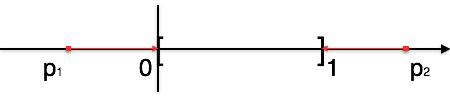
\includegraphics[width=0.9\textwidth]{img/projection_onto_c.png}
                \caption[Clipping on a set.]{A point $p_{1} < 0$ is clipped to $0$, whereas a point $p_{2} > 1$ is clipped to $1$.}
                \label{fig:projection_onto_c}
            \end{figure}
            \begin{remark}
                \label{rem:clipping}
                \begin{itemize}
                    \item By projecting onto $C$, we also need to take care of the limits in (\ref{eq:generic_functions}). For that we set $u(i, j, 1) = 1$ and $u(i, j, S) = 0$ in each projection.
                    \item In the case of our framework - acting in a discrete cube $\mathcal{G}$ - Equation (\ref{eq:clipping}) can be regarded as
                        $$
                            u^{n+1}_{i,j,k} = \min\{1, \max \{ 0, u^{n}_{i,j,k} \} \},
                        $$
                    for all $i = 1, ..., N$, $j = 1, ..., M$ and $k = 1, ..., S$.
                    \item We can easily verify that Equation (\ref{eq:clipping}) is the clipping on the bound of the intervall $[a, b]$. Let $u^{n} < a$, then
                        $$
                            u^{n+1} = \min\{b, \max \{ a, u^{n} \} \} = \min\{b, a\} = a.
                        $$
                    Reversely, we observe for a $u^{n} > b$ that
                        $$
                            u^{n+1} = \min\{b, \max \{ a, u^{n} \} \} = \min\{b, u^{n}\} = b.
                        $$
                \end{itemize}
            \end{remark}
        \subsection{The projection onto $\boldsymbol{K}$} % (fold)
        \label{sub:the_projection_onto_K}
            The projection onto $K$ is more involved, since $K$ takes into account local and non-local constraints. In other words, the set $K$ is an intersection of several convex sets. The projection onto the intersection of convex sets can be done by Dykstra's projection algorithm. The idea behind this algorithm is to project a point $x$ onto each set seperately in an iteration step $n$. Then, as $n \to \infty$ the algorithm finds a point $\hat{x}$ in $K$ for which the distance $||x - \hat{x}||_{2}$ is minimal, see also Figure \ref{fig:dykstra}. The full scheme was first proposed by Boyle and Dykstra in \cite{dykstra-et-al-aors14}, where one can also find a proof of convergence for the proposed algorithm. For more information about Dykstra's projection algorithm, we also refer to \cite{dykstra-et-al-aors14}. We follow the notation of Cremers and Kolev in \cite{Cremers-Kolev-pami11} in our proposed algorithm.
            \begin{figure}[!ht]
                \centering
                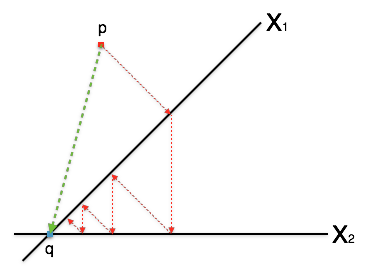
\includegraphics[width=0.5\textwidth]{img/dykstra.png}
                \caption[Dykstra's iteration scheme.]{The point $p$ should be projected onto $q$ which is the point of the intersection of the curves (sets) $X_{1}$ and $X_{2}$. In Dykstra's projection algorithm we alternatingly do euclidean projections onto the corresponding sets $X_{1}$ and $X_{2}$. This is illustrated with the red doted lines.}
                \label{fig:dykstra}
            \end{figure}
            \begin{algorithm}
            \label{alg:dykstra}
                Consider $P$ convex sets $X_{i}$ with $\mathbb{R}^{n} \ni X = X_{1} \cap X_{2} \cap ... \cap X_{P}$. Let $\Pi_{i}$ denote the projection onto the i-th set for $i = 1, ..., P$. And let $u_{c} \in \mathbb{R}^{n}$ be the current estimate with $u_{c} \notin X$, $u_{i}^{k} \in \mathbb{R}^{n}$ for $i = 0, ..., P$ and $v_{i}^{k} \in \mathbb{R}^{n}$ for $i = 1, ..., P$. For $k = 1, 2, ...$ set $u^{0}_{P} = u_{c}$ and $v^{0}_{i} = 0$ for all $i = 1, ..., P$. Then iterate until convergence (e.g. $||u_{0}^{k} - u_{P}^{k}||_{2} \le \varepsilon$ with $\varepsilon$ small):
                \begin{eqnarray}
                    &u_{0}^{k} = &u_{P}^{k-1}, \notag \\
                    &\textnormal{for} \,\, &i = 1, 2, ..., P: \notag \\
                    &&u_{i}^{k} = \Pi_{i}(u_{i-1}^{k} - v_{i}^{k-1}), \notag \\
                    &&v_{i}^{k} = u_{i}^{k} - (u_{i-1}^{k} - v_{i}^{k-1}). \notag
                \end{eqnarray}
            \end{algorithm}
            With this algorithm the projection onto the entire set $K$ can be established. Since the algorithm itself needs the projections onto the constraint sets in each iteration we present how we project onto the subsets of $K$.
        % subsection the_projection_onto_K (end)
        \subsection{Decomposition of $\boldsymbol{K}$} % (fold)
        \label{sub:decomposition_of_K}
            We will decompose the set $K$ into sets $K_{p}$ and $K_{nl}$, where the first resembles the local, or more precisely, a parabola constraint and the second corresponds to the non-local constraint. Overall, we have $K = K_{p} \cap K_{nl}$ with
                $$
                    K_{p} = \left\{ p^{t}(i, j, k) \ge \frac{||p^{x}(i, j, k)||_{2}^{2}}{4} - \lambda(\frac{k}{S} - f(i,j))^{2} \right\},
                $$
            for all $i = 1, ..., N$, $j = 1, ..., M$ and $k = 1, ..., S$. And for the non-local constraint we have
                $$
                    K_{nl} = \left\{ \left| \sum_{k_{1} \le k \le k_{2}} p^{x}(i, j, k) \right| \le \nu \right\},
                $$
            again for all $i = 1, ..., N$ and $j = 1, ..., M$, and in this case for all combinations $(k_{1}, k_{2})$ with $1 \le k_{1} \le k_{2} \le S$. In the following we deduce the projection onto these two sets separately. Let us start with the projection onto the parabola constraint.

        % subsection decomposition_of_K (end)

        \subsection{Projection onto $\boldsymbol{K_{p}}$}
            Since the projection onto the set $K_{p}$ goes pointwise we drop the indices $(i, j, k)$. Note that we do not necessarily need that $p^{x}$ is an element of $\mathbb{R}^{2}$. The following derivation holds for a larger class of problems, namely having $p^{x} \in \mathbb{R}^{n}$. Let $\alpha > 0$, $p^{x} \in \mathbb{R}^{n}$, $p^{t} \in \mathbb{R}$ and $p = (p^{x}, p^{t})^{T} \in \mathbb{R}^{n} \times \mathbb{R}$. Assume that $p_{0}^{t} < \alpha ||p_{0}^{x}||_{2}^{2}$ holds for a point $p_{0} \in \mathbb{R}^{n}\times\mathbb{R}$. Then the projection of $p_{0}$ onto the parabola $\alpha ||p_{0}^{x}||_{2}^{2}$ can be written as the following minimization problem:
                \begin{eqnarray}
                    &\min\limits_{p \in \mathbb{R}^{n} \times \mathbb{R}}& \frac{1}{2} ||p - p_{0}||_{2}^{2} \notag \\
                    &\textnormal{subject to}& p^{t} \ge \alpha||p^{x}||_{2}^{2}. \notag
                \end{eqnarray}
            To find the solution of this optimization problem we introduce a Lagrange multiplier $\mu \in \mathbb{R}$ and define the Lagrangian by
                $$
                    \mathcal{L}(p, \mu) = \frac{||p - p_{0}||_{2}^{2}}{2} - \mu \left( p^{t} - \alpha||p^{x}||_{2}^{2} \right).
                $$
            The minimization problem we consider is convex, because the cost function is convex, the inequality constraint is convex and the feasible set, which is th epigraph of a parabola, is also convex. With this we know that computing a critical point of the Lagrangian function $\mathcal{L}$ also leads to a global optimum of the optimization problem itself. We compute a critical point by
                \begin{equation}
                    \nabla \mathcal{L}(p, \mu) =
                    \begin{pmatrix}
                        \partial_{p^{x}} \mathcal{L}(p, \mu) \\
                        \partial_{p^{t}} \mathcal{L}(p, \mu) \\
                        \partial_{\mu} \mathcal{L}(p, \mu)
                    \end{pmatrix} = 
                    \begin{pmatrix}
                        p^{x} - p_{0}^{x} + \mu 2 \alpha p^{x} \\
                        p^{t} - p_{0}^{t} - \mu \\
                        \alpha||p^{x}||_{2}^{2} - p^{t}
                    \end{pmatrix}
                    = 0. \label{eq:linearSystem}
                \end{equation}
            This means, we need to solve a linear system. In the first equation of (\ref{eq:linearSystem}) we get
                \begin{equation}
                    p_{0}^{x} = (\mu 2 \alpha + 1) p^{x} \iff p^{x} = \frac{p_{0}^{x}}{\mu 2 \alpha + 1}, \label{eq:1stequ}
                \end{equation}
            and the second equation leads us to
                \begin{equation}
                    p^{t} = p_{0}^{t} + \mu. \label{eq:2ndequ}
                \end{equation}
            In the following we discuss two different possibilities how the System (\ref{eq:linearSystem}) can be solved.
            \begin{enumerate}
                \item Inserting the Equalities (\ref{eq:1stequ}) and (\ref{eq:2ndequ}) into the third line of Equation (\ref{eq:linearSystem}) leads us to
                \begin{eqnarray}
                    &&\alpha||p^{x}||_{2}^{2} - p^{t} = 0 \notag \\
                    &\iff& p^{t} - \alpha||p^{x}||_{2}^{2} = 0 \notag \\
                    &\iff& p_{0}^{t} + \mu - \alpha \bigg|\bigg|\frac{p_{0}^{x}}{\mu 2 \alpha + 1}\bigg|\bigg|_{2}^{2} = 0 \notag \\
                    &\iff& p_{0}^{t} + \mu - \frac{\alpha}{(\mu 2 \alpha + 1)^{2}} ||p_{0}^{x}||_{2}^{2} = 0 \notag \\
                    &\overbrace{\iff}^{\cdot (\mu2\alpha + 1)^{2}}& (\mu 2 \alpha + 1)^{2} p_{0}^{t} + (\mu 2 \alpha + 1)^{2} \mu - \alpha ||p_{0}^{x}||_{2}^{2} = 0 \notag \\
                    &\iff& (4 \mu^{2} \alpha^{2} + 4 \mu \alpha + 1) p_{0}^{t} + 4 \mu^{3} \alpha^{2} + 4 \mu^{2} \alpha + \mu - \alpha ||p_{0}^{x}||_{2}^{2} = 0 \notag \\
                    &\iff& 4 \alpha^{2} \mu^{3} + \mu^{2} (4 \alpha^{2} p_{0}^{t} + 4 \alpha) + \mu (4 \alpha p_{0}^{t} + 1) + p_{0}^{t} - \alpha ||p_{0}^{x}||_{2}^{2} = 0. \notag
                \end{eqnarray}
                In order to solve this equation for $\mu$, we define a function
                    $$
                        h(\mu) = 4 \alpha^{2} \mu^{3} + \mu^{2} (4 \alpha^{2} p_{0}^{t} + 4 \alpha) + \mu (4 \alpha p_{0}^{t} + 1) + p_{0}^{t} - \alpha ||p_{0}^{x}||_{2}^{2},
                    $$
                for which we are seeking for the zeroes. Computing the zeroes can efficiently be established by using Newton's algorithm. So, for $k = 1, 2, ...$ compute
                    $$
                        \mu^{k+1} = \mu^{k} - \frac{h(\mu)}{h^{'}(\mu)}.
                    $$
                The first derivative of $h$ is given by
                    $$
                        h^{'}(\mu) = 12 \alpha^{2} \mu^{2} + 2 \mu (4 \alpha^{2} p_{0}^{t} + 4 \alpha) + (4 \alpha p_{0}^{t} + 1).
                    $$
                Overall, we get the update equation for a $\mu^{k+1}$ with
                    $$
                        \mu^{k+1} = \mu^{k} - \frac{4 \alpha^{2} \mu^{3} + \mu^{2} (4 \alpha^{2} p_{0}^{t} + 4 \alpha) + \mu(4 \alpha p_{0}^{t} + 1) + p_{0}^{t} - \alpha ||p_{0}^{x}||_{2}^{2}}{12 \alpha^{2} \mu^{2} + 2 \mu (4 \alpha^{2} p_{0}^{t} + 4 \alpha) + (4 \alpha p_{0}^{t} + 1)}.
                    $$
                In \cite{Chambolle-et-al-10}, Chambolle et al. suggested to set $\mu^{0} = \max \{ 0, - \frac{2 p_{0}^{t}}{3} \}$, where they state that Newton's method converges within 7-10 iterations to a quite accurate solution. With Equations (\ref{eq:1stequ}) and (\ref{eq:2ndequ}) and the computed value for $\mu$ we are able to evaluate $p$ by
                    $$
                        p = \left( \frac{p_{0}^{x}}{\mu 2 \alpha + 1}, p_{0}^{t} + \mu \right).
                    $$
                We do not suggest using this method, since the primal-dual algorithm will be extremely slow in the case of this framework. Having a few iterations of Newton's algorithm in each primal-dual iteration, additionally generates more overhead and for that would decelerate the program. Further, Newton's method is inexact and as it turns out, the second approach to this problem will lead to an exact solution which can be computed within one loop of straightforward computations.
                \item For the second approach we note that (\ref{eq:1stequ}) and (\ref{eq:2ndequ}) hold and plug these equalities into the third equation in (\ref{eq:linearSystem}) which can then be expressed by
                    \begin{equation}
                        p^{t} = \alpha ||p^{x}||_{2}^{2} \iff p_{0}^{t} + \mu = \alpha ||p^{x}||_{2}^{2}. \label{eq:tmp1}
                    \end{equation}
                With Equation (\ref{eq:1stequ}) we can compute the solution of $\mu$ by
                    \begin{eqnarray}
                        p^{x} = \frac{p_{0}^{x}}{\mu 2 \alpha + 1} &\iff& ||p^{x}||_{2} = \bigg|\bigg| \frac{p_{0}^{x}}{1 + 2 \alpha \mu} \bigg|\bigg|_{2} \notag \\
                        &\iff& ||p^{x}||_{2} = \frac{1}{1 + 2 \alpha \mu} ||p_{0}^{x}||_{2} \notag \\
                        &\iff& \frac{1}{1 + 2 \alpha \mu} = \frac{||p^{x}||_{2}}{||p_{0}^{x}||_{2}} \notag \\
                        &\iff& 1 + 2\alpha\mu = \frac{||p_{0}||_{2}}{||p_{x}||_{2}} \notag \\
                        &\iff& 2 \alpha \mu = \frac{||p_{0}^{x}||_{2}}{||p^{x}||_{2}} - 1 \notag \\
                        &\iff& \mu = \frac{1}{2 \alpha} \left( \frac{||p_{0}^{x}||_{2}}{||p^{x}||_{2}} \right) - \frac{1}{2\alpha}. \notag
                    \end{eqnarray}
                We insert the solution of $\mu$ into (\ref{eq:tmp1}) and observe
                    \begin{eqnarray}
                        &&\alpha ||p^{x}||_{2}^{2} = p_{0}^{t} + \frac{1}{2 \alpha} \left( \frac{||p_{0}^{x}||_{2}}{||p^{x}||_{2}} \right) - \frac{1}{2\alpha} \notag \\
                        &\overbrace{\iff}^{\cdot 2 \alpha ||p^{x}||_{2}}& 2 \alpha^{2} ||p^{x}||_{2}^{3} = 2 \alpha p_{0}^{t} ||p^{x}||_{2} + ||p_{0}^{x}||_{2} - ||p^{x}||_{2} \notag \\
                        &\iff& 2 \alpha^{2} ||p^{x}||_{2}^{3} + ||p^{x}||_{2} - 2\alpha p_{0}^{t} ||p^{x}||_{2} - ||p_{0}^{x}||_{2} = 0. \notag \\
                        &\iff& 2 \alpha^{2} ||p^{x}||_{2}^{3} + (1 - 2 \alpha p_{0}^{t}) ||p^{x}||_{2} - ||p_{0}^{x}||_{2} = 0. \notag \\
                        &\overbrace{\iff}^{\cdot 4 \alpha}& 8 \alpha^{3} ||p^{x}||_{2}^{3} + 4 \alpha (1 - 2 \alpha p_{0}^{t}) ||p^{x}||_{2} - 4 \alpha ||p_{0}^{x}||_{2} = 0. \notag \\
                        &\iff& (2 \alpha ||p^{x}||_{2})^{3} + 2 (1 - 2 \alpha p_{0}^{t}) 2 \alpha ||p^{x}||_{2} - 4 \alpha ||p_{0}^{x}||_{2} = 0. \notag \\
                        &\iff& t^{3} + 3bt - 2a = 0, \label{eq:cubic}
                    \end{eqnarray}
                with $a = 2 \alpha ||p_{0}^{x}||_{2}$, $b = \frac{2}{3}(1 - 2 \alpha p_{0}^{t})$ and $t = 2 \alpha ||p^{x}||_{2}$.\\
                The cubic Equation (\ref{eq:cubic}) in $t$ can efficiently be solved using the analytical formula for solving cubic equations published by J. P. McKelvey in 1984 in \cite{kelvey-ajp}.
            \end{enumerate}
            The result of McKelvey's publication is summarized in the following algorithm. Note that we already computed the factors $a$ and $b$. The other factors follow with \cite{kelvey-ajp}. We propose our algorithm in the fashion of \cite{strekalovskiy-et-al-siims14}.
                \begin{algorithm}
                    \label{alg:projection_on_parabola}
                    Let $\alpha > 0, p_{0}^{t} \in \mathbb{R}, p_{0}^{x} \in \mathbb{R}^{n}$. If $p_{0}^{t} \ge \alpha ||p_{0}^{x}||_{2}^{2}$ is already satisfied set $(p^{x}, p^{t}) = (p_{0}^{x}, p_{0}^{t})$. Otherwise, with $a = 2 \alpha ||p_{0}^{x}||_{2}$, $b = \frac{2}{3} (1 - 2 \alpha p_{0}^{t})$, and
                        \[
                            d =
                                \begin{dcases*}
                                    a^{2} + b^{3} & \textnormal{if $b \ge 0$}\\
                                    (a - \sqrt{-b}^{3})(a + \sqrt{-b}^{3}) & \textnormal{else}
                                \end{dcases*},
                        \]
                    set
                        \[
                            v =
                                \begin{dcases*}
                                    c - \frac{b}{c} \,\, \textnormal{with} \,\, c = \sqrt[3]{a + \sqrt{d}} & \textnormal{if $d \ge 0$}\\
                                    2 \sqrt{-b} \cos \left( \frac{1}{3} \arccos \frac{a}{\sqrt{-b}^{3}} \right) & \textnormal{else}
                                \end{dcases*}.
                        \]
                    If $c = 0$ in the first case, set $v = 0$. The solution is then given by
                        \[
                            p^{x} =
                                \begin{dcases*}
                                    \frac{v}{2\alpha} \frac{p_{0}^{x}}{||p_{0}^{x}||_{2}} & \textnormal{if $p_{0}^{x} \ne 0$}\\
                                    0 & \textnormal{else}
                                \end{dcases*},
                        \]
                    and $p^{t} = \alpha ||p^{x}||_{2}^{2}$.
                \end{algorithm}
            The above method states that the projection onto the parabola can be done by one cycle of straightforward computations. The implementation of it is simple and the algorithm has a fast run-time. It is only left to show, how we project onto $K_{nl}$.

        \subsection{Projection onto $K_{nl}$}
            \label{sub:projection_onto_K_nl}

            The set $K_{nl}$ is a combination of non-local constraints, meaning that in a fixed pair $(i,j)$ we sum up all possible combinations of $p^{x}(i,j,k)$ for all $1 \le k_{1} \le k \le k_{2} \le S$. So, we can not project pointwise. Let us assume that we consider a vector $p \in \mathbb{R}^{S \times 2}$ at a fixed pair $(i,j)$. We denote $p$ by $p = (p^{x}_{1}, p^{x}_{2}, ..., p^{x}_{S})$, where $p^{x}_{k} \in \mathbb{R}^{2}$ for all $k = 1, ..., S$. Further, we consider a fixed pair $(k_{1}, k_{2})$ with $1 \le k_{1} \le k_{2} \le S$. The set $K_{nl}$ is therefore defined as
                $$
                    K_{nl} = \left\{ \left| \sum_{k_{1} \le k \le k_{2}} p^{x}_{k} \right| \le \nu \right\}.
                $$
            The projection of a vector $\tilde{p} \in \mathbb{R}^{S \times 2}$ for a fixed pair $(k_{1}, k_{2})$ onto the set $K_{nl}$ can be expressed by the following optimization problem:
                \begin{subequations}
                    \begin{align}
                    \min\limits_{p \in \mathbb{R}^{2 \times S}} &\frac{1}{2} ||p - \tilde{p}||^{2}_{2} \label{eq:equalityConstraint} \\
                    \textnormal{subject to} \,\,\, &\left| \sum_{k_{1} \le k \le k_{2}} p^{x}_{k} \right| \le \nu. \label{eq:inequalityConstraint}
                    \end{align}
                    \label{eq:optimization_problem}
                \end{subequations}
            We seek to find the minimal distance of $\tilde{p}$ to $K_{nl}$ by additionally fulfilling the inequality constraint in (\ref{eq:inequalityConstraint}). Then, the following algorithm establishes the projection of a $\tilde{p}$ onto $K_{nl}$ for a fixed pair $(k_{1}, k_{2})$.
            \begin{algorithm}[Soft-Shrinkage Scheme]
            \label{alg:softshrinkage}
                Choose $\tilde{p}, p \in \mathbb{R}^{S \times 2}$, $\tilde{p}_{k}, p_{k} \in \mathbb{R}^{2}$ for all $k = 1, ..., S$ and choose a pair $(k_{1}, k_{2})$, such that $1 \le k_{1} \le k_{2} \le S$. If $\tilde{p} \notin K_{nl}$ use $\tilde{s}_{k_{1}, k_{2}}, s_{k_{1}, k_{2}} \in \mathbb{R}^{2}$ and compute $\tilde{s}_{k_{1}, k_{2}} = \sum_{k_{1} \le k \le k_{2}} \tilde{p}^{x}_{k}$ together with
                    $$
                        s_{k_{1}, k_{2}} =
                            \begin{dcases*}
                                \tilde{s}_{k_{1}, k_{2}} & \textnormal{if $|\tilde{s}_{k_{1}, k_{2}}| \le \nu$}\\
                                \frac{\nu}{|\tilde{s}_{k_{1}, k_{2}}|} \tilde{s}_{k_{1}, k_{2}} & \textnormal{else}
                            \end{dcases*}.
                    $$
                Then, iterate for all $k = 1, .., S$ and set
                    \begin{equation}
                        p^{x}_{k} =
                            \begin{dcases*}
                                \tilde{p}^{x}_{k} + \frac{s_{k_{1}, k_{2}} - \tilde{s}_{k_{1}, k_{2}}}{k_{2} - k_{1} + 1} & \textnormal{if $k_{1} \le k \le k_{2}$} \\
                                \tilde{p}^{x}_{k} & \textnormal{else}
                            \end{dcases*}.
                        \label{eq:softshrinkage}
                    \end{equation}
                If $\tilde{p}$ already satisfies the inequality constraint (\ref{eq:inequalityConstraint}) or equivalently $\tilde{p} \in K_{nl}$, set $p = \tilde{p}$.
            \end{algorithm}
            \begin{proposition}
                \label{prop:softshrinkage}
                The solution generated in Equation (\ref{eq:softshrinkage}) by Algorithm \ref{alg:softshrinkage}, solves the optimization problem (\ref{eq:optimization_problem}) optimally.
            \end{proposition}
            To prove this proposition, we make use of the Karush-Kuhn-Tucker optimality conditions of Theorem \ref{the:kkt_conditions}.
            \begin{proof}
            For fixed pairs $(i,j)$ and $(k_{1}, k_{2})$ let $\tilde{p} \in \mathbb{R}^{S \times 2}$ and let $\tilde{s}_{k_{1}, k_{2}}, s_{k_{1}, k_{2}} \in \mathbb{R}^{2}$ be as in Algorithm \ref{alg:softshrinkage}. If $\tilde{p}$ already satisfies the inequality constraint in \ref{eq:inequalityConstraint}, which means that $\tilde{p} \in K_{nl}$, we set $p^{\ast} = \tilde{p}$ as the solution of System (\ref{eq:optimization_problem}). With this choice the quadratic function in (\ref{eq:equalityConstraint}) is zero and for that minimal.

            For the rest of the proof we assume that $\tilde{p} \notin K_{nl}$ and for this also $\tilde{s} \neq 0$, since $\nu > 0$. We know from Example \ref{ex:convex_function} 1. that a quadratic function, e.g. (\ref{eq:equalityConstraint}), is strictly convex. This implies that if we find a local solution of System (\ref{eq:optimization_problem}), it is already a global solution.

            Relating to the inequality constraint in (\ref{eq:inequalityConstraint}) we define a function $c: \mathbb{R}^{S \times 2} \to \mathbb{R}$ by
                $$
                    c(p) = \frac{1}{2} \nu^{2} - \frac{1}{2} \left| \sum_{k_{1} \le k \le k_{2}} p^{x}_{k} \right|^{2}.
                $$
            Suppose $p^{\ast} \in \mathbb{R}^{S \times 2}$ is the unique solution of System (\ref{eq:optimization_problem}) and we characterize $p^{\ast}$ by $p^{\ast}_{k} = \tilde{p}_{k} + \frac{s_{k_{1}, k_{2}} - \tilde{s}_{k_{1}, k_{2}}}{k_{2} - k_{1} + 1}$ if $k_{1} \le k \le k_{2}$ and $p^{\ast}_{k} = \tilde{p}_{k}$ else. For this $p^{\ast}$, we can show that the constraint in (\ref{eq:inequalityConstraint}) is active:
                \begin{eqnarray}
                    c(p^{\ast}) &=& \frac{1}{2} \nu^{2} - \frac{1}{2} \bigg|\sum_{k_{1} \le k \le k_{2}} p^{\ast}_{k}\bigg|^{2} \notag \\
                    &=& \frac{1}{2} \nu^{2} - \frac{1}{2} \bigg|\sum_{k_{1} \le k \le k_{2}} \left( \tilde{p}_{k} + \frac{s_{k_{1}, k_{2}} - \tilde{s}_{k_{1}, k_{2}}}{k_{2} - k_{1} + 1} \right) \bigg|^{2} \notag \\
                    &=& \frac{1}{2} \nu^{2} - \frac{1}{2} \bigg| \underbrace{\sum_{k_{1} \le k \le k_{2}} \tilde{p}_{k}}_{= \tilde{s}_{k_{1}, k_{2}}} + \underbrace{\sum_{k_{1} \le k \le k_{2}} \frac{s_{k_{1}, k_{2}} - \tilde{s}_{k_{1}, k_{2}}}{k_{2} - k_{1} + 1}}_{= (k_{2} - k_{1} + 1) \left(\frac{s_{k_{1}, k_{2}} - \tilde{s}_{k_{1}, k_{2}}}{k_{2} - k_{1} + 1}\right)} \bigg|^{2} \label{eq:long_formula} \\
                    &=& \frac{1}{2} \nu^{2} - \frac{1}{2} \underbrace{|s_{k_{1}, k_{2}}|^{2}}_{= \nu^{2}} = 0 \label{eq:short_formula}
                \end{eqnarray}
            Now, we want to show that LICQ holds at $p^{\ast}$. Let us first evaluate the gradient of the function $c$ in $p^{\ast}$. We observe
                $$
                    \nabla c(p^{\ast}) =
                    \begin{pmatrix}
                            0 \\
                            \vdots \\
                            0 \\
                            - \sum\limits_{k_{1} \le k \le k_{2}} p^{\ast}_{k} \\
                            \vdots \\
                            - \sum\limits_{k_{1} \le k \le k_{2}} p^{\ast}_{k} \\
                            0 \\
                            \vdots \\
                            0
                        \end{pmatrix},
                $$
            and we consider the i-th row for which $k_{1} \le i \le k_{2}$ and compute
                $$
                    (\nabla c(p^{\ast}))_{i} = - \sum_{k_{1} \le k \le k_{2}} \left( \tilde{p}_{k} + \frac{s_{k_{1}, k_{2}} - \tilde{s}_{k_{1}, k_{2}}}{k_{2} - k_{1} + 1} \right) = -s,
                $$
            where we used the equality of Equations (\ref{eq:long_formula}) and (\ref{eq:short_formula}). The gradient of $c$ in $p^{\ast}$ is then given by
                $$
                    \nabla c(p^{\ast}) =
                    \begin{pmatrix}
                            0 \\
                            \vdots \\
                            0 \\
                            - s \\
                            \vdots \\
                            - s \\
                            0 \\
                            \vdots \\
                            0
                        \end{pmatrix}.
                $$
            Since $\tilde{s} \neq 0$ it follows that $s \neq 0$ by definition of $s$ and $\nabla c(p^{\ast})$ is linear independent. It is left to show that there is a Lagrange multiplier $\lambda^{\ast} \in \mathbb{R}$ such that the KKT conditions hold for $(p^{\ast}, \lambda^{\ast})$. For this we first define the Lagrange function by
                $$
                    \mathcal{L}(p, \lambda) = \frac{1}{2} ||p - \tilde{p}||_{2}^{2} - \lambda \left( \frac{1}{2} \nu^{2} - \frac{1}{2} \left| \sum_{k_{1} \le k \le k_{2}} p_{k} \right|^{2} \right).
                $$
            We evaluate $\nabla \mathcal{L}(p^{\ast}, \lambda^{\ast})$ and observe
                $$
                    \nabla \mathcal{L}(p^{\ast}, \lambda^{\ast}) =
                        \begin{pmatrix}
                            p^{\ast}_{1} - \tilde{p}_{1} \\
                             \\
                             \\
                            \vdots \\
                            \vdots \\
                            \vdots \\
                             \\
                             \\
                            p^{\ast}_{S} - \tilde{p}_{S}
                        \end{pmatrix}
                    - \lambda^{\ast} \begin{pmatrix}
                            0 \\
                            \vdots \\
                            0 \\
                            - \sum_{k_{1} \le k \le k_{2}} p^{\ast}_{k} \\
                            \vdots \\
                            - \sum_{k_{1} \le k \le k_{2}} p^{\ast}_{k} \\
                            0 \\
                            \vdots \\
                            0
                        \end{pmatrix} =
                        \begin{pmatrix}
                            p^{\ast}_{1} - \tilde{p}_{1} \\
                             \\
                             \\
                            \vdots \\
                            \vdots \\
                            \vdots \\
                             \\
                             \\
                            p^{\ast}_{S} - \tilde{p}_{S}
                        \end{pmatrix}
                    + \lambda^{\ast} \begin{pmatrix}
                            0 \\
                            \vdots \\
                            0 \\
                            s \\
                            \vdots \\
                            s \\
                            0 \\
                            \vdots \\
                            0
                        \end{pmatrix}.
                $$
                If we consider the i-th row of $\nabla \mathcal{L}(p^{\ast}, \lambda^{\ast})$ with $i < k_{1}$ or $i > k_{2}$ then we have that $\lambda^{\ast}$ can be chosen arbitrarily, because
                    $$
                        p^{\ast}_{i} - \tilde{p}_{i} + \lambda^{\ast} \cdot 0 = 0 \iff  p^{\ast}_{i} = \tilde{p}_{i}.
                    $$
                In order to compute $\lambda^{\ast}$ we need to consider the i-th row of $\nabla \mathcal{L}(p^{\ast}, \lambda^{\ast})$ for which $i$ satisfies $k_{1} \le i \le k_{2}$. We observe
                    \begin{eqnarray}
                        &&p^{\ast}_{i} - \tilde{p}_{i} + \lambda^{\ast} s = 0 \notag \\
                        &\iff& \left(\tilde{p}_{i} + \frac{s_{k_{1}, k_{2}} - \tilde{s}_{k_{1}, k_{2}}}{k_{2} - k_{1} + 1}\right) - \tilde{p}_{i} + \lambda^{\ast}  = 0 \notag \\
                        &\iff& \frac{s_{k_{1}, k_{2}} - \tilde{s}_{k_{1}, k_{2}}}{k_{2} - k_{1} + 1} + \lambda^{\ast}s_{k_{1}, k_{2}} = 0 \notag \\
                        &\overset{s = \frac{\nu}{|\tilde{s}_{k_{1}, k_{2}}|}\tilde{s}_{k_{1}, k_{2}}}{\iff}& \frac{\frac{\nu}{|\tilde{s}_{k_{1}, k_{2}}|} \tilde{s}_{k_{1}, k_{2}} - \tilde{s}_{k_{1}, k_{2}}}{k_{2} - k_{1} + 1} + \lambda^{\ast}\frac{\nu}{|\tilde{s}_{k_{1}, k_{2}}|} \tilde{s}_{k_{1}, k_{2}} = 0 \notag \\
                        &\iff& \tilde{s}_{k_{1}, k_{2}} \left( \frac{\frac{\nu}{|\tilde{s}_{k_{1}, k_{2}}|} - 1}{k_{2} - k_{1} + 1} + \lambda^{\ast}\frac{\nu}{|\tilde{s}_{k_{1}, k_{2}}|} \right) = 0 \notag
                    \end{eqnarray}
                Since $\tilde{s}_{k_{1}, k_{2}} \neq 0$ and $|\tilde{s}_{k_{1}, k_{2}}| > \nu$, we can evaluate $\lambda^{\ast}$ by
                    \begin{eqnarray}
                        && \frac{\frac{\nu}{|\tilde{s}_{k_{1}, k_{2}}|} - 1}{k_{2} - k_{1} + 1} + \lambda^{\ast}\frac{\nu}{|\tilde{s}_{k_{1}, k_{2}}|} = 0 \notag \\
                        &\iff& \lambda^{\ast}\frac{\nu}{|\tilde{s}_{k_{1}, k_{2}}|} = \frac{1 - \frac{\nu}{|\tilde{s}_{k_{1}, k_{2}}|}}{k_{2} - k_{1} + 1} \notag \\
                        &\iff& \lambda^{\ast} = \underbrace{\frac{1}{k_{2} - k_{1} + 1}}_{> 0} \left( \underbrace{\frac{|\tilde{s}_{k_{1}, k_{2}}|}{\nu}}_{> 1} - 1 \right) > 0. \notag
                    \end{eqnarray}
                For this $\lambda^{\ast} > 0$, the gradient of $\mathcal{L}(p^{\ast}, \lambda^{\ast})$ vanishes. Because the inequality constraint is active at $p^{\ast}$, the complementary slackness condition is satisfied. According to the work of Stephen Boyd and Lieven Vandenberghe (\cite{Boyd}, page 244) we know as our optimization problem is convex that the KKT conditions are already sufficient conditions and we proved Proposition \ref{prop:softshrinkage}.\qed
            \end{proof}
    We presented methods to project onto the sets $C$ and $K$. In order to project onto $K$, by using Dykstra's projection algorithm, we showed how projections onto the subsets of $K$ can efficiently be computed. As we will see in Chapter \ref{cha:applications_to_imaging}, this approach needs a huge amount of memory and is extremely slow, even on a GPU. In the next section we present an alternative approach which yields a faster computation time.
    % section projection_on_the_sets_C_and_K (end)
    \section{An Alternative Approach using Lagrange Multiplier} % (fold)
    \label{sec:an_alternative_approach_using_lagrangre_multipliers}
        
        In this section we present an alternative formulation of the saddle-point problem in Equation (\ref{eq:mumford_shah_saddle_point_problem}). This approach also solves the convex relaxed Mumford-Shah functional and is orders of magnitudes faster as the previously presented approach. In this framework the projections onto $C$ and $K_{p}$ remain unchanged, but the difference is that we get rid of Dykstra's projection algorithm to save computation time. In order to derive such a representation we decouple $K_{nl}$ and introduce Lagrange multipliers. We will obtain another saddle-point problem which can then be solved with a modified version of the primal-dual algorithm. In the original problem
            \begin{equation}
                \min_{u \in C} \max_{p \in K} \langle Au, p \rangle,
                \label{eq:original_saddle_point_problem}
            \end{equation}
        we maximized over the whole set $K$ defined in Equations (\ref{eq:local_constraint}) and (\ref{eq:non_local_constraint}). In order to rewrite this formulation we revisit the non-local constraint set defined in the fashion of Subsection \ref{sub:projection_onto_K_nl}, by
            $$
                K_{nl} = \left\{ \left| \sum_{k_{1} \le k \le k_{2}} p^{x}_{k} \right| \le \nu \right\},
            $$
        at all possible positions $(i,j)$ for all $i = 1, ..., N$, $j = 1, ..., M$ and all combinations $(k_{1}, k_{2})$ with $1 \le k_{1} \le k_{2} \le S$. Decoupling of $K_{nl}$ then means that we substitute $\sum_{k_{1} \le k \le k_{2}} p^{x}_{k}$ by $s_{k_{1}, k_{2}}$ and introduce an additional constraint to take the bound on $\nu$ into account. We have
            \begin{equation}
                K_{nl} = \left\{ |s_{k_{1}, k_{2}}| \le \nu \,\,\, \textnormal{subject to} \,\,\, s_{k_{1}, k_{2}} = \sum_{k_{1} \le k \le k_{2}} p^{x}_{k} \right\},
                \label{eq:non_local_constraint_reloaded}
            \end{equation}
        again for all pairs $(i,j)$, all combinations $1 \le k_{1} \le k \le k_{2} \le S$, $s_{k_{1}, k_{2}} \in \mathbb{R}^{2}$ and $s \in \mathbb{R}^{N \times M \times I \times 2}$. Here, $I = \frac{S^{2} + S}{2}$ denotes the number of all non-local constraint sets. We further present an auxiliary variable $\mu_{k_{1}, k_{2}} \in \mathbb{R}^{2}$, which belongs to a $\mu \in \mathbb{R}^{N \times M \times I \times 2}$ and define a Lagrange function
            \begin{equation}
                \mathcal{L}(u, \mu, p, s) = \langle Au, p \rangle + \sum_{k_{1} = 1}^{S} \sum_{k_{2} = k_{1}}^{S} \langle \mu_{k_{1}, k_{2}}, \sum_{k_{1} \le k \le k_{2}} p^{x}_{k} - s_{k_{1}, k_{2}} \rangle,
                \label{eq:lagrangian}
            \end{equation}
        in which we added an enforced term to our original problem corresponding to the constraint in $K_{nl}$. Taking into account that the constraint in (\ref{eq:non_local_constraint_reloaded}) is an equality constraint we have that $\mu_{k_{1}, k_{2}} \in \mathbb{R}^{2}$ for all $1 \le k_{1} \le k_{2} \le S$. Using the Lagrangian in (\ref{eq:lagrangian}) we have the following proposition:
            \begin{proposition}
                \label{prop:equivalence_of_two_problems}
                Let $(u^{\ast}, p^{\ast})$ be the solution of (\ref{eq:original_saddle_point_problem}) and $(u^{\ast}, \mu^{\ast}, p^{\ast}, s^{\ast})$ be the solution of
                    \begin{equation}
                        \min_{\substack{u \in C \\ \mu_{k_{1}, k_{2}}}} \max_{\substack{p \in K_{p} \\ |s_{k_{1}, k_{2}}| \le \nu}} \mathcal{L}(u, \mu, p, s).
                        \label{eq:lagrange_saddle_point_problem}
                    \end{equation}
                Then, the equality
                    \begin{equation}
                        \langle Au^{\ast}, p^{\ast} \rangle = \mathcal{L}(u^{\ast}, \mu^{\ast}, p^{\ast}, s^{\ast})
                        \label{eq:equality_of_problems}
                    \end{equation}
                holds.
            \end{proposition}
            \begin{proof}
                Let $u^{\ast}, \mu^{\ast}, p^{\ast}, s^{\ast}$ be the optimal values of Equations (\ref{eq:original_saddle_point_problem}) and (\ref{eq:lagrange_saddle_point_problem}).\\
                We show $\langle Au^{\ast}, p^{\ast} \rangle \ge \mathcal{L}(u^{\ast}, \mu^{\ast}, p^{\ast}, s^{\ast})$. Then we observe the inequality
                    \begin{eqnarray}
                        \mathcal{L}(u^{\ast}, \mu^{\ast}, p^{\ast}, s^{\ast}) &=& \min_{\substack{u \in C \\ \mu_{k_{1}, k_{2}}}} \max_{\substack{p \in K_{p} \\ |s_{k_{1}, k_{2}}| \le \nu}} \langle Au, p \rangle + \sum_{k_{1} = 1}^{S} \sum_{k_{2} = k_{1}}^{S} \langle \mu_{k_{1}, k_{2}}, \sum_{k_{1} \le k \le k_{2}} p^{x}_{k} - s_{k_{1}, k_{2}} \rangle \notag \\
                        &\le& \min_{\substack{u \in C \\ \mu_{k_{1}, k_{2}}}} \langle Au, p^{\ast} \rangle + \sum_{k_{1} = 1}^{S} \sum_{k_{2} = k_{1}}^{S} \langle \mu_{k_{1}, k_{2}}, \sum_{k_{1} \le k \le k_{2}} p^{\ast^{x}}_{k} - s^{\ast}_{k_{1}, k_{2}} \rangle \label{eq:before_cases} \\
                        &=& \begin{dcases*}
                            \langle Au^{\ast}, p^{\ast} \rangle, & \textnormal{if $\sum\limits_{k_{1} \le k \le k_{2}} p^{\ast^{x}}_{k} = s^{\ast}_{k_{1}, k_{2}}$} \\
                            -\infty & \textnormal{else}
                        \end{dcases*} \label{eq:cases} \\
                        &\le& \langle Au^{\ast}, p^{\ast} \rangle. \notag
                    \end{eqnarray}
                In Equality (\ref{eq:cases}) we used that if $\sum_{k_{1} \le k \le k_{2}} p^{\ast^{x}}_{k} = s^{\ast}_{k_{1}, k_{2}}$, the last term in (\ref{eq:before_cases}) vanishes. But, if $\sum_{k_{1} \le k \le k_{2}} p^{\ast^{x}}_{k} \neq s^{\ast}_{k_{1}, k_{2}}$ the minimum over all $\mu$ assures that the last term in (\ref{eq:before_cases}) tends to $-\infty$.\\
                Let us now show $\langle Au^{\ast}, p^{\ast} \rangle \le \mathcal{L}(u^{\ast}, \mu^{\ast}, p^{\ast}, s^{\ast})$: If $p^{\ast}$ is the optimal value of Equation (\ref{eq:original_saddle_point_problem}) it also satisfies $p^{\ast} \in K = K_{p} \cap K_{nl}$. But this implies $p^{\ast} \in K_{p}$ and $p^{\ast} \in K_{nl}$ and for that we can set $s^{\ast}_{k_{1}, k_{2}} = \sum_{k_{1} \le k \le k_{2}} p^{\ast^{x}}_{k}$ for all possible pairs $(k_{1}, k_{2})$. Then, we compute
                    \begin{eqnarray}
                        \langle Au^{\ast}, p^{\ast} \rangle &=& \min_{u \in C} \max_{\substack{p \in K_{p} \\ p \in K_{nl}}} \langle Au, p \rangle \notag \\
                        &\le& \min_{u \in C} \langle Au, p^{\ast} \rangle \notag \\
                        &=& \min_{\substack{u \in C \\ \mu_{k_{1}, k_{2}}}} \langle Au, p^{\ast} \rangle + \sum_{k_{1} = 1}^{S} \sum_{k_{2} = 1}^{S} \langle \mu_{k_{1}, k_{2}}, \underbrace{\sum_{k_{1} \le k \le k_{2}} p^{\ast^{x}}_{k} - s^{\ast}_{k_{1}, k_{2}}}_{= 0} \rangle \notag \\
                        &=& \mathcal{L}(u^{\ast}, \mu^{\ast}, p^{\ast}, s^{\ast}). \notag
                    \end{eqnarray}\qed 
            \end{proof}
        As discussed in Section \ref{sec:the_general_saddle_point_problem}, doing a gradient descent in the primal and a gradient ascent in the dual variable simultaneously means that we need to estimate the direction of the steepest descent and ascent, respectively. For that we compute $\nabla \mathcal{L}(u, \mu, p, s)$ and use the partial derivatives with respect to $u, \mu, p$ and $s$ in the corresponding update equations of the primal-dual algorithm. We compute
            \begin{eqnarray}
                \frac{\partial \mathcal{L}(u, \mu, p, s)}{\partial u} &=& A^{T} p \\
                \frac{\partial \mathcal{L}(u, \mu, p, s)}{\partial s_{k_{1}, k_{2}}} &=& -\sum_{k_{1} = 1}^{S} \sum_{k_{2} = 1}^{S} \mu_{k_{1}, k_{2}} \\
                \frac{\partial \mathcal{L}(u, \mu, p, s)}{\partial \mu_{k_{1}, k_{2}}} &=& \sum_{k_{1} = 1}^{S} \sum_{k_{2} = 1}^{S} \left( \sum_{k_{1} \le k \le k_{2}} p^{x}_{k} - s_{k_{1}, k_{2}} \right) \\
                \frac{\partial \mathcal{L}(u, \mu, p, s)}{\partial p} &=& Au + \hat{p}.
            \end{eqnarray}
        As a last step we need to estimate $\hat{p}$. We therefore consider the partial derivative in the l-th component in the direction of $p$.
            \begin{eqnarray}
                \frac{\partial \mathcal{L}(u, \mu, p, s)}{\partial p_{l}} &=& (Au)_{l} + \frac{\partial}{\partial p_{l}} \left(\sum_{k_{1} = 1}^{S} \sum_{k_{2} = k_{1}}^{S} \langle \mu_{k_{1}, k_{2}}, \sum_{k_{1} \le k \le k_{2}} p^{x}_{k} - s_{k_{1}, k_{2}} \rangle \right) \notag \\
                &=& (Au)_{l} + \frac{\partial}{\partial p_{l}} \left(\sum_{k_{1} = 1}^{S} \sum_{k_{2} = k_{1}}^{S} \left( \langle \mu_{k_{1}, k_{2}}, \sum_{k_{1} \le k \le k_{2}} p^{x}_{k} \rangle - \langle \mu_{k_{1}, k_{2}}, s_{k_{1}, k_{2}} \rangle \right) \right) \notag \\
                &=& (Au)_{l} + \frac{\partial}{\partial p_{l}} \left(\sum_{k_{1} = 1}^{S} \sum_{k_{2} = k_{1}}^{S} \langle \mu_{k_{1}, k_{2}}, \sum_{k_{1} \le k \le k_{2}} p^{x}_{k} \rangle \right) \notag \\
                &=& (Au)_{l} + 
                    \begin{pmatrix}
                        \sum\limits_{k_{1} = 1}^{l} \sum\limits_{k_{2} = l}^{S} \mu_{k_{1}, k_{2}}^{1} \\
                        \sum\limits_{k_{1} = 1}^{l} \sum\limits_{k_{2} = l}^{S} \mu_{k_{1}, k_{2}}^{2} \\
                        0
                    \end{pmatrix}.\notag
            \end{eqnarray}
        With this it follows
            $$
                \tilde{p} =
                    \begin{pmatrix}
                        \sum\limits_{k_{1} = 1}^{l} \sum\limits_{k_{2} = l}^{S} \mu_{k_{1}, k_{2}}^{1} \\
                        \sum\limits_{k_{1} = 1}^{l} \sum\limits_{k_{2} = l}^{S} \mu_{k_{1}, k_{2}}^{2} \\
                        0
                    \end{pmatrix}.
            $$
        Recalling that we computed $I = \frac{S^{2} + S}{2}$, having these four updates and setting $A = \nabla$, we observe a new formulation for our primal-dual algorithm by:\newpage
            \begin{algorithm}
                \label{alg:mumford_shah_lagrange_multiplier}
                Choose $(u^{0}, p^{0}, \mu^{0}, s^{0}) \in C \times K_{p} \times \mathbb{R}^{2 \times N \times M \times I} \times \mathbb{R}^{2 \times N \times M \times I}$ and let $\bar{u}^{0} = u^{0}, \bar{\mu}^{0} = \mu^{0} = 0, p^{0} = 0$. Set $\tau_{u} = \frac{1}{6}, \tau_{\mu} = \frac{1}{150}, \sigma_{p} = \frac{1}{3 + S}, \sigma_{s} = 1$. Then, we let for each $n \ge 0$
                    \begin{equation}
                        \left\{ 
                            \begin{array}{l l}
                              p^{n+1} = \Pi_{K_{p}} \left(p^{n} + \sigma_{p} (A \bar{u}^{n} + \tilde{p})\right) \\
                              s_{k_{1}, k_{2}}^{n+1} = \Pi_{|\cdot| \le \nu} \left(s_{k_{1}, k_{2}}^{n} - \sigma_{s} \left( \sum_{k_{1} = 1}^{S} \sum_{k_{2} = 1}^{S} \bar{\mu}_{k_{1}, k_{2}}^{n} \right) \right) \\
                              u^{n+1} = \Pi_{C} \left(u^{n} - \tau_{u} A^{*} p^{n+1} \right) \\
                              \mu_{k_{1}, k_{2}}^{n+1} = \mu_{k_{1}, k_{2}}^{n} + \tau_{\mu} \left( \sum_{k_{1} \le k \le k_{2}} p^{x}_{k} - s_{k_{1}, k_{2}}^{n+1} \right) \\
                              \bar{u}^{n+1} = 2u^{n+1} - u^{n} \\
                              \bar{\mu}_{k_{1}, k_{2}}^{n+1} = 2\mu_{k_{1}, k_{2}}^{n+1} - \mu_{k_{1}, k_{2}}^{n}.
                            \end{array}
                        \right.
                    \end{equation}
            \end{algorithm}
        Once implemented this variant of the primal-dual algorithm derives the same approximation as the ordinary primal-dual algorithm using Dykstra's projection algorithm in each iteration step. The big difference between the two frameworks is the performance. We discuss this in Chapter \ref{cha:applications_to_imaging}. In the following we additionally show how the approximation $u$ can be extracted from the three-dimensional space into a two-dimensional object.
    \section{Computing the 0.5-Isosurface} % (fold)
    \label{sec:computing_the_0_5_isosurface}

        By using convex relaxation methods for minimizing the Mumford-Shah functional, we compute the approximation $u$ in a three-dimensional space. So, we need a framework to extract the two-dimensional approximation $\hat{u}$. Therefore, we compute the 0.5-isosurface. The idea is to interpolate the corresponding channel at each pixel position $(i,j)$ for $k = 1, ..., S$ by thresholding at $0.5$. Before we propose the whole procedure, let us first explain how the interpolation with a threshold at $0.5$ can be derived.
        \begin{remark}[Linear Newton Interpolation]
            Recalling the linear Newton interpolation scheme, we can compute a function $u(x)$ by a convex combination of two pairs $(x_{0}, u(x_{0}))$ and $(x_{1}, u(x_{1}))$. The formula is given by
                $$
                    u(x) = u(x_{0}) + \frac{u(x_{1} - u(x_{0}))}{x_{1} - x_{0}}\left( x - x_{0} \right).
                $$
        \end{remark}
        The idea is to iterate for all $k = 1, ..., S$ at a fixed pair $(i,j)$, until we find a value at the position $x_{0} = \frac{k}{S}$ which fulfills the strict inequality $u(x_{0}) > 0.5$ and additionally find a value $x_{1} = \frac{k+1}{S}$ together with $u(x_{1}) \le 0.5$. Then, we can compute the function $u$ at $0.5$, namely $u(0.5)$, using Newton's linear interpolation formula by
            \begin{eqnarray}
                u(0.5) &=& \frac{k}{S} + \frac{\frac{k+1}{S} - \frac{k}{S}}{x_{1} - x_{0}} \left( 0.5 - x_{0} \right) \notag \\
                &=& \frac{k}{S} + \frac{1}{S} \frac{0.5 - x_{0}}{x_{1} - x_{0}} \notag \\
                &=& \frac{1}{S} \left( k + \frac{0.5 - x_{0}}{x_{1} - x_{0}} \right). \notag
            \end{eqnarray}
        Overall, we propose the following algorithm for computing the 0.5-isosurface:
        \begin{algorithm}[0.5-isosurface]
            \label{alg:0.5_isosurface}
            Let $(i,j)$ be a fixed pair of all locations $i = 1, ..., N$ and $j = 1,..., M$. Iterate from $1, ..., S-1$ and evaluate $u(i,j,k)$ and $u(i,j,k+1)$, until
                $$
                    u(i,j,k) > 0.5 \,\,\, \textnormal{and} \,\,\, u(i,j,k+1) \le 0.5,
                $$
            and set
                $$
                    \hat{u}(i,j) = \frac{1}{S} \left( k + \frac{0.5 - u(i,j,k)}{u(i,j,k+1) - u(i,j,k)} \right).
                $$
            If we do not find such a pair, we set
                $$
                    \hat{u}(i,j) = u(i, j, S).
                $$
            Then $\hat{u}$ denotes the two-dimensional approximation of the input image $f$.
        \end{algorithm}
    % section computing_the_0_5_isosurface (end)
    \section{Convergence Criterion} % (fold)
    \label{sec:convergence_criterion}
    
        As a convergence criterion we adapted the idea of the real-time minimizer framework. But we need to take into account that $u$ is a three-dimensional object in the underlying algorithm. This means we need to modify the stopping criterion. We evaluate once every ten iterations
            $$
                ||u^{n+1} - u^{n}|| \le \varepsilon,
            $$
        with $\varepsilon = 5 \cdot 10^{-5}$. Then, the norm is computed by
            $$
                ||\tilde{u}|| = \frac{1}{N \cdot M \cdot S} \sum_{i = 1}^{N} \sum_{j = 1}^{M} \sum_{k = 1}^{S} |\tilde{u}_{i,j,k}|.
            $$
        If we consider color images, we need a fourth loop over all $l = 1, 2, 3$ to take all color channels into account.\\

    % section stopping_criterion (end)

    In this chapter we proposed a method for minimizing the Mumford-Shah functional. We rewrote the minimzation into a saddle-point problem to be able to use the primal-dual algorithm. Additionally, we presented two frameworks how the proposed saddle-point problem can be solved. The suggested method in \cite{Pock-et-al-iccv09}, namely using Dykstra's projection algorithm to project onto the set $K$, is extremely slow, as Chapter \ref{cha:applications_to_imaging} reveals. Decoupling of the set $K$ into $K_{p}$ and $K_{nl}$ and applying a Lagrange multiplier formalism led to a reformulation of the original saddle-point problem, for which we also rewrote the primal-dual algorithm. As we will see in Chapter \ref{cha:applications_to_imaging}, this approach is far more applicable and leads to a better run-time.

% chapter minimizing_the_mumford_shah_functional (end)

\chapter{Applications to Imaging} % (fold)
\label{cha:applications_to_imaging}

    In this chapter we present applications to imaging for the proposed models. We consider image cartooning by using the real-time minimizer for the Mumford-Shah model. This framework together with the ROF and TVL1 model are taken into account, when we show image denoising. A modified version of the ROF model is applicable for image inpainting. At the end of this chapter we compare the two approaches for minimizing the convex relaxed Mumford-Shah functional, namely using Dykstra's projection algorithm and the Lagrange multiplier method. We also show that the Mumford-Shah is the most edge preserving method of all proposed models and good in image segmentation.

    \section{General Setting} % (fold)
    \label{sec:general_setting}
        
        We present several results in this chapter for image approximation, denoising, inpainting and image segmentation. We run all our tests on two different computers. The serial code is implemented on a CPU (Central Processing Unit) using the programming language C++. We execute the code on a MacBook Air (13-inch, Early 2014) with a 1,4 GHz Intel Core i5 Processor and a 4 GB 1600 MHz DDR3 internal memory. The two approaches for minimizing the convex relaxed Mumford-Shah functional needed parallelization to be applicable. In order to the implementation of both approaches we additionally parallelized our serial code on a GPU (Graphical Processor Unit) using the Nvidia CUDA framework. For more information on CUDA we refer to \cite{CUDA}. The code is executed at the University of Regensburg on the RZ411 computer containing a Nvidia Quadro K4000 GPU running 64-bit Rex-Linux. We additionally made use of the OpenCV library to read and write images in all our implementations. We refer to \cite{OpenCV} for more information on OpenCV.\\
        In the following sections we also present code examples for the primal-dual algorithm in C++. These examples are not the actual functions we use in our program. They are just a possible implementation we propose in this thesis. Further, we will not provide CUDA examples in this thesis, because it would go beyond the scope. For our complete coding, including the CUDA implementation, we refer to our computer program iPaur (image Processing At University of Regensburg) found on Github (\cite{Bauer}).\\
        In Figure \ref{fig:images_used} we show the used images in our tests. The images (a) to (d) are images of Lena (or Lenna) Soderberg. We degraded the original Lena image in (a) with five percent Gaussain noise and twenty-five percent salt and pepper noise, respectively, in (b) and (c). And we removed seventy percent of the data in image (d). The images (g) to (i) are taken from the publication of Pock et al. in \cite{Pock-et-al-iccv09}. Let us mentioned that the Ladama image is originally called La Dama con l'ermellino and a painting by Leonardo da Vinci. The Synthetic Test image of (h) is further degraded with five percent Gaussian noise, seen in (i). The other two color valued images in (e) and (f) are taken from the Github repository online at \cite{FastMS}. This repository belongs to the publication of Strekalovskiy and Cremers in \cite{Strekalovskiy-Cremers-eccv14}.\\
        \begin{figure}[!ht]
                \centering
                \begin{subfigure}[b]{0.24\textwidth}
                    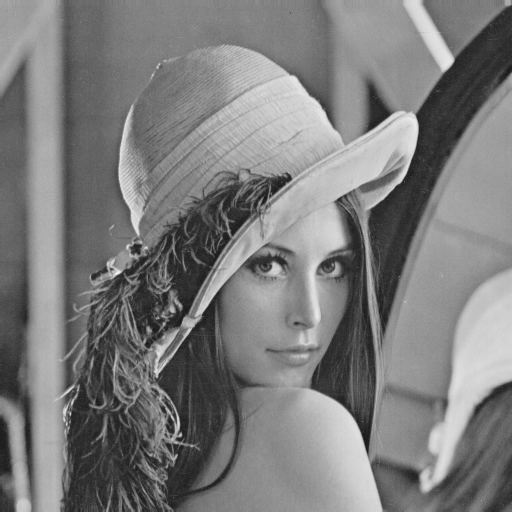
\includegraphics[width=\textwidth]{img/images/lena.png}
                    \caption{Lena image.}
                \end{subfigure}
                \begin{subfigure}[b]{0.24\textwidth}
                    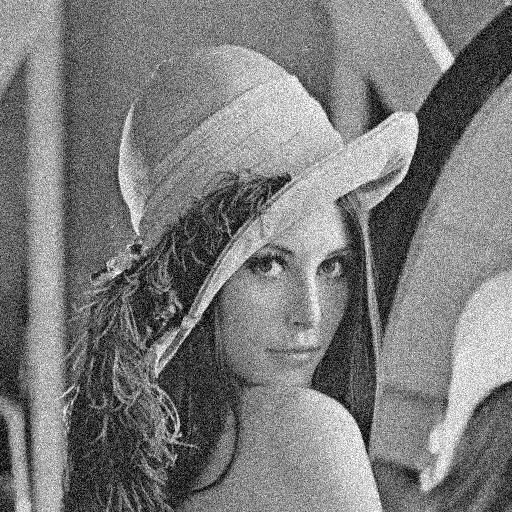
\includegraphics[width=\textwidth]{img/images/lena_gauss_noise.png}
                    \caption{Gaussian noise.}
                \end{subfigure}
                \begin{subfigure}[b]{0.24\textwidth}
                    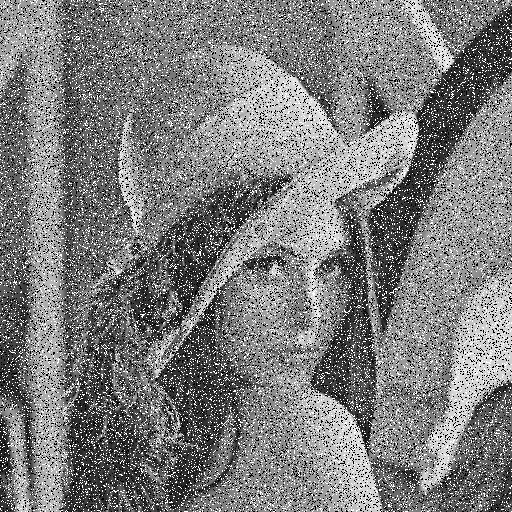
\includegraphics[width=\textwidth]{img/images/lena_sp_noise.png}
                    \caption{S. \& P. noise.}
                \end{subfigure}
                \begin{subfigure}[b]{0.24\textwidth}
                    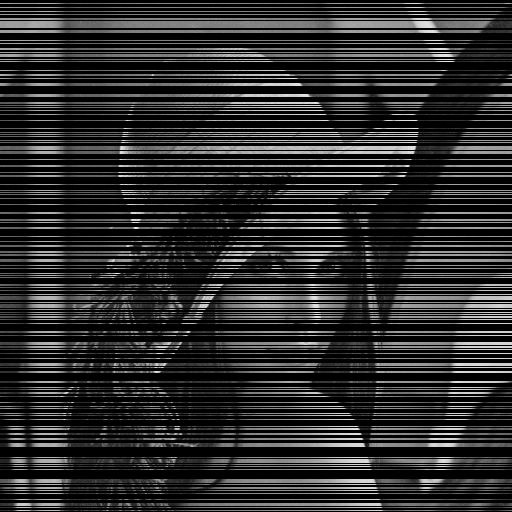
\includegraphics[width=\textwidth]{img/images/lena_inpaint.png}
                    \caption{Data loss.}
                \end{subfigure}
                \begin{subfigure}[b]{0.4\textwidth}
                    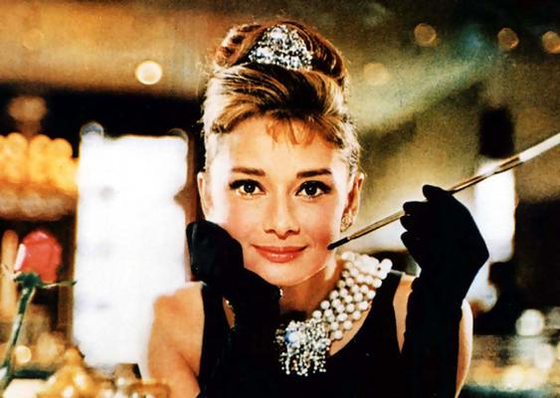
\includegraphics[width=\textwidth]{img/images/hepburn.png}
                    \caption{Audrey Hepburn Image.}
                \end{subfigure}
                \begin{subfigure}[b]{0.425\textwidth}
                    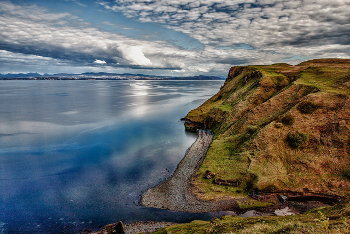
\includegraphics[width=\textwidth]{img/images/landscape.png}
                    \caption{Landscape image.}
                \end{subfigure}
                \begin{subfigure}[b]{0.3\textwidth}
                    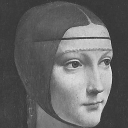
\includegraphics[width=\textwidth]{img/images/ladama.png}
                    \caption{Ladama image.}
                \end{subfigure}
                \begin{subfigure}[b]{0.3\textwidth}
                    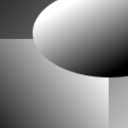
\includegraphics[width=\textwidth]{img/images/synth.png}
                    \caption{Synthetic Test image.}
                \end{subfigure}
                \begin{subfigure}[b]{0.3\textwidth}
                    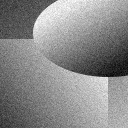
\includegraphics[width=\textwidth]{img/images/synth_gauss_noise.png}
                    \caption{Gaussian noise.}
                \end{subfigure}
                \caption[Images used in Chapter 5]{(a) - (d) are grayscaled images with a size of $512 \times 512$. (g) - (i) are also grayscaled images with a size of $128 \times 128$. (e) is an RGB image of size $560 \times 398$ and (f) an RGB image of size $350 \times 234$.}
            \label{fig:images_used}
            \end{figure}
        
        We additionally introduce two important formulae used in the following sections. They can also be found in the book of Kristian Bredies and Dirk Lorenz in \cite{Bredies}.\newpage
        \begin{definition}[MSE and PSNR]
            Let $u, v \in \mathbb{R}^{N \times M}$ be two discrete images. Then the MSE is given by
                \begin{equation}
                    MSE(u,v) = \frac{1}{NM} \sum_{i = 1}^{N} \sum_{j = 1}^{M} (u_{i,j} - v_{i,j})^{2}.
                    \label{eq:mse}
                \end{equation}
            If $u_{i,j}, v_{i,j} \in [0, 255]$, then we define the peak-signal-noise-ratio (PSNR) by
                \begin{equation}
                    PSNR(u, v) = 10 \log_{10} \left( \frac{255^{2}}{MSE(u,v)} \right)\, \textnormal{db}.
                    \label{eq:psnr}
                \end{equation}
        \end{definition}
        The PSNR is used to compare the difference between two images, given in decibel. It is a scaling of the MSE and measures the possible maximal energy of an image $u$ to the energy of the image $v$ degraded with noise. If we derive a PSNR over $40$ for two images $u,v$ the human eye can not distinguish between the images $u$ and $v$. For more information on this, we refer to \cite{Bredies}.\\
        To the end of this section let us mention some technical details on the programming language C++ and the examples we provide. From now on we let the number of color channels be determined by $B$. So, in the case of grayscaled images $B = 1$ and for color valued images, here RGB images, $B = 3$. Furthermore, we provide our functions as templated functions. This means that we do not determine the data type of our vectors beforehand. For more information on the C++ programming language and templating we refer to \cite{CPlusPlus}. As a last thing we mention that if we have an array of length $n$ the indices in C++ start at $0$ and end at $n-1$.
    % section general_setting (end)

    \section{Linearized Storage of Images} % (fold)
    \label{sec:linearized_storage_of_images}
        
        In this section we show how images are stored ideally. Images in a discrete two-dimensional grid $\mathcal{G}$ of size $N \times M$ can be viewed as matrices. The first element is stored at the top left corner. Then, the next entries are stored row-wise from the left to the right side. The last element of this matrix is then at the bottom right. To save computation time we do not store two-dimensional images in matrix form, but use a linearized version. In a programming language like C++, an image $u$ in matrix form would be accessed with
            $$
                u[i][j] = value,
            $$
        where $i$ resembles the i-th row and $j$ the j-th column. We store all data in one vector, so we allocate a vector $u$ of the size $N \cdot M$ and attach each line of the matrix to this array. Then we access elements by
            $$
                u[j + i \cdot M] = value.
            $$
        This method works well for grayscaled images if we map from the discret pixel grid $\mathcal{G}$ (see also Equation (\ref{eq:pixel_grid})) for instance to $[0, 1]$ or $\{ 0, ..., 255 \}$. Note, $g, u$ and $\hat{u}$ in the proposed primal-dual algorithm are stored in this fashion. In the case of color images, here RGB (red-green-blue) images, we can extend this kind of linearized storage easily. For that, we assume that each single color channel has its own pixel grid. We have for $k = 1, ..., B$
            \begin{equation}
                \mathcal{G}_{k} = \bigg\{ (i, j) : i = 1, ..., N \,\, \textnormal{and} \,\, j = 1, ..., M \bigg\}.
                \label{eq:color_pixel_grid}
            \end{equation}
        Overall, we attach each channel with its grid separately to the vectors consecutively. Then, we have $u \in \mathbb{R}^{N \cdot M \cdot B}$ and access one element with $k = 1, ..., B$, by
            $$
                u[j + i \cdot M + k \cdot M \cdot N] = value.
            $$
        Furthermore, we need to consider the variables $p$ in the primal-dual algorithm. These are also stored as vectors, but with the extension that for a fixed point $(i, j, k)$ we have $p_{i,j,k} \in \mathbb{R}^{2}$. We have two possibilities how to handle the storage of these variables. The way we choose is to allocate two vectors of the size $N \cdot M \cdot B$ and call them $p_{x}$ and $p_{y}$, respectively.
        Another possibility is to do the same as before: attach the values of $p_{y}$ to these of $p_{x}$ and observe one large array which can be accessed by
            $$
                p[j + i \cdot M + k \cdot M \cdot N + l \cdot M \cdot N \cdot B] = value,
            $$
        with $l = 1, 2$ or for grayscaled images
            $$
                p[j + i \cdot M + l \cdot M \cdot N] = value.
            $$
        For us, it seemed to be necessary to use the first method for obtaining a readable and maintainable code. With this setting we are ready to present the first considered model: The ROF model.
    % section linearized_storage_of_images (end)

    \section{Image Approximation using the ROF Model} % (fold)
    \label{sec:image_approximation_using_the_rof_model}
        
        In this section we show approximations of input images. Besides we show how the primal-dual algorithm can be implemented efficiently and estimate well fitting parameters for this model.

        \subsection{Implementation Issues} % (fold)
        \label{sub:implementation_issues}
            
            In our framework we implemented the ROF model in C++ on a CPU and GPU. Since the serial code is quite fast we consider the serial version in this section, but also provide run-times of the parallelized version. We set $K = \nabla$ with the proposed discretization stated in Section \ref{sec:discrete_setting}. Further, we consider each vector, e.g. $u$ or $\bar{u}$, being accessed with $u_{i,j,k}$. For the approximation of color images we have that $k = 1, .., B$, in the case of grayscaled images $k = B = 1$. Further, we allocate the vectors $u, \bar{u}, g \in [0,255]^{B}$ and $p_{x}, p_{y} \in \mathbb{R}$. And we suggest to initialize $\bar{u} = u = g$ and $p_{x} = p_{y} = 0$ in the primal-dual algorithm.

            \subsubsection{Computing $p^{n+1} = (\textnormal{Id} + \sigma\,\partial\,F^{\ast})^{-1}(p^{n} + \sigma\,\nabla\bar{u}^{n})$}
            \label{sub:computing_p}

                In each iteration step we need to estimate the gradient of $\bar{u}^{n}$. For this we allocate two variables $dx$ and $dy$ at a given point $(i,j,k)$ and compute under the premise that we discretized $\nabla$ by forward differences with Neumann boundary conditions
                    $$
                        dx = \bar{u}_{i+1,j,k} - \bar{u}_{i,j,k} \,\,\,\,\, \textnormal{and} \,\,\,\,\, dy = \bar{u}_{i,j+1,k} - \bar{u}_{i,j,k},
                    $$
                where we set $dx = 0$ if $i + 1 < N$ and $dy = 0$ if $j + 1 < M$.
                After that, we multiply both values with $\sigma$ and then add the old estimate of $p$, namely $p_{x}^{n}$ and $p_{y}^{n}$ to $dx$ and $dy$, respectively. This means
                    $$
                        dx = p_{x_{i,j,k}}^{n} + \sigma * dx \,\,\,\,\, \textnormal{and} \,\,\,\,\, dy = p_{y_{i,j,k}}^{n} + \sigma * dy.
                    $$
                At the end we need to apply the proximity operator of the function $F^{\ast}$ to the variables $dx$ and $dy$ and save the observed value in $p_{i,j,k}^{n+1}$. We compute
                    $$
                        p_{x_{i,j,k}}^{n+1} = \frac{dx}{\max(1, norm)} \,\,\,\,\, \textnormal{and} \,\,\,\,\, p_{y_{i,j,k}}^{n+1} = \frac{dy}{\max(1, norm)},
                    $$
                where $norm = \sqrt{dx*dx+dy*dy}$. Then a dual ascent function could look as follows:
                \begin{lstlisting}
template<typename T>
void dual_asc(T* p_x, T* p_y, T* u_bar, T sigma, int M, int N, int B) {
  T dx, dy, norm;
  int index;
  for (int k = 0; k < B; k++) {
    for (int i = 0; i < N; i++) {
      for (int j = 0; j < M; j++) {
        index = j + i * M + k * N * M;
        dx = i+1<N ? u_bar[j + (i+1) * M + k * N * M]-u_bar[index] : 0;
        dy = j+1<M ? u_bar[(j+1) + i * M + k * N * M]-u_bar[index] : 0;
        dx = p_x[index] + sigma * dx;
        dy = p_y[index] + sigma * dy;
        norm = sqrt(dx*dx+dy*dy);
        p_x[index] = dx / max(1.f, norm);
        p_y[index] = dy / max(1.f, norm);
      }
    }
  }
}
                \end{lstlisting}
            These few lines of code are used to compute the update on $p_{i,j,k}^{n+1}$ for all $i = 1, ..., N$, $j = 1, ..., M$ and $k = 1, ... B$. To be able to use this function in another framework, e.g. for minimizing the TVL1 energy, we only need to exchange the last three lines in the inner for-loops, resembling the proximity operator for $F^{\ast}$.

            \subsubsection{Computing $u^{n+1} = (\textnormal{Id} - \tau\,\partial\,G)^{-1}(u^{n} + \tau\,\nabla^{T}p^{n+1})$}
            \label{sub:computing_u}

                Again, we allocate values $dx$, $dy$ and additionally $sum$, in which we store the sum of the partial derivatives. Note, that we change the minus sign in front of the transposed nabla operator, since $K^{\ast} = \nabla^{T}$ is defined as the negative divergence operator. Using backward differences with Dirichlet boundary conditions, like in Definition \ref{def:discrete_divergence_operator}, we compute
                    $$
                        dx = p_{x_{i,j,k}} - p_{x_{i-1,j,k}} \,\,\, \textnormal{and} \,\,\, dy = p_{y_{i,j,k}} - p_{y_{i,j-1,k}} \,\,\, \textnormal{and} \,\,\, sum = \tau \cdot (dx + dy).
                    $$
                We additionally take into account that if $i + 1 < N$ or $j + 1 < M$, we have
                    $$
                        dx = -p_{x_{i-1,j,k}} \,\,\,\,\, \textnormal{or} \,\,\,\,\, dy = -p_{y_{i,j-1,k}}
                    $$
                and if $i > 0$ or $j > 0$, we compute
                    $$
                        dx = p_{x_{i,j,k}} \,\,\,\,\, \textnormal{or} \,\,\,\,\, dy = p_{y_{i,j,k}}.
                    $$
                As we already multiplied the discrete divergence with the parameter $\tau$ we further add the previous estimate $u_{i,j,k}^{n}$ by
                    $$
                        sum = u_{i,j,k}^{n} + sum.
                    $$
                In a last step we apply the proximity operator for the function $G$ and observe
                    $$
                        u_{i,j,k}^{n+1} = \frac{sum + \tau\lambda g_{i,j,k}}{1 + \tau\sigma}.
                    $$
                The primal descent function could then be implemented in the following fashion:
                    \begin{lstlisting}
template<typename T>
void primal_desc(T* p_x, T* p_y, T* u, T* g, T tau, T lambda, int M, int N, int B) {
  T dx, dy, sum;
  int index;
  for (int k = 0; k < B; k++) {
    for (int i = 0; i < N; i++) {
      for (int j = 0; j < M; j++) {
        index = j + i * M + k * N * M;
        dx = (i+1<N ? p_x[index] : 0.f)
           - (i>0 ? p_x[j + (i-1) * M + k * N * M] : 0.f);
        dy = (j+1<M ? p_y[index] : 0.f)
           - (j>0 ? p_y[(j-1) + i * M + k * N * M] : 0.f);
        sum = u[index] + tau * (dx + dy);
        u[index] = (sum + tau * lambda * g[index]) / (1.f + tau * lambda);
      }
    }
  }
}
                \end{lstlisting}
                It is only left to compute the extrapolation step. This is a straightforward computation, since we just add vectors $\bar{u}, u^{n}, u^{n+1} \in \mathbb{R}^{N \cdot M \cdot B}$, by
                    $$
                        \bar{u}^{n+1}_{i,j,k} = u^{n+1}_{i,j,k} + \theta (u^{n+1}_{i,j,k} - u^{n}_{i,j,k}).
                    $$
                We can implement this update within one for-loop starting at the index $0$ and ending at index $(N \cdot M \cdot B)-1$. We observe the following C++ function:
                \begin{lstlisting}
template<typename T>
void extrapolation(T* u_bar, T* u, T* u_prev, T theta, int M, int N, int B)
{
  for (int i = 0; i < N*M*B; i++) {
    u_bar[i] = u[i] + theta * (u[i] - u_prev[i]);
    u_prev[i] = u[i];
  }
}
                \end{lstlisting}
                Note, we store the current estimate $u^{n}$ in a vector $u\_prev$, because we need the previous estimate in each step of the extrapolation function. It is only left to show how the stopping criterion for the ROF model can be implemented. Following our suggestion of Subsection \ref{sub:stopping_criterion_rof}, we set $eps = 1E-6$ and take the vector $u$ and $u\_prev$ as arguments in the function. As these two vectors are an element of $\mathbb{R}^{N \cdot M \cdot B}$ we can compute the norm of $||u^{n+1} - u^{n}||$ within one for loop, as we did in the extrapolation function. Then $u$ corresponds to $u^{n+1}$ and $u\_prev$ to $u^{n}$. So, we allocate a temporary variable $energy$ set to zero and sum up for all $i = 0, ..., (M*N*B)-1$ by
                    $$
                        energy = energy + abs(u[i] - u\_prev[i]).
                    $$
                As suggested in the first remark in the work of Pock and Chambolle (\cite{Chambolle10afirst-order}) we compute $\sigma$ by
                    $$
                        \sigma = \frac{1}{\tau * L^{2}} = \frac{1}{\tau * 8}.
                    $$
                This means we need to pre-set the parameter $\tau$ and $\lambda$ before we can run the algorithm. Further, we set $\theta = 1$.
                With this, we observe the following C++ function:
                \begin{lstlisting}
template<typename T>
T Stop(T* u, T* u_prev, int M, int N, int B) {
  T energy = 0.f;
  for (int i = 0; i < M*N*B; i++) {
    energy += abs(u[i] - u_prev[i]);
  }
  return (energy/(M*N));
}
                \end{lstlisting}
                Using all the presented functions, we observe our primal-dual algorithm for the ROF model in the following C++ function:\newpage
                \begin{lstlisting}
template<typename T>
void ROF(T* u, T* g, T lambda, T tau, int M, int N, int B, int iter) {
  T sigma = 1.f / (tau * 8.f);
  T theta = 1.f;
  T eps = 1E-6;
  T* u_bar = new T[M*N*B];
  T* u_prev = new T[M*N*B];
  T* p_x = new T[M*N*B];
  T* p_y = new T[M*N*B];
  
  for (int i = 1; i <= iter; i++) {
    dual_asc(p_x, p_y, u_bar, sigma, M, N, B);
    primal_desc(p_x, p_y, u, g, tau, lambda, M, N, B);
    extrapolation(u_bar, u, u_prev, theta, M, N, B);
    if (Stop(u, u_prev, M, N, B) <= eps) {
      break;
    }
  }

  delete [] u_bar;
  delete [] u_prev;
  delete [] p_x;
  delete [] p_y;
}
                \end{lstlisting}
                Now, that we know how the implementation of the ROF model can efficiently be realized, we want to estimate good choices for $\lambda$ and $\tau$. We do two separate parameter estimations: At first we look for a good fit for $\lambda$. Afterwards, we estimate the $\tau$, for which the algorithm converges quickly with respect to the suggested $\lambda$.

        \subsection{Estimation of $\boldsymbol{\lambda}$}
        \label{sub:estimation_of_lambda_rof}

            In our tests, we run the algorithm several times with different values for $\lambda$, in which we evaluate the PSNR value with $PSNR(g, u)$. Here, $g$ is the input image and $u$ denotes the approximation of $g$. We choose $\lambda$ to be in
                $$
                    \{ 0.01, 0.02, 0.03, 0.04, 0.05, 0.06, 0.07, 0.08, 0.09, 0.1, 0.2, 0.3, 0.4, 0.5 \}.
                $$
            \begin{table}[!ht]
                \centering
                \begin{tabular}{| l | l | l | l | l | l | l |}
                    \hline
                    & \multicolumn{2}{|c|}{Lena Image} & \multicolumn{2}{|c|}{Audrey Hepburn Image} & \multicolumn{2}{|c|}{Landscape Image} \\ \hline\hline 
                    $\lambda$ & Iterations & PSNR & Iterations & PSNR & Iterations & PSNR \\ \hline\hline
                    0.06 & 427 & 32 & 507 & 32 & 542 & 26 \\ \hline
                    0.07 & 375 & 33 & 453 & 33 & 481 & 27 \\ \hline
                    0.08 & 342 & 33 & 409 & 34 & 432 & 28 \\ \hline
                    0.09 & 311 & 34 & 374 & 34 & 394 & 28 \\ \hline
                    0.1 & 288 & 34 & 340 & 35 & 362 & 29 \\ \hline
                \end{tabular}
                \caption[Overview of values for $\lambda$ in the ROF model.]{The estimates for all $\lambda$ tested in this framework.}
                \label{tab:estimation_of_lambda_rof}
            \end{table}
            The idea to find a possible fit for $\lambda$ is to find a parameter which leads to a PSNR in the range $[30, 36]$. As we assume $g$ to consist of data and noise, we seek for a $PSNR(g, u)$ large enough to get an approximation $u$ close to the original image $g$, but also small enough to make sure that noise is removed. We find that $\lambda$ depends on the input image. As Table \ref{tab:estimation_of_lambda_rof} reveals, different $\lambda$ for different images have various effects on $PSNR(g, u)$. However, the structure of an input image plays an important role. As the Landscape image has far more edges, curves and color variations, it needs another choice for $\lambda$ compared to the Audrey Hepburn image with simpler structures, see therefore Figure \ref{fig:estimation_of_lambda_rof}. Despite this discrepancy, we suggest $\lambda = 0.1$ as a good setting in the ROF model. With a PSNR of $29$ for the Landscape image this value is close to our desired range and also produces acceptable results. In the case of the Lena and Audrey Hepburn images this setting is well suited with a PSNR of $34$ and $35$, respectively.
            \begin{figure}[!ht]
                \centering
                \begin{subfigure}[b]{0.4\textwidth}
                    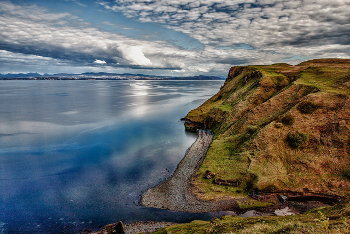
\includegraphics[width=\textwidth]{img/images/landscape.png}
                    \caption{Original Image.}
                \end{subfigure}
                \begin{subfigure}[b]{0.4\textwidth}
                    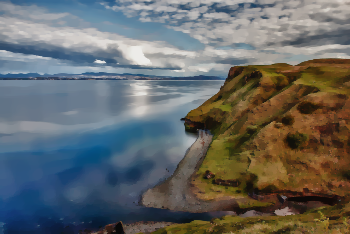
\includegraphics[width=\textwidth]{img/approximation/01landscape.png}
                    \caption{$\lambda = 0.1$.}
                \end{subfigure}
                \begin{subfigure}[b]{0.4\textwidth}
                    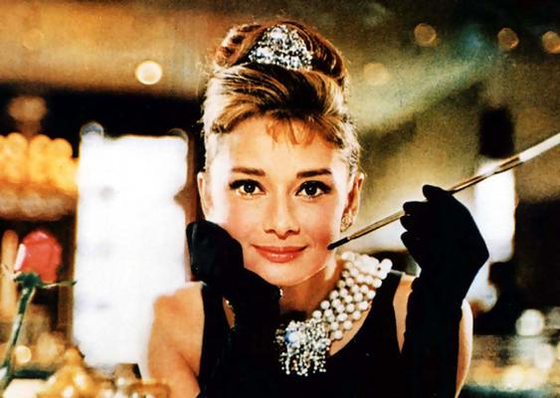
\includegraphics[width=\textwidth]{img/images/hepburn.png}
                    \caption{Original Image.}
                \end{subfigure}
                \begin{subfigure}[b]{0.4\textwidth}
                    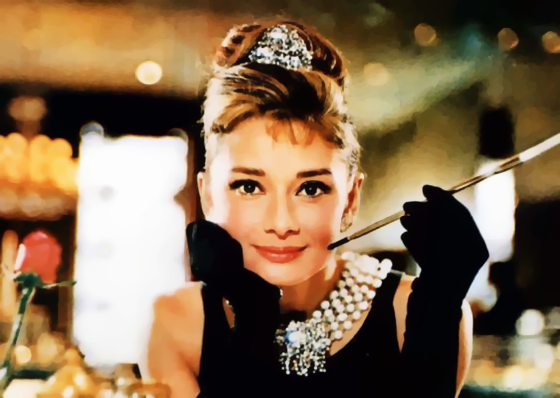
\includegraphics[width=\textwidth]{img/approximation/01hepburn.png}
                    \caption{$\lambda = 0.1$.}
                \end{subfigure}
                \caption[First estimate of $\lambda$ for the ROF model.]{Approximation of the Landscape and Audrey Hepburn image with the proposed $\lambda$.}
            \label{fig:estimation_of_lambda_rof}
            \end{figure}

        \subsection{Estimation of $\boldsymbol{\tau}$}
        \label{sub:estimation_of_tau_rof}

            We find that for $\lambda = 0.1$ the best choice for the time-step is $\tau = 0.73$. We observe this value by running tests for $\tau$ starting at $0.01$ and increasing it by $0.01$ until we reach $0.99$. For this test procedure we make use of three different images: Lena (grayscaled), Hepburn (RGB) and Landscape (RGB). The suggested $\tau$ leads to a acceptable number of iteration steps. This is also illustrated in Table \ref{tab:estimation_of_tau_rof}. But, as it turns out, the time-step parameter $\tau$ couples with the image $g$ and the parameter $\lambda$. Table \ref{tab:estimation_of_tau_rof} also reveals that the best estimates for $\tau$ vary a lot for each test image.
            \begin{table}[!ht]
                \centering
                \begin{tabular}{| l | l | l | l | l | l | l |}
                    \hline
                    & \multicolumn{2}{|c|}{Lena Image} & \multicolumn{2}{|c|}{Hepburn Image} & \multicolumn{2}{|c|}{Landscape Image} \\ \hline\hline
                    No. & $\tau$ & Iter & $\tau$ & Iter & $\tau$ & Iter \\ \hline
                    1 & 0.67 & 170 & 0.55 & 247 & 0.83 & 164 \\ \hline
                    2 & 0.68 & 170 & 0.56 & 247 & 0.84 & 164 \\ \hline
                    3 & 0.7 & 170 & 0.53 & 251 & 0.85 & 166 \\ \hline
                    4 & 0.73 & 170 & 0.57 & 251 & 0.79 & 167 \\ \hline
                    \vdots &  &  &  &  &  & \\ \hline
                    19 & 0.87 & 173 & 0.73 & 257 & 0.94 & 172 \\ \hline
                    \vdots &  &  &  &  &  & \\ \hline
                    22 & 0.61 & 174 & 0.63 & 260 & 0.73 & 174 \\ \hline
                \end{tabular}
                \caption[Best estimate of $\tau$ for the ROF model.]{Setting $\tau = 0.73$ provides a good guess for fast convergence.}
                \label{tab:estimation_of_tau_rof}
            \end{table}
            The coupling of $\lambda$ and $\tau$ can be seen, if we set $\tau = 0.73$ and $\lambda = 0.2$ and approximate for instance the Landscape image. We only increase $\lambda$ by a factor of $2$, but the number of iterations for this setting drop to $121$. If we decrease $\lambda$ by a factor of $2$, setting $\lambda = 0.05$, we obtain $288$ iteration steps. We earlier discussed that a higher value for $\lambda$ leads to an approximation $u$ which is closer to the input image $g$. Our test shows that the algorithm converges faster if the data fidelity term is weighted higher. Overall, we see that finding a $"$perfect$"$ time-step is not possible. So, we provide a good guess for which the algorithm is likely to converge fast.\\
            \begin{table}[!ht]
                \centering
                \begin{tabular}{| l || l | l | l |}
                    \hline
                    & Iterations & CPU time & GPU time \\ \hline
                    Lena & 170 & 1.13 s & 0.025 s \\ \hline
                    Hepburn & 257 & 4.13 s & 0.049 s \\ \hline
                    Landscape & 174 & 1.03 s & 0.032 s \\ \hline
                \end{tabular}
                \caption[Run-times for best parameters in ROF model.]{Setting $\tau = 0.73$ and $\lambda = 0.1$ yields good results and a fast run-time. The parallelized version is up to $84$ times faster than the serial version.}
                \label{tab:rof_cpu_vs_gpu}
            \end{table}

        To this end, we suggest the setting $\theta = 1$, $\lambda = 0.1$ and $\tau = 0.73$ for the primal-dual algorithm, for which we derive the approximation $u$ of $g$ in a reasonable run-time, see also Table \ref{tab:rof_cpu_vs_gpu}, and good results. In parallel we can achieve a performance increase up to a factor of $84$.

    \section{Image Approximation using the TVL1 Model} % (fold)
    \label{sec:image_approximation_using_the_tvl1_model}

        We now turn our focus on the TVL1 model. As we did for the ROF model we provide the examples and parameter estimations depending on our serial C++ code in this section. We additionally provide the run-times on the GPU. Fortunately, we can adapt a lot of operations from the previous section. The gradient operators and computation of the proximity operator for $F^{\ast}(p) = \delta_{P}(p)$ remain completely the same. The primal-dual algorithm with the extrapolation step is consistent and can be adapted. The only difference to the ROF model is the computation of $(\textnormal{Id} + \tau\,\partial\,G)^{-1}(\tilde{u})$. In Equation (\ref{eq:prox_g_tvl1}) we showed how proximity operator is computed. If we apply this computation to each color channel $k = 1, ..., B$ we add the index $k$ to our notation. This means that our update on the variable $u$, or more precisely $u^{n+1}_{i,j,k}$, depends on the current estimate $\tilde{u}$ and the input image $g$. To save run-time, we pre-compute $fac = \tau * \lambda \,\,\,\,\,\, \textnormal{and} \,\,\,\,\,\, est = u^{n}_{i,j,k} - g_{i,j,k}$. Since these values need to be computed in each if-statement, we calculate it once - before the if-statements occur - and make use of the values:
            $$
                u^{n+1}_{i,j,k} = 
                    \begin{dcases*}
                        u^{n}_{i,j,k} - fac & \textnormal{if\, $est > fac$} \\
                        u^{n}_{i,j,k} + fac & \textnormal{if\, $est < - fac$} \\
                        g_{i,j,k} & \textnormal{if\, $|est| \le fac$}
                    \end{dcases*}.
            $$
        Now, the only thing we need to change in the primal descent C++ function ($primal\_desc$) is the last line of code in the inner for-loops. In this line, we compute the proximity operator, so we fit the code to the TVL1 model and obtain the following C++ function:
        \begin{lstlisting}
template<typename T>
void primal_desc(T* p_x, T* p_y, T* u, T* g, T tau, T lambda, int M, int N, int B) {
  T dx, dy, sum, est;
  T fac = tau*lambda;
  int index;
  for (int k = 0; k < B; k++) {
    for (int i = 0; i < N; i++) {
      for (int j = 0; j < M; j++) {
        index = j + i * M + k * N * M;
        dx = (i+1<N ? p_x[index] : 0.f) -
             (i>0 ? p_x[j + (i-1) * M + k * N * M] : 0.f);
        dy = (j+1<M ? p_y[index] : 0.f) -
             (i>0 ? p_y[(j-1) + i * M + k * N * M] : 0.f);
        sum = u[index] + tau * (dx + dy);
        est = sum - g[index];
        if (est > fac) u[index] = sum - fac;
        if (est < -fac) u[index] = sum + fac;
        if (abs(est) <= fac) u[index] = g[index];
      }
    }
  }
}
        \end{lstlisting} 
        With these few substitutions the TVL1 model is already set up. It is now left to provide good estimates for the input values $\lambda$ and $\tau$. We set again $\theta = 1$ and allocate $u, \bar{u}, g \in [0, 255]^{B}$, where $B$ is the number of color channels.
        \subsection{Estimation of $\boldsymbol{\lambda}$} % (fold)
        \label{sub:estimation_of_lambda_tvl1}
            For the estimation of $\lambda$ we make the same assumptions as in Subsectoin \ref{sub:estimation_of_lambda_rof}. We choose
                $$
                    \lambda \in \{ 0.01, 0.02, 0.03, 0.04, 0.05, 0.06, 0.07, 0.08, 0.09, 0.1, 0.2, 0.3, 0.4, 0.5 \}
                $$
            and seek for a value $PSNR(g, u)$ in the range of $[30, 36]$. We see in Table \ref{tab:estimation_of_lambda_tvl1} that the parameter $\lambda$ again couples with the input image. As in the ROF model, the structure of an image plays an important role. If we compare the PSNR values of the Landscape to those of the Audrey Hepburn image for some settings of $\lambda$, we see tremendous variations. Additionally, also taking the PSNR of the grayscaled Lena image into account, these differences are even more extreme.
            \begin{table}[!ht]
                \centering
                \begin{tabular}{| l | l | l | l | l | l | l |}
                    \hline
                    & \multicolumn{2}{|c|}{Lena Image} & \multicolumn{2}{|c|}{Hepburn Image} & \multicolumn{2}{|c|}{Landscape Image} \\ \hline\hline
                    $\lambda$ & Iter & PSNR & Iter & PSNR & Iter & PSNR \\ \hline
                    0.7 & 281 & 32 & 541 & 29 & 653 & 24 \\ \hline
                    0.8 & 251 & 33 & 442 & 31 & 659 & 25 \\ \hline
                    0.9 & 246 & 34 & 415 & 32 & 621 & 25 \\ \hline
                    1.0 & 217 & 35 & 383 & 33 & 554 & 26 \\ \hline
                    1.1 & 208 & 36 & 330 & 34 & 527 & 26 \\ \hline
                    1.2 & 198 & 36 & 299 & 35 & 514 & 27 \\ \hline
                \end{tabular}
                \caption[Best estimate of $\lambda$ for the TVL1 model.]{Setting $\lambda = 0.7$ for grayscaled and $\lambda = 1.2$ for colored images provides a suitable framework.}
                \label{tab:estimation_of_lambda_tvl1}
            \end{table}
            For instance if we set $\lambda = 0.7$ we observe a PSNR of $32$ for the Lena image. But the Hepburn image only attains a value of $29$ and the Landscape image $24$. This means that the PSNR varies in a range of $8$ and for this finding a perfect fit is not possible. Overall, we suggest to set $\lambda = 0.7$ for grayscaled images and $\lambda = 1.2$ for color images. Relating to Table \ref{tab:estimation_of_lambda_tvl1} this setting seems to be accurate. Let us check if there exists a time-step $\tau$ for which the algorithm convergences quickly with the suggested values for $\lambda$.
        % subsection best_ (end)
        \subsection{Estimation of $\boldsymbol{\tau}$} % (fold)
        \label{sub:estimation_of_tau_tvl1}
            
            We apply the same procedure to estimate the best time-step parameter $\tau$ as in Subsection \ref{sub:estimation_of_tau_rof}. We use again the images Lena, Audrey Hepburn and Landscape for the evaluation. There are several parameters which appear under the quickest run-times. The one which is most likely to guarantee a fast convergence is $\tau = 0.98$, cf. Table \ref{tab:tvl1_cpu_vs_gpu}. In the parallel version we observe a tremendous run-time decrease up to a factor of $150$. Even if we used grayscaled and colored images with $\lambda = 0.7$ and $\lambda = 1.2$, respectively, this $\tau$ appears to be a good choice. Since we have a coupling of the image and the parameters $\lambda$ and $\tau$, as in the ROF model, this suggested $\tau$ is likely to obtain a fast convergence.
            \begin{table}[!ht]
                \centering
                \begin{tabular}{| l || l | l | l | l |}
                    \hline
                    & $\lambda$ & Iterations & CPU time & GPU time \\ \hline
                    Lena & 0.7 & 210 & 2.97 s & 0.034 s \\ \hline
                    Hepburn & 1.2 & 254 & 7.85 s & 0.052 s \\ \hline
                    Landscape & 1.2 & 210 & 3.69 s & 0.040 s \\ \hline
                \end{tabular}
                \caption[Run-times for best parameters in TVL1 model.]{Setting $\tau = 0.98$ results in a fast run-time. Parallelization yields a performance increase up to a factor $150$.}
                \label{tab:tvl1_cpu_vs_gpu}
            \end{table}
            In Figure \ref{fig:best_tvl1_landscape} (b) we show the result for our suggested framework by setting $\theta = 1, \lambda = 1.2$ and $\tau = 0.98$ using the Landscape image. Even though the TVL1 model yields good approximations, we clearly see that it is not able to preserve edges well enough if we choose $\lambda$ too small. For instance in (c) of the same figure we see that some contours vanish and we see over-smoothing in the image if we set $\lambda = 0.7$.\\
            \begin{figure}[!ht]
                \centering
                \begin{subfigure}[b]{0.32\textwidth}
                    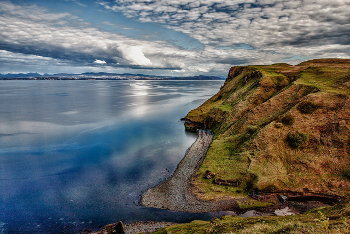
\includegraphics[width=\textwidth]{img/images/landscape.png}
                    \caption{The original Landscape image.}
                \end{subfigure}
                \begin{subfigure}[b]{0.32\textwidth}
                    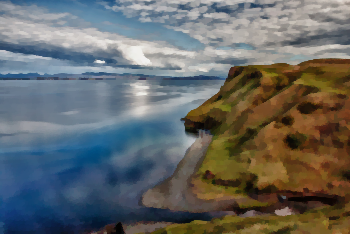
\includegraphics[width=\textwidth]{img/approximation/12landscape.png}
                    \caption{Approximation using $\lambda = 1.2$.}
                \end{subfigure}
                \begin{subfigure}[b]{0.32\textwidth}
                    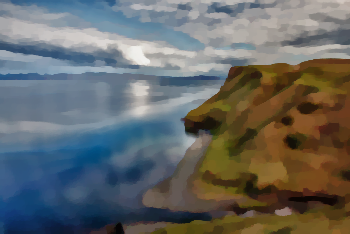
\includegraphics[width=\textwidth]{img/approximation/07landscape.png}
                    \caption{Approximation using $\lambda = 0.7$.}
                \end{subfigure}
                \caption[Best approximation using the TVL1 model with Landscape image.]{Approximation of the Landscape image with the TVL1 model.}
                \label{fig:best_tvl1_landscape}
            \end{figure}
            
            Overall, the TVL1 model yields good approximations $u$ and is able to remove Gaussian and salt and pepper noise from images. We will discuss this application in Section \ref{sec:image_denoising}.
        % subsection best_tau_estimation (end)
    % section image_approximation_using_the_tvl1_model (end)

    \section{Image Approximation using the Real-Time Minimizer} % (fold)
    \label{sec:image_approximation_using_the_real_time_minimizer}
        
        In the case of the real-time minimizer for the Mumford-Shah model, which only has real-time applicability on a GPU, we can adapt most of the code from the ROF model. Even though it runs in real-time, we are more interested in the framework itself. As before our estimation is done with the serial C++ implementation and we additionally provide the run-times of the GPU version. The function $G$ is almost the same as in the ROF model except the factor $\frac{\lambda}{2}$. So, we only exchange the line
            $$
                u[index] = (sum + tau * lambda * g[index]) / (1.f + tau * lambda)
            $$
        by
            $$
                u[index] = (sum + 2 * tau * g[index]) / (1.f + 2 * tau)
            $$
        in the primal descent function ($primal\_desc$). In the dual ascent C++ function ($dual\_asc$) we need to exchange two lines of code, where we take into account that the proximity operator for $R_{MS}^{\ast}(\tilde{p})$ is computed by
            $$
                p = \left( \textnormal{Id} + \sigma \partial R_{MS}^{\ast} \right)^{-1}(\tilde{p}) \iff p_{i,j} =
                    \begin{dcases*}
                        \frac{\lambda}{\lambda + \sigma} \tilde{p}, & \textnormal{if $|\tilde{p}| \le \sqrt{\frac{\nu}{\lambda}\sigma(\sigma + 2\lambda)}$} \\
                        0 & \textnormal{else}
                    \end{dcases*}.
            $$
        We pre-compute some values and use them afterwards in each calculation. Additionally, we add again the index $k$ with $k = 1, ..., B$ to each variable. We set
            \begin{eqnarray}
                fac = (2 * \lambda) / (\sigma + 2 * \lambda) \,\,\, \textnormal{and} \notag \\
                p\_abs = |p^{n}_{i,j,k}| = \sqrt{dx*dx+dy*dy} \notag
            \end{eqnarray}
        and compute the bound by $bnd = \sqrt{(\nu / \lambda) * \sigma * (\sigma + 2 * \lambda)}$. Then we rewrite the proximity operator to
            $$
                p^{n+1}_{i,j,k} =
                    \begin{dcases*}
                        fac*p^{n}_{i,j,k} & \textnormal{if $p\_abs \le bnd$} \\
                        0 & \textnormal{else}
                    \end{dcases*}.
            $$
        We change the computations, in which we compute $p^{n+1}_{x}$ and $p^{n+1}_{y}$ with respect to the proximity operator of $R_{MS}^{\ast}(\tilde{p}^{n})$, and observe the new version of the C++ function by:
        \begin{lstlisting}
template<typename T>
void dual_asc(T* p_x, T* p_y, T* u_bar, T sigma, T lambda, T nu, int M, int N, int B) {
  T dx, dy;
  int index;
  T fac = (2 * lambda) / (sigma + 2 * lambda);
  T B = sqrt((nu / lambda) * sigma * (sigma + 2 * lambda));
  for (int k = 0; k < B; k++) {
    for (int i = 0; i < N; i++) {
      for (int j = 0; j < M; j++) {
        index = j + i * M + k * N * M;
        dx = i+1<N ? u_bar[j + (i+1) * M + k * N * M]-u_bar[index] : 0;
        dy = j+1<M ? u_bar[(j+1) + i * M + k * N * M]-u_bar[index] : 0;
        dx = p_x[index] + sigma * dx;
        dy = p_y[index] + sigma * dy;
        p_abs = sqrt(dx*dx+dy*dy);
        p_x[index] = p_abs <= bnd ? fac * dx : 0;
        p_y[index] = p_abs <= bnd ? fac * dy : 0;
      }
    }
  }
}
        \end{lstlisting}
        Using the proposed stopping criterion of Subsection \ref{sub:the_proximity_operators_of_the_mumford_shah_model}, we compute after each iteration step of the primal-dual algorithm
            $$
                ||u^{n+1} - u^{n}|| \le \varepsilon,
            $$
        with $\varepsilon = 5 \cdot 10^{-5}$. Strekalovskiy and Cremers suggest in \cite{Strekalovskiy-Cremers-eccv14} the same setting but evaluate the norm only once every ten iterations. As we used the second primal-dual algorithm of Section \ref{sec:a_firs_order_primal_dual_algorithm}, namely Algorithm \ref{alg:realtime_primal_dual_algorithm}, we additionally propose this version in C++ code:
        \begin{lstlisting}
template<typename T>
void RealTimeMinimizer(T* u, T* g, T lambda, T nu, int M, int N, int B, int iter) {
  T tau = 1.f / 4.f;
  T sigma = 1.f / 2.f;
  T theta = 2.f;
  T eps = 5*1E-5;
  T* u_bar = new T[M*N*B];
  T* u_prev = new T[M*N*B];
  T* p_x = new T[M*N*B];
  T* p_y = new T[M*N*B];

  for (int k = 1; k <= iter; k++) {
    dual_asc(p_x, p_y, u_bar, sigma, lambda, nu, M, N, B);
    primal_desc(p_x, p_y, u, g, tau, M, N, B);
    theta = (T)1 / sqrt(1 + 4 * tau); tau *= theta; sigma /= theta;
    extrapolation(u_bar, u, u_prev, theta, M, N, B);
    if (k%10 == 0) {
      if (Stop(u, u_n, M, N, B) <= eps) {
        break;
      }
    }
  }

  delete [] u_bar;
  delete [] u_prev;
  delete [] p_x;
  delete [] p_y;
}
        \end{lstlisting}
        The difference in this framework is that the primal-dual function does not take the parameter $\tau$ as an argument, because Algorithm \ref{alg:realtime_primal_dual_algorithm} suggests that this value is fixed by initialization. Instead the function takes the second parameter of the corresponding model, namely $\nu$. Additionally, we compute the updates on $\theta, \tau$ and $\sigma$ in each iteration step of the primal-dual algorithm. For this particular framework we followed Strekalovskiy and Cremers in \cite{Strekalovskiy-Cremers-eccv14} and use that $u, \bar{u}, g \in [0,1]^{B}$, where $B$ is the number of color channels.

        \subsection{Estimation of $\boldsymbol{\lambda}$ and $\boldsymbol{\nu}$} % (fold)
        \label{sub:estimation_of_lambda_and_nu_rt}
            
            For this model we have two parameters which can be combined in a lot of ways. We set $\lambda \in \{2, 20, 500\}$ to determine if $2$ or $20$ fits better in the piecewise-smooth case and use $500$ to evaluate the piecewise-constant case. Then, we need to find a suitable parameter $\nu$ for the different $\lambda$. So, we test each $\lambda$ with the setting for $\nu$ being an element of
                $$
                    \{0.01, 0.02, 0.03, 0.04, 0.05, 0.06, 0.07, 0.08, 0.09, 0.1, 0.2, 0.3, 0.4, 0.5, 0.6, 0.7, 0.8, 0.9, 1.0 \}.
                $$
            \begin{figure}[!ht]
                \centering
                \begin{subfigure}[b]{0.4\textwidth}
                    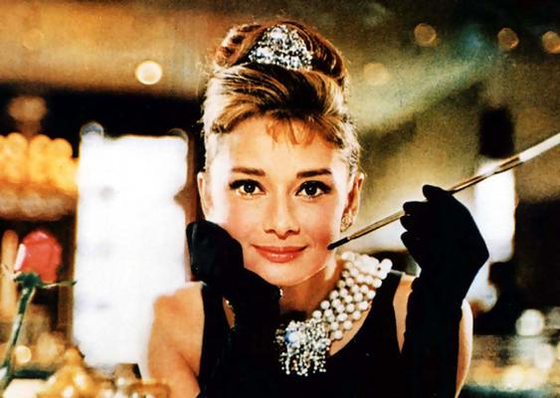
\includegraphics[width=\textwidth]{img/images/hepburn.png}
                    \caption{Original image.}
                \end{subfigure}
                \begin{subfigure}[b]{0.4\textwidth}
                    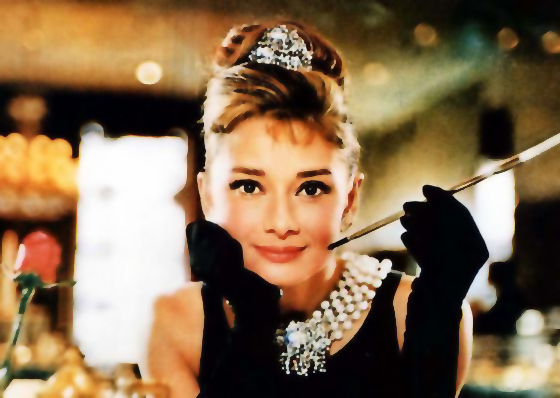
\includegraphics[width=\textwidth]{img/cartooning/bad_pws_hepburn.png}
                    \caption{$\lambda = 2, \nu = 0.1$.}
                \end{subfigure}
                \begin{subfigure}[b]{0.4\textwidth}
                    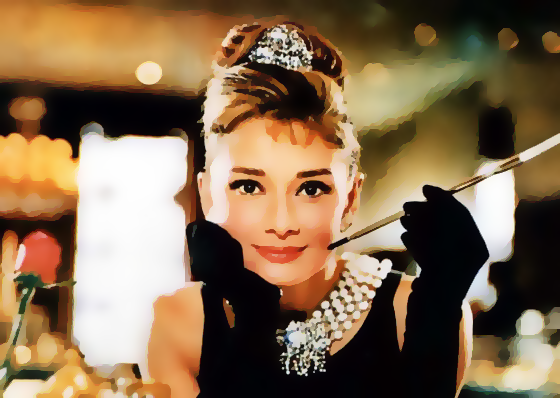
\includegraphics[width=\textwidth]{img/cartooning/best_pws_hepburn.png}
                    \caption{$\lambda = 20, \nu = 0.03$}
                \end{subfigure}
                \begin{subfigure}[b]{0.4\textwidth}
                    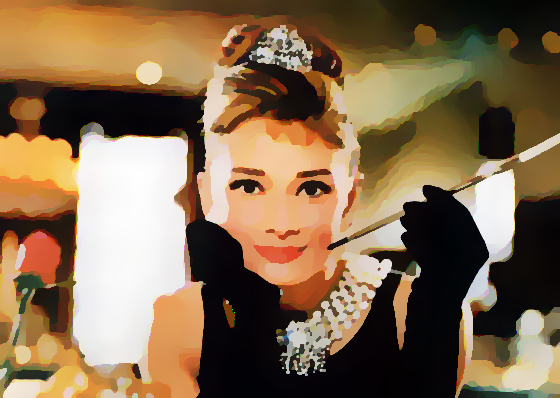
\includegraphics[width=\textwidth]{img/cartooning/best_pwc_hepburn.png}
                    \caption{$\lambda = 500, \nu = 0.1$}
                \end{subfigure}
                \caption[Comparing Audrey Hepburn pwc. and pws. using real-time Mumford-Shah model.]{Approximation of the Audrey Hepburn image with the piecewise-smooth (c) and piecewise-constant (d) Mumford-Shah model. In (b) one can see that $\lambda = 2$ is too weak and can cause blurring of the image.}
            \label{fig:estimation_of_lambda_and_nu_rt}
            \end{figure}
            We use again the images of Lena and Audrey Hepburn and the Landscape image and seek for a $PSNR(g, u)$ in the range $[30, 36]$ in the piecewise-smooth case. In the piecewise-constant case, which we consider first, we choose settings with a PSNR in the range $[20, 25]$. It turns out that several settings occur, which can be chosen in the piecewise-constant model. As possible $\nu$ all outcomes vary around $\nu = 0.1$, which we suggest to use. For the piecewise-smooth model we observe a lot of different estimations and the PSNR for each image provides different suggestions. Since this procedure is more a guessing than an evaluation, we compare the approximations $u$ in terms of the approximations. We find that $\lambda = 2$ is too weak. These approximations are noisy and sometimes blurred. For this we conclude that a suitable setting for $\lambda$ in the piecewise-smooth case is $\lambda = 20$. If we then choose $\nu = 0.03$, we observe PSNR values $31$ (Lena), $25$ (Landscape) and $30$ (Audrey Hepburn). In terms of the Audrey Hepburn image, Figure \ref{fig:estimation_of_lambda_and_nu_rt} shows the outcomes for our suggested settings. Further, it reveals that $\lambda = 2$ is indeed not a suitable choice.\\
            \begin{table}[!ht]
                \parbox{.9\linewidth}{
                \centering
                    \begin{tabular}{| l || l | l | l | l | l |}
                        \hline
                         & $\lambda$ & $\nu$ & Iterations & CPU time & GPU time \\ \hline
                        Lena        & 20  & 0.03 & 21 & 0.085 s & 0.004 s \\ \hline
                        Lena        & 500 & 0.1  & 12 & 0.050 s & 0.002 s \\ \hline
                        Hepburn     & 20  & 0.03 & 40 & 0.360 s & 0.008 s \\ \hline
                        Hepburn     & 500 & 0.1  & 66 & 0.620 s & 0.013 s \\ \hline
                        Landscape   & 20  & 0.03 & 44 & 0.150 s & 0.008 s \\ \hline
                        Landscape   & 500 & 0.1  & 54 & 0.190 s & 0.010 s \\ \hline
                    \end{tabular}
                }
                \caption[Run-Times for best parameters real-time framework.]{Estimated run-times on a CPU and GPU for our three test images. The parallel version is up to $47$ times faster than the CPU version.}
                \label{tab:realtime_cpu_vs_gpu}
            \end{table}
            
        In Table \ref{tab:realtime_cpu_vs_gpu} we find the run-times for our suggested setting. With a performance increase up to a factor of $47$ the parallel version has indeed a real-time applicability. In this model there is no need to find a good estimate of the time-step $\tau$, because this value is updated in each iteration seperately and is coupled with the parameter $\theta$. As suggested in Algorithm \ref{alg:realtime_primal_dual_algorithm} we pre-compute it with $\tau = \frac{1}{2d}$, where $d = 2$, since the dimension of $\Omega$ is two. Let us now turn our focus on applications to imaging. We start with one application of the real-time minimizer of the Mumford-Shah functional, namely image cartooning.

        % subsection estimation_of_lambda_and_nu_rt (end)

    % section approximation_using_the_real_time_minimizer (end)

    \section{Image Cartooning} % (fold)
    \label{sec:image_cartooning}
        
        In this section we present a technique to turn an input image $g$ into a cartooned image $u$. For this we will make use of the real-time minimizer for the Mumford-Shah functional. We further introduce a concept to highlight the edges in the cartooned images, first proposed in \cite{Strekalovskiy-Cremers-eccv14}. For this we make explicit use of the set $K_{MS}$, as modeled in Equation (\ref{eq:edge_set_k}). We then present cartooned images - piecewise-constant approximations - with edge highlighting.

        % subsection another_data_fidelity_term (end)

        \subsection{Edge Highlighting} % (fold)
        \label{sub:edge_highlighting}
            
            \begin{figure}[!ht]
                \centering
                \begin{subfigure}[b]{0.32\textwidth}
                    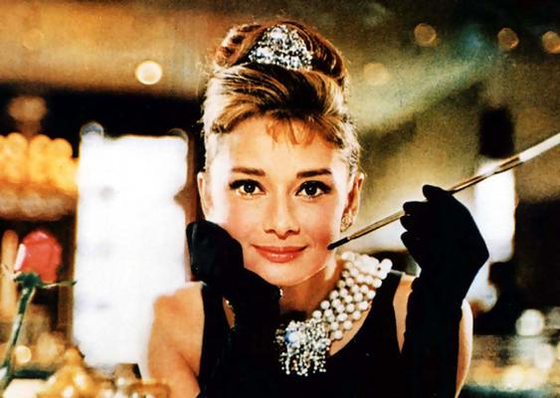
\includegraphics[width=\textwidth]{img/images/hepburn.png}
                    \caption{Original image.}
                \end{subfigure}
                \begin{subfigure}[b]{0.32\textwidth}
                    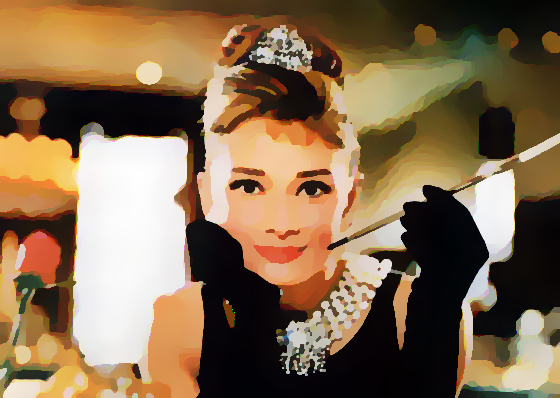
\includegraphics[width=\textwidth]{img/cartooning/best_pwc_hepburn.png}
                    \caption{Without edge highlighting.}
                \end{subfigure}
                \begin{subfigure}[b]{0.32\textwidth}
                    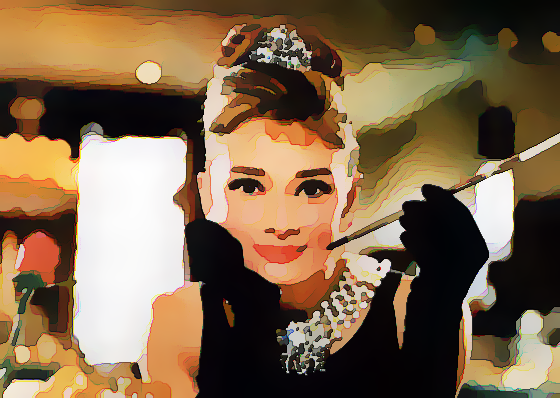
\includegraphics[width=\textwidth]{img/cartooning/best_pwc_hepburn_eh.png}
                    \caption{With edge highlighting.}
                \end{subfigure}
                \begin{subfigure}[b]{0.32\textwidth}
                    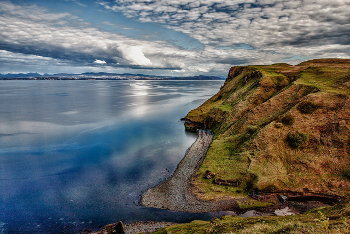
\includegraphics[width=\textwidth]{img/images/landscape.png}
                    \caption{Original image.}
                \end{subfigure}
                \begin{subfigure}[b]{0.32\textwidth}
                    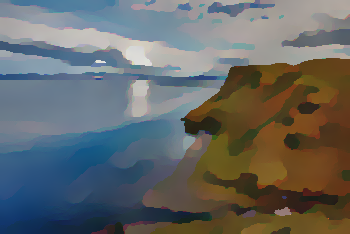
\includegraphics[width=\textwidth]{img/cartooning/best_pwc_landscape.png}
                    \caption{Without edge highlighting.}
                \end{subfigure}
                \begin{subfigure}[b]{0.32\textwidth}
                    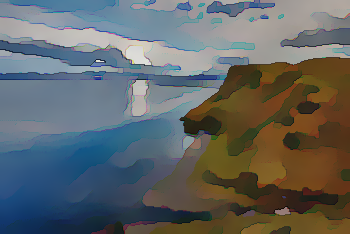
\includegraphics[width=\textwidth]{img/cartooning/best_pwc_landscape_eh.png}
                    \caption{With edge highlighting.}
                \end{subfigure}
                \caption[Cartooning example of Audrey Hepburn and Landscape image.]{Cartooning of the Audrey Hepburn and Landscape image with $\lambda = 500$ and $\nu = 0.1$.}
            \label{fig:cartooning_hepburn_and_landscaperealtime}
            \end{figure}
            The idea, proposed by Strekalovskiy and Cremers in \cite{Strekalovskiy-Cremers-eccv14}, is to use the edge set $K_{MS}$ in order to highlight edges in the approximation $u$. For that assume $(i,j) \in K_{MS}$, then we have $|(\nabla u)_{i,j}| \ge \sqrt{\frac{\nu}{\lambda}}$ by definition of $K_{MS}$. This notation is equivalent to
                \begin{equation}
                    \frac{|(\nabla u)_{i,j}|}{\sqrt{\frac{\nu}{\lambda}}} \ge 1.
                    \label{eq:first_inequality}
                \end{equation}
            Further, we compute $|(\nabla u)_{i,j}| \le \sqrt{2}$. This equation holds with the definition for $\nabla$, cf. Definition \ref{def:discrete_gradient_operator}, and having $u_{i,j} \in [0, 1]$ for all $i = 1, ..., N$ and $j = 1, ..., M$. Then
                \begin{eqnarray}
                    |(\nabla u)_{i,j}| &=& \sqrt{\underbrace{(u_{i+1,j} - u_{i,j})^{2}}_{\le 1} + \underbrace{(u_{i,j+1} - u_{i,j})^{2}}_{\le 1}} \notag \\
                    &\le& \sqrt{1 + 1} \notag \\
                    &=& \sqrt{2} \notag
                \end{eqnarray}
            Together with Equation \ref{eq:first_inequality} it follows
                $$
                    1 \le \frac{|(\nabla u)_{i,j}|}{\sqrt{\frac{\nu}{\lambda}}} \le \frac{\sqrt{2}}{\sqrt{\frac{\nu}{\lambda}}}.
                $$
            Applying the logarithm function, which is monotonically increasing, to each of the terms we get
                $$
                    0 \le \log \left( \frac{|(\nabla u)_{i,j}|}{\sqrt{\frac{\nu}{\lambda}}} \right) \le \log \left( \frac{\sqrt{2}}{\sqrt{\frac{\nu}{\lambda}}} \right).
                $$
            If we now divide each term by the one on the rightmost, we observe
                $$
                    0 \le \frac{\log \left( \frac{|(\nabla u)_{i,j}|}{\sqrt{\frac{\nu}{\lambda}}} \right)}{\log \left( \frac{\sqrt{2}}{\sqrt{\frac{\nu}{\lambda}}} \right)} \le 1.
                $$
            With these calculations, we now define a $v \in [0, 1]$ by
                $$
                    v := \frac{\log \left( \frac{|(\nabla u)_{i,j}|}{\sqrt{\frac{\nu}{\lambda}}} \right)}{\log \left( \frac{\sqrt{2}}{\sqrt{\frac{\nu}{\lambda}}} \right)}.
                $$
            Then, the parameter $v$ only increases if $|(\nabla u)_{i,j}|$ increases and decreases if $|(\nabla u)_{i,j}|$ decreases, because $\sqrt{\frac{\nu}{\lambda}}$ is a constant factor and the logarithm function is monotonically increasing. The value $v$ serves as an edge indicator. The idea is to multiply each pixel value $u$ with
                $$
                    1 - v \in [0, 1],
                $$
            if $(i, j) \in K_{MS}$. On the other hand, if $(i, j) \notin K_{MS}$ the value $u$ is supposed to remain unchanged. Then points in the image domain $\Omega$ with strong edges are painted darker. Using the proposed values $\lambda = 500$ and $\nu = 0.1$, as suggested in Section \ref{sub:estimation_of_lambda_and_nu_rt}, we compare an approximation with and without edge highlighting. Figure \ref{fig:cartooning_hepburn_and_landscaperealtime} shows that this technique clearly yields darker edges. Since this highlighting takes place after the primal-dual algorithm, it does not slow down the code significantly.\\

        We implement this technique of edge highlighting in our framework and test it against the pure piecewise-constant approximation. Summarizing this method in a C++-function, we get:
            \begin{lstlisting}
template<typename T>
void edging(T* u, T lambda, T nu, int M, int N, int B) {
  for (int k = 0; k < B; k++) {
    for (int i = 0; i < N; i++) {
      for (int j = 0; j < M; j++) {
        int X = j + i * M + k * N * M;
        T dx = i + 1 < N ? u[j + (i+1) * M + k * N * M] - u[X] : 0;
        T dy = j + 1 < M ? u[j + 1 + i * M + k * N * M] - u[X] : 0;
        T norm = sqrt(dx*dx+dy*dy);
        T factor = sqrt(nu/lambda);
        if (norm >= factor) {
          T c = (T)1 / log(sqrt(2)/factor);
          u[X] = (1 - c * log(norm / factor)) * u[X];
        }
      }
    }
  }
}
            \end{lstlisting}
        % subsection edge_highlighting (end)
        
        In this section we showed that the Mumford-Shah real-time minimizer is good in cartooning images and has the advantage of the discrete modeled set $K_{MS}$, which can be used for edge highlighting. However, the real-time framework has another application, namely denoising. We present this case together with the ROF and TVL1 model, respectively, in the next section.
    % section image_cartooning (end)

    \section{Image Denoising} % (fold)
    \label{sec:image_denoising}
        
        The goal in image denoising is to remove noise from an input image $g$ and get a smooth approximation $u$. We find different kinds of noise on images. The two most common are Gaussian and salt and pepper noise. Where Gaussian noise is relatively easy to remove, salt and pepper noise is more robust, since it resembles extrem values white and black on images. The ROF model and real-time minimizer for the Mumford-Shah model can handle Gaussian noise quite well, but are not able to remove salt and pepper noise accurately. However, the TVL1 model is able to manage both. We evaluate parameters $\lambda$, $\nu$ and $\tau$ for all models concerning the image denoising process. In this evaluation we follow the same procedure as in the previous sections. In this section we provide the best choices for the parameters. All estimations can be found online at \cite{Bauer}.
        \subsection{Gaussian Noise} % (fold)
        \label{sub:gaussian_noise}
            In the case of the ROF model we find another parameter as in Subsection \ref{sub:estimation_of_lambda_rof}. Setting $\lambda = 0.03$ yields good results and we observe a $PSNR(u, g)$ of $29$, where $u$ is the approximation and $g$ corresponds to the original Lena image. For the real-time Mumford-Shah framework we find a lot of possible pairs $(\lambda, \nu)$. For this reason, we choose the pair which results in the visibly best results. So, we suggest to set $\lambda = 20$ and $\nu = 0.06$. At last we adapt the value $\lambda = 0.7$ for the TVL1 model from Subsection \ref{sub:estimation_of_lambda_tvl1}. We find that this value is a good fit to remove Gaussian noise with the TVL1 model. The approximations produced by the suggested values for $\lambda$ can be seen in Figure \ref{fig:denoising_lena_gauss}. All three models remove Gaussian noise quite accurate. Whereas the real-time model for the Mumford-Shah functional does not need an estimation for $\tau$, because this value is fixed, we further provide a suitable $\tau$ for the ROF and TVL1 model, respectively. In our tests we find that $\tau = 0.99$ with $359$ is the best estimate for removing Gaussian noise with the ROF model. Additionally, we find in Table \ref{tab:estimation_of_tau_denoising} some estimates for $\tau$ for the TVL1 model. If we set $\tau = 0.97$ we have a fast convergence for both: Removing Gaussian and salt and pepper noise. Because of this, we suggest this $\tau$ as our best fit for this model.
            \begin{figure}[!ht]
                \centering
                \begin{subfigure}[b]{0.244\textwidth}
                    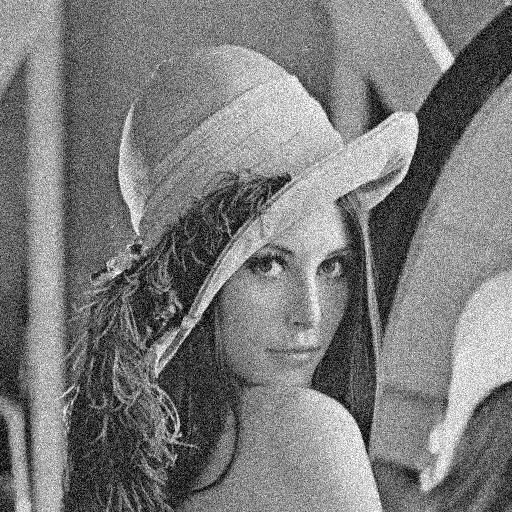
\includegraphics[width=\textwidth]{img/images/lena_gauss_noise.png}
                    \caption{Noisy image.\newline}
                \end{subfigure}
                \begin{subfigure}[b]{0.244\textwidth}
                    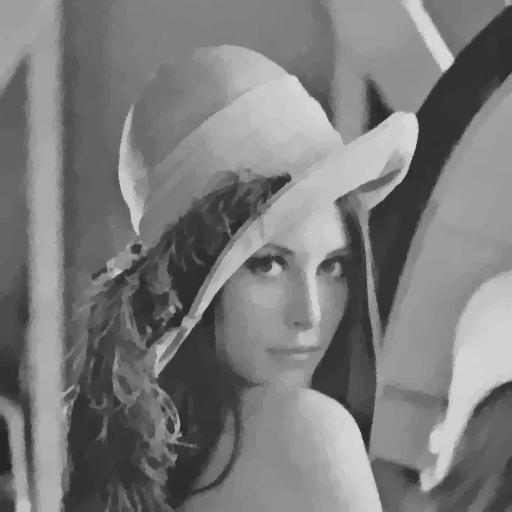
\includegraphics[width=\textwidth]{img/denoising/gauss_noise/003lena.png}
                    \caption{ROF: $\lambda = 0.03$.\newline}
                \end{subfigure}
                \begin{subfigure}[b]{0.244\textwidth}
                    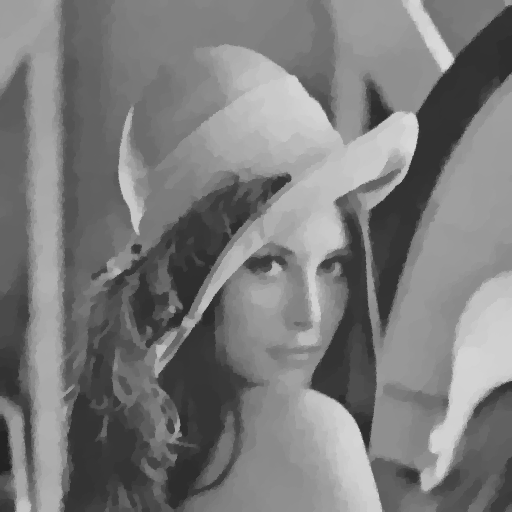
\includegraphics[width=\textwidth]{img/denoising/gauss_noise/07lena.png}
                    \caption{TVL1: $\lambda = 0.7$.\newline}
                \end{subfigure}
                \begin{subfigure}[b]{0.244\textwidth}
                    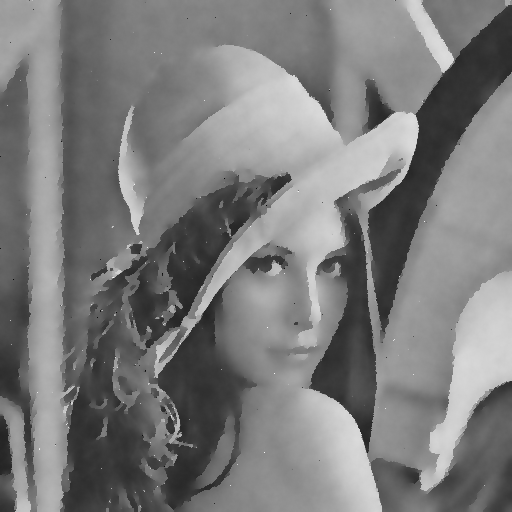
\includegraphics[width=\textwidth]{img/denoising/gauss_noise/2006.png}
                    \caption{MS: $\lambda = 20$\newline$\nu = 0.06$.}
                \end{subfigure}
                \caption[Removing Gaussian noise using the ROF, TVL1 and real-time Mumford-Shah framework.]{Removing Gaussian noise from the Lena image with the ROF, TVL1 and real-time Mumford-Shah framework.}
            \label{fig:denoising_lena_gauss}
            \end{figure}
        % subsection gaussian_noise (end)
        \subsection{Salt and Pepper Noise} % (fold)
        \label{sub:salt_and_pepper_noise}
            \begin{figure}[!ht]
                \centering
                \begin{subfigure}[b]{0.24\textwidth}
                    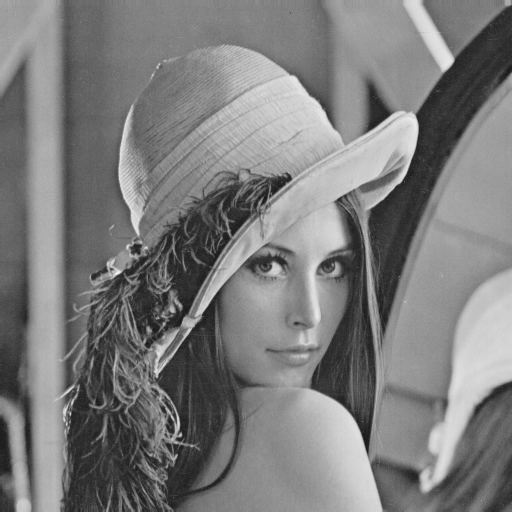
\includegraphics[width=\textwidth]{img/images/lena.png}
                    \caption{Original image.}
                \end{subfigure}
                \begin{subfigure}[b]{0.24\textwidth}
                    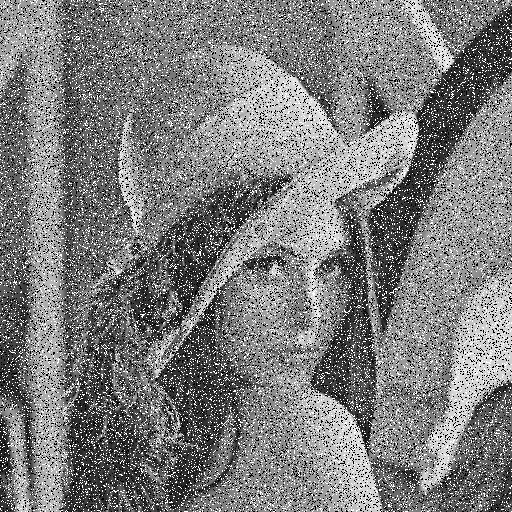
\includegraphics[width=\textwidth]{img/images/lena_sp_noise.png}
                    \caption{25\% noise.}
                \end{subfigure}
                \begin{subfigure}[b]{0.24\textwidth}
                    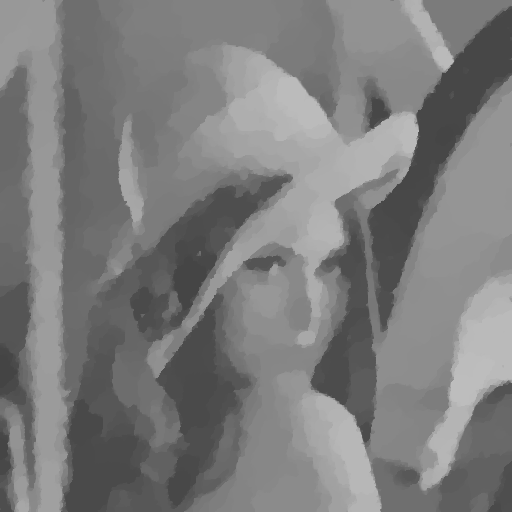
\includegraphics[width=\textwidth]{img/denoising/salt_and_pepper_noise/001lena.png}
                    \caption{$\lambda = 0.01$}
                \end{subfigure}
                \begin{subfigure}[b]{0.24\textwidth}
                    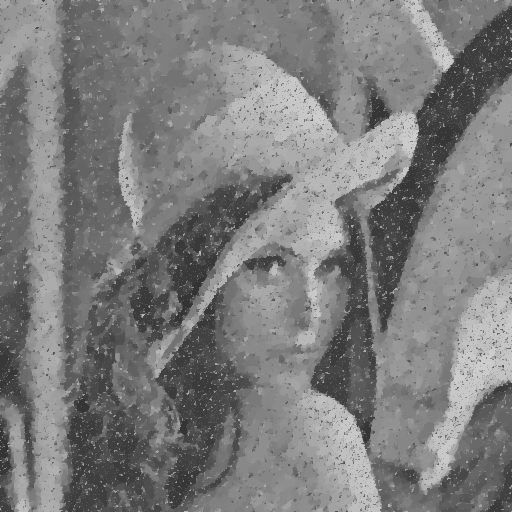
\includegraphics[width=\textwidth]{img/denoising/salt_and_pepper_noise/002lena.png}
                    \caption{$\lambda = 0.02$}
                \end{subfigure}
                \caption[Salt and pepper denoising example: ROF.]{Salt and pepper denoising of the Lena image with the ROF Model.}
            \label{fig:denoising_lena_rof_sap}
            \end{figure}
            \begin{table}[!ht]
                \centering
                \begin{tabular}{| l | l | l | l | l | l | l | l |}
                    \hline
                    \multicolumn{4}{|c|}{Gaussian Noise} & \multicolumn{4}{|c|}{Salt \& Pepper Noise} \\ \hline\hline
                    $\tau$ & Iter & CPU time & GPU time & $\tau$ & Iter & CPU time & GPU time \\ \hline
                    0.97 & 435 & 15.00 s & 0.176 s & 0.98 & 337 & 3.96 s & 0.054 s \\ \hline
                    0.96 & 436 & 14.90 s & 0.177 s & 0.97 & 339 & 3.99 s & 0.054 s \\ \hline
                    0.95 & 437 & 14.98 s & 0.177 s & 0.96 & 341 & 4.00 s & 0.054 s \\ \hline
                    0.94 & 438 & 15.05 s & 0.178 s & 0.95 & 344 & 4.05 s & 0.054 s \\ \hline
                \end{tabular}
                \caption[Best estimate of $\tau$ for the TVL1 model for denoising.]{Setting $\tau = 0.97$ leads to fast convergence in both cases using the TVL1 model.}
                \label{tab:estimation_of_tau_denoising}
            \end{table}
            The first thing we try to evaluate: Finding a parameter $\lambda$ for the ROF model, so that it can remove salt and pepper noise. In fact, we find a value, namely $0.01$, see also Figure \ref{fig:denoising_lena_rof_sap}. Even though the result is far away from perfect, the ROF model is able to remove this kind of noise in some sense. If we seek for a $\tau$ in the case of denoising images degraded with salt and pepper noise, we find $\tau = 0.99$ with $724$ iterations as the best fit. So, we suggest setting $\tau = 0.99$ for the ROF model. Furthermore, we are not able to find a pair $(\lambda, \nu)$ for the real-time minimizer of the Mumford-Shah model, which is able to remove salt and pepper noise. However, the TVL1 model, as mentioned, also handles salt and pepper noise. Figure \ref{fig:denoising_lena_tvl1_sap} shows the denoising of salt and pepper noise with $\lambda = 0.7$. If we test for a parameter $\tau$ to obtain fast convergence we find that $\tau = 0.97$ is the best choice, see also Table \ref{tab:estimation_of_tau_denoising}. Here, we see that this value for $\tau$ occurs under the four best estimates.\\
            \begin{figure}[!ht]
                \centering
                \begin{subfigure}[b]{0.31\textwidth}
                    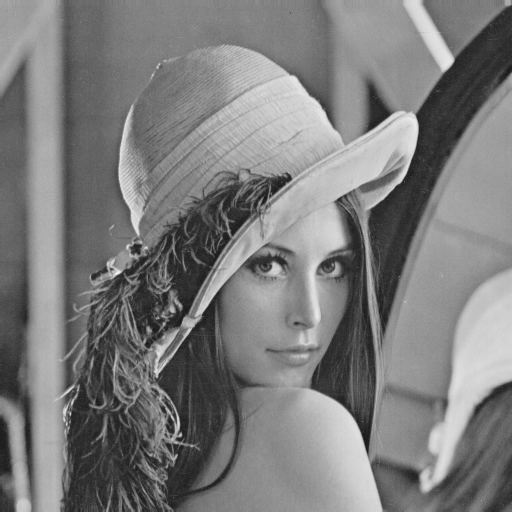
\includegraphics[width=\textwidth]{img/images/lena.png}
                    \caption{Original Image.}
                \end{subfigure}
                \begin{subfigure}[b]{0.31\textwidth}
                    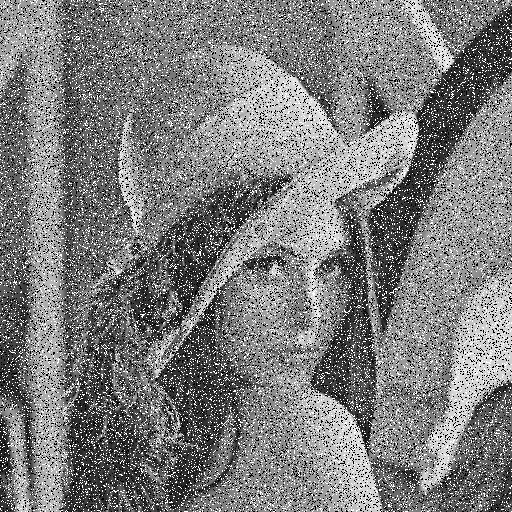
\includegraphics[width=\textwidth]{img/images/lena_sp_noise.png}
                    \caption{25\% Noise.}
                \end{subfigure}
                \begin{subfigure}[b]{0.31\textwidth}
                    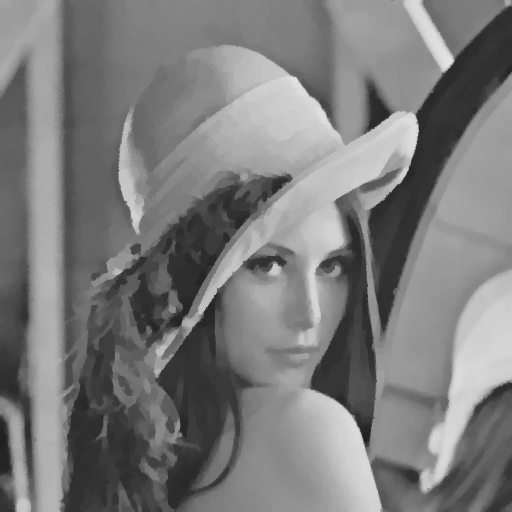
\includegraphics[width=\textwidth]{img/denoising/salt_and_pepper_noise/07lena.png}
                    \caption{$\lambda = 0.7$}
                \end{subfigure}
                \caption[Salt and pepper denoising example: TVL1.]{Salt and pepper denoising of the Lena image with the TVL1 Model.}
            \label{fig:denoising_lena_tvl1_sap}
            \end{figure}
        % subsection salt_and_pepper_noise (end)

        In the last section we will compare these three approaches against the convex relaxed Mumford-Shah functional for image denoising. We will see that the Mumford-Shah functional is indeed the best choice for removing Gaussian noise, because this model is edge preserving. Further, note that denoising color valued images is also straightforward. We can apply the proposed methods channel-wise and then derive denoised approximations of, for instance, RGB images.

    % section image_denoising (end)

    \section{Image Inpainting} % (fold)
    \label{sec:image_inpainting}

        Image inpainting is the process to restore or fill lost image data. Images which have a (huge) data loss can be inpainted by using a model based on the ROF energy. In this section we consider a modified version of the ROF model to derive a model for image inpainting. Let
            $$
                \mathcal{D} = \left\{ (i, j) \, | \, 1 \le i \le N, 1 \le j \le M \right\}
            $$
        denote the set of all discrete locations in our image domain. Since we know that data is missing in the underlying image, we additionally define a set $\mathcal{I} \subseteq \mathcal{D}$. This set holds all indices for which we have a data loss. The key idea is to take these two sets into account in the data fidelity term. We still use the total variaton as a regularizer, because we want to penalize jumps in the approximation $u$. But we approximate $u$ only in terms of existing data. We have
            \begin{equation}
                \min_{u \in X} \left( ||\nabla u||_{1} + \frac{\lambda}{2} \sum_{(i,j) \in \mathcal{D} \setminus \mathcal{I}} (u_{i,j} - g_{i,j})^{2} \right).
                \label{eq:inpainting_model}
            \end{equation}
        \begin{remark}
            According to Pock and Chambolle in \cite{Chambolle10afirst-order} we have two choices for $\lambda$:
                \begin{enumerate}
                    \item If we set $\lambda \in (0, \infty)$, the approximation $u$ is inpainted and denoised. This means the data fidelity term not only assures to keep the original data into account, but also removes noise in regions without data loss.
                    \item Setting $\lambda = \infty$ only yields to the inpainting case. So, if we have noisy regions, where no data loss appears, we get no smoothing and noise removement in these areas.
                \end{enumerate}
        \end{remark}
        Using the Legendre-Fenchel conjugate to rewrite this minimization problem into a saddle-point problem remains the same as in Section \ref{sec:the_rof_model}, since we set $F(\nabla u) = ||\nabla u||_{1}$ and $G(u) = \frac{\lambda}{2} \sum_{(i,j) \in \mathcal{D} \setminus \mathcal{I}} (u_{i,j} - g_{i,j})^{2}$. We obtain
            \begin{equation}
                \min_{u \in X} \max_{p \in Y} \left( \langle \nabla u, p \rangle  - \delta_{P}(p) + \frac{\lambda}{2} \sum_{(i,j) \in \mathcal{D} \setminus \mathcal{I}} (u_{i,j} - g_{i,j})^{2} \right),
                \label{eq:inpainting_primal_dual}
            \end{equation}
        where $P$ is as in Equation (\ref{eq:the_set_P}). Then we can identify $F^{\ast}(p) = \delta_{P}(p)$. But this also implies that the corresponding proximity operator for $F^{\ast}$ remains the same and we get:
            \begin{equation}
                p = (\textnormal{Id} + \sigma\,\partial\,F^{\ast})^{-1}(\tilde{p}) = \Pi_{P}(\tilde{p}) \iff p_{i,j} = \frac{\tilde{p}_{i, j}}{\max(1, |\tilde{p}_{i, j}|)},
            \label{eq:proximity_operator_f_star_inpainting}
            \end{equation}
        for all $i = 1, ..., N$ and $j = 1, ..., M$. If we want to apply our primal-dual algorithm to this model, we further need the proximity operator of the function $G$. In regions $\mathcal{D} \setminus \mathcal{I}$ this operator is the same as in the ROF model, since we have no changes in the data term. But we also need to take the regions $\mathcal{I}$ into account. As we set $G(u) = 0$ at each $(i,j) \in \mathcal{I}$, we compute the proximity operator by
            $$
                (\textnormal{Id} + \tau \partial G)^{-1}(\tilde{u}) = \arg \min_{u \in \mathcal{I}} \frac{||u - \tilde{u}||_{2}^{2}}{2}.
            $$
        Assume that $\hat{u} \in \arg \min_{u \in \mathcal{I}} \frac{||u - \tilde{u}||_{2}^{2}}{2}$, then with Proposition \ref{prop:zero_element_of_subgradient} we have
            $$
                0 \in \partial \left( \frac{||u - \tilde{u}||_{2}^{2}}{2} \right) \iff u = \tilde{u}.
            $$
        \begin{figure}[!ht]
            \centering
            \begin{subfigure}[b]{0.30\textwidth}
                \includegraphics[width=\textwidth]{img/images/lena.png}
                \caption{Original image.}
            \end{subfigure}
            \begin{subfigure}[b]{0.30\textwidth}
                \includegraphics[width=\textwidth]{img/images/lena_inpaint.png}
                \caption{Input image $g$.}
            \end{subfigure}
            \begin{subfigure}[b]{0.30\textwidth}
                \includegraphics[width=\textwidth]{img/inpainting/01lena.png}
                \caption{$\lambda = 0.1, \tau = 0.97$}
            \end{subfigure}
            \caption[Inpainting with seventy percent data loss with denoising.]{Inpainting of the Lena image with a data loss of seventy percent and simultanously denoising.}
        \label{fig:inpainting_lena_rof}
        \end{figure}
        Overall, we have pointwise for all $i = 1, ..., N$ and $j = 1, ..., M$
            \begin{equation}
                u = (\textnormal{Id} + \tau \partial G)^{-1}(\tilde{u}) \iff u_{i,j} =
                \begin{dcases*}
                    \tilde{u}_{i,j} & \textnormal{if $(i,j) \in \mathcal{I}$} \\
                    \frac{\tilde{u}_{i,j} + \tau \lambda g_{i,j}}{1 + \tau\lambda} & \textnormal{else}
                \end{dcases*}.
            \end{equation}
        In order to extend this framework for colored images, we apply the primal-dual algorithm channel-wise. This means we add another index $k = 1, ..., B$ to all pairs $(i,j)$ as we did in the other models before. In our implementation we do not need to change the code of the ROF model tremendously. We only need to add an additional if-statement in the primal descent function ($primal\_desc$), in which we check if $(i,j,k) \in \mathcal{I}$. For this, we need to know where the discrete locations of $\mathcal{I}$ appear. We assumed that data loss appears if the color of the input image $g$ at a position $(i,j,k)$ is black. Then, we allocate an integer array $hash \in \mathbb{R}^{N \cdot M}$ and set each value of the array to $1$ if $g_{i,j,k} = 0$ for all $k = 1, ..., B$ and $0$ else. So, a black value appears if all color channels $k$ at a position $(i,j)$ are zero. This implies we compute the proximity operator of the function $G$ by using this array. If $hash_{i,j} = 1$ we set
            $$
                u_{i,j,k} = \tilde{u}_{i,j,k} \,\,\,\,\, \textnormal{and} \,\,\,\,\, u_{i,j,k} = \frac{\tilde{u}_{i,j,k} + \tau \lambda g_{i,j,k}}{1 + \tau\lambda}
            $$
        else. Overall, this procedure can be summarized in a C++ function:
        \begin{lstlisting}
template<typename T>
void primal_desc(T* p_x, T* p_y, T* u, T* g, T tau, T lambda, int M, int N, int B) {
  T dx, dy, sum;
  int index;
  for (int k = 0; k < B; k++) {
    for (int i = 0; i < N; i++) {
      for (int j = 0; j < M; j++) {
        index = j + i * M + k * N * M;
        dx = (i+1<N ? p_x[index] : 0.f)
           - (i>0 ? p_x[j + (i-1) * M + k * N * M] : 0.f);
        dy = (j+1<M ? p_y[index] : 0.f)
           - (j>0 ? p_y[(j-1) + i * M + k * N * M] : 0.f);
        sum = u[index] + tau * (dx + dy);
        u[index] = hash[j + i * M] ? sum : (sum + tau * lambda * g[index]) / (1.f + tau * lambda);
      }
    }
  }
}
        \end{lstlisting}
        \begin{figure}[!ht]
            \centering
            \begin{subfigure}[b]{0.30\textwidth}
                \includegraphics[width=\textwidth]{img/images/lena.png}
                \caption{Original image.}
            \end{subfigure}
            \begin{subfigure}[b]{0.30\textwidth}
                \includegraphics[width=\textwidth]{img/images/lena_inpaint.png}
                \caption{Input image $g$.}
            \end{subfigure}
            \begin{subfigure}[b]{0.30\textwidth}
                \includegraphics[width=\textwidth]{img/inpainting/pwclena.png}
                \caption{$\lambda = \infty$}
            \end{subfigure}
            \caption[Inpainting with seventy percent data loss without denoising.]{Inpainting of Lena image with a data loss of seventy percent and without denoising, namely $\lambda = \infty$.}
        \label{fig:inpainting_lena_rof_pwc}
        \end{figure}
        We also did not need to estimate a good fit for $\lambda$, since the fit we found in Section \ref{sec:image_approximation_using_the_rof_model}, namely $\lambda = 0.1$, worked perfectly. This is also illustrated in Figure \ref{fig:inpainting_lena_rof}. We additionally tested the case in which $\lambda = \infty$, see Figure \ref{fig:inpainting_lena_rof_pwc}. Indeed, the inpainting process works fine, but as stated above there was no smoothing in regions without data loss.\\

        At last, we want to find the best choices for $\tau$ in both cases: if $\lambda \in (0, \infty)$ and if $\lambda = \infty$. Not surprisingly, the best $\tau$ are - as in the other models - closer to $1$. But, what we also found: if $\tau$ is too small, it turns out that the inpainting process was not successful, see Figure \ref{fig:unsuccessful_inpainting}. We have no reason for this behaviour, but we assume that a small value for $\tau$ has a large influence in the proximity operator for $G$. So, the original data in $\mathcal{D} \setminus \mathcal{I}$ is weighted too less and for this, the algorithm is not able to fill lost data appropriately.
            \begin{table}[!ht]
                \parbox{.9\linewidth}{
                \centering
                    \begin{tabular}{| l | l | l | l | l | l | l | l |}
                        \hline
                        \multicolumn{4}{|c|}{$\lambda = 0.1$} & \multicolumn{4}{|c|}{$\lambda = \infty$} \\ \hline\hline
                        $\tau$ & Iterations & CPU time & GPU time & $\tau$ & Iterations & CPU time & GPU time \\ \hline
                        0.97 & 2114 & 22.60 s & 0.303 s & 0.89 & 1743 & 17.77 s & 0.25 s \\ \hline
                        0.99 & 2245 & 22.25 s & 0.322 s & 0.88 & 1761 & 17.97 s & 0.252 s \\ \hline
                        0.98 & 2254 & 22.58 s & 0.322 s & 0.86 & 1797 & 18.34 s & 0.257 s \\ \hline
                        0.95 & 2275 & 22.77 s & 0.326 s & 0.98 & 2079 & 21.53 s & 0.298 s \\ \hline
                        0.94 & 2350 & 23.70 s & 0.337 s & 0.79 & 2116 & 19.16 s & 0.303 s \\ \hline
                    \end{tabular}
                }
                \caption[Best estimate of $\tau$ for image inpainting.]{This table shows several estimates for reasonable values $\tau$ using the ROF model in image inpainting.}
                \label{tab:best_tau_inpaint}
            \end{table}
        Further, Table \ref{tab:best_tau_inpaint} reveals that the inpainting process takes more iterations, and for that a longer run-time, than pure image approximation or denoising. Even though, this run-time is still applicable in this powerful framework, even on a CPU. Of course, we get a tremendous performance increase if we parallelize this framework. This increase is up to a factor of $74$.
            \begin{figure}[!ht]
                \centering
                \begin{subfigure}[b]{0.30\textwidth}
                    \includegraphics[width=\textwidth]{img/images/lena_inpaint.png}
                    \caption{Input image $g$.}
                \end{subfigure}
                \begin{subfigure}[b]{0.30\textwidth}
                    \includegraphics[width=\textwidth]{img/inpainting/001lena01.png}
                    \caption{$\lambda = 0.1, \tau = 0.01$}
                \end{subfigure}
                \begin{subfigure}[b]{0.30\textwidth}
                    \includegraphics[width=\textwidth]{img/inpainting/001lena100.png}
                    \caption{$\lambda = \infty, \tau = 0.01$}
                \end{subfigure}
                \caption[Unsuccessful inpainting process with small $\tau$.]{Unsuccessful image inpainting of Lena image with $\tau = 0.01$.}
                \label{fig:unsuccessful_inpainting}
            \end{figure}
        Run-time becomes a bigger issue, when talking about the convex relaxed Mumford-Shah functional. It is also able to remove Gaussian noise from images. We will see that it yields much exacter approximations and preserves edges far better than the ROF or TVL1 model, but is not comparable in run-time.

    % section image_inpainting (end)

    \section{Minimizing the Mumford-Shah Functional} % (fold)
    \label{sec:minimizing_the_mumford_shah_functional}
        
        We show in this section that using the Lagrange Multiplier method for the convex relaxed Mumford-Shah model leads to a run-time speed up of a factor 450 compared to the proposed method in \cite{Pock-et-al-iccv09}. Additionally, we show that this model is also accurate in removing Gaussian noise and can be used for image segmentation. As mentioned, the suggested method in \cite{Pock-et-al-iccv09} using Dykstra's projection algorithm, together with a soft-shrinkage scheme and clipping, is - even on a GPU - extremely slow. The parallel version takes several minutes to compute minimizers of the Mumford-Shah energy. We now present the results produced by these two frameworks. It turns out that both methods result in good approximations $u$ and do not differ significantly. The big difference is the memory consumption and run-time. In \cite{Pock-et-al-iccv09} Pock et al. proposed their results using a 4GB GPU and $S = 32$ levels. We only had a 3GB GPU available, so we halved the number of levels to $S = 16$ for both algorithms. Fortunately, shrinking the number of added labels yields to a good approximation, too. We used our program for image approximation and denoising. Extending it, the Mumford-Shah functional could also be used for inpainting and segmentation.

        \subsection{Best $\lambda$ and $\nu$ estimation} % (fold)
        \label{sub:best_lambda_and_nu_estimation}

            It turns out that adapting the proposed values for $\lambda$ and $\nu$ from the real-time minimizer of the Mumford-Shah functional does not lead to good approximations. This is because $\lambda$ is swapped in our two definitions of the Mumford-Shah functional, see Equations (\ref{eq:the_mumford_shah_functional}) and (\ref{eq:the_mumford_shah_functional_revisited}). In the real-time framework we set $\lambda = 20$, so we try to shrink $\lambda$ by a factor of ten. Testing $\lambda = 2$ and $\nu = 0.03$ yields to a good approximation.
            \begin{figure}[!ht]
                \centering
                \begin{subfigure}[b]{0.24\textwidth}
                    \includegraphics[width=\textwidth]{img/images/ladama.png}
                    \caption{Input image $g$.}
                \end{subfigure}
                \begin{subfigure}[b]{0.24\textwidth}
                    \includegraphics[width=\textwidth]{img/approximation/2ladama02.png}
                    \caption{$\lambda = 20, \nu = 0.03$}
                \end{subfigure}
                \begin{subfigure}[b]{0.24\textwidth}
                    \includegraphics[width=\textwidth]{img/approximation/02ladama002.png}
                    \caption{$\lambda = 2$, $\nu = 0.03$}
                \end{subfigure}
                \begin{subfigure}[b]{0.24\textwidth}
                    \includegraphics[width=\textwidth]{img/approximation/01ladama001.png}
                    \caption{$\lambda = 2, \nu = 0.01$}
                \end{subfigure}
                \caption[Parameter estimation for the convex relaxed Mumford-Shah functional.]{Finding a pair $(\lambda, \nu)$ with the Lena image for which the approximation is acceptable.}
            \label{fig:best_parameter_estimation_cr}
            \end{figure}
            But as we test if shrinking the parameter $\nu$ to $0.01$ has any effect on the approximation, it turns out that shrinking $\nu$ leads to a slightly more detailed approximation. For that we suggest the pair $(\lambda, \nu) = (2, 0.01)$ for a piecewise-smooth approximation of the convex relaxed Mumford-Shah functional. Figure \ref{fig:best_parameter_estimation_cr} demonstrates that this setting yields good approximations $u$ and shows the outcomes of other parameter estimation mentioned in this subsection. The first comparison using the Dykstra framework against the Lagrange framework shows an approximation of the Ladama image. It is smooth and has sharp edges. Especially, in the ROF model - but also in the TVL1 model - it sometimes happens that edges are not as strong and sharp as in the original image. That is one big advantage of the Mumford-Shah functional. Because of its structure, namely using a edge set $S_{u}$, it is edge preserving. In Figure \ref{fig:ladama_ms_compare}, we do not see a difference in the approximations between Dykstra's projection algorithm and the approaches using Lagrange multipliers. But, when looking at Table \ref{tab:run_time_compare_lagrange_vs_dykstra}, the Lagrange multiplier approach is more than 450 times faster and amounts only a fourth of memory usage.
            \begin{figure}[!ht]
                \centering
                \begin{subfigure}[b]{0.32\textwidth}
                    \includegraphics[width=\textwidth]{img/images/ladama.png}
                    \caption{Input image $g$.}
                \end{subfigure}
                \begin{subfigure}[b]{0.32\textwidth}
                    \includegraphics[width=\textwidth]{img/dykstra/ladama.png}
                    \caption{$\lambda = 2$, $\nu = 0.01$}
                \end{subfigure}
                \begin{subfigure}[b]{0.32\textwidth}
                    \includegraphics[width=\textwidth]{img/lagrange/ladama.png}
                    \caption{$\lambda = 2$, $\nu = 0.01$}
                \end{subfigure}
                \caption[La Dama image approximation with convex relaxed Mumford-Shah.]{Approximation of the La Dama con l'ermellino (Leonardo da Vinci) image using the Mumford-Shah functional.}
            \label{fig:ladama_ms_compare}
            \end{figure}
            \begin{table}[!ht]
                \centering
                \begin{tabular}{| l | l | l | l | l | l | l |}
                    \hline
                    & \multicolumn{3}{|c|}{La Dama con l'ermellino} & \multicolumn{3}{|c|}{Synthetic Test Image} \\ \hline\hline
                    Approach & Iter & Memory & Run-Time & Iter & Memory & Run-Time \\ \hline
                    Lagrange & 1000 & 0.228012 GB & 10.42 s & 1000 & 0.228012 GB & 10.57 s \\ \hline
                    Dykstra & 1000 & 1.040617 GB & 4495 s & 1000 & 1.040617 GB & 4503 s \\ \hline
                \end{tabular}
                \caption[Run-Time comparison: Lagrange vs. Dykstra.]{We get a performance increase up to a factor of $450$.}
                \label{tab:run_time_compare_lagrange_vs_dykstra}
            \end{table}
            Note, that we do not need to estimate the parameters $\tau_{u}, \tau_{\mu}, \sigma_{p}$ and $\sigma_{s}$ in the algorithm using Lagrange multiplier, because they are set at initialization. We could estimate a $\tau$ best suited, when using the primal-dual algorithm combined with Dykstra's projection algorithm. In practice we suggest to use the approach with the Lagrange multiplier method, only. Because of this, we do not seek for a best suited parameter $\tau$. Instead, we want to show that despite the lack of performance, the Mumford-Shah model is the one which preserves edges in approximations best compared to the ROF, TVL1 and the real-time approach to the Mumford-Shah functional.

        % subsection best_lambda_and_nu_estimation (end)

        \subsection{Denoising with the Mumford-Shah Functional} % (fold)
        \label{sub:denoising_with_the_mumford_shah_functional}

            \begin{figure}[!ht]
                \centering
                \begin{subfigure}[b]{0.22\textwidth}
                    \includegraphics[width=\textwidth]{img/images/synth.png}
                    \caption{Original image.}
                \end{subfigure}
                \begin{subfigure}[b]{0.22\textwidth}
                    \includegraphics[width=\textwidth]{img/images/synth_gauss_noise.png}
                    \caption{Input image $g$.}
                \end{subfigure}
                \begin{subfigure}[b]{0.22\textwidth}
                    \includegraphics[width=\textwidth]{img/dykstra/synth_gauss.png}
                    \caption{$\lambda = 2, \nu = 0.01$}
                \end{subfigure}
                \begin{subfigure}[b]{0.22\textwidth}
                    \includegraphics[width=\textwidth]{img/lagrange/synth_gauss.png}
                    \caption{$\lambda = 2, \nu = 0.01$}
                \end{subfigure}
                \caption[Removing Gaussian noise with convex relaxed Mumford-Shah.]{Denoising Gaussian noise with the two approaches for minimizing the Mumford-Shah model.}
            \label{fig:synth_gauss_ms_compare}
            \end{figure}
            First, we present denoising using the Mumford-Shah functional. We use the Synthetic Test image to show that this algorithm is able to remove Gaussian noise and still preserves sharp edges and structures. But, when looking at the run time, the Lagrange Multiplier approach outperforms Dykstra's algorithm, see again Table \ref{tab:run_time_compare_lagrange_vs_dykstra}. If we only use the Lagrange approach we are also able to denoise the Lena image, since this method can handle larger images quite well.
            \begin{figure}[!ht]
                \centering
                \begin{subfigure}[b]{0.3\textwidth}
                    \includegraphics[width=\textwidth]{img/images/lena.png}
                    \caption{Original image.}
                \end{subfigure}
                \begin{subfigure}[b]{0.3\textwidth}
                    \includegraphics[width=\textwidth]{img/images/lena_gauss_noise.png}
                    \caption{Gaussian Noise.}
                \end{subfigure}
                \begin{subfigure}[b]{0.3\textwidth}
                    \includegraphics[width=\textwidth]{img/lagrange/lena_25level.png}
                    \caption{Approximation.}
                \end{subfigure}
                \caption[Mumford-Shah approximation of Lena using 29 level.]{Approximation of the Lena image using the Mumford-Shah functional and 29 level.}
            \label{fig:lena_ms}
            \end{figure}
            Additionally, let us mention that the approximated images, the Synthetic Test image and the Ladama image, have a size of $128 \times 128$. This means, having a run-time of about 10 seconds using the Lagrange multiplier approach seems a achievable run-time. On the other hand, considering larger images, for instance the Lena image with size $512 \times 512$ and $S = 16$, amounts a run-time of $41,73$ seconds. In this test we let the algorithm stop if convergence is given. The maximal number of label spaces we can apply for the Lena image is $S = 29$. This amounts $3.04488$ GB memory and run-time is at $422,34$ seconds. The approximation can be viewed in Figure \ref{fig:lena_ms}. However, it depends on the problem one considers. Even if this approach has no real-time applicability it can remove noise accurately and can therefore be used in fields like medicine or scientific research.

        % subsection denoising_with_the_mumford_shah_functional (end)

        \subsection{Denoising Comparison} % (fold)
        \label{sub:denoising_comparison}
            We present the comparison of the ROF, TVL1, real-time minimizer approach and convex relaxed Mumford-Shah model for denoising images. We show that the most robust model is indeed the Mumford-Shah functional. For this comparison we make use of the Lagrange Multiplier approach to the convex relaxed Mumford-Shah model and therefore set $S = 32$ to observe good approximations.\\
            \begin{figure}[!ht]
                \centering
                \begin{subfigure}[b]{0.31\textwidth}
                    \includegraphics[width=\textwidth]{img/images/synth.png}
                    \caption{$g$ noise free.}
                \end{subfigure}
                \begin{subfigure}[b]{0.31\textwidth}
                    \includegraphics[width=\textwidth]{img/images/synth_gauss_noise.png}
                    \caption{Noisy image $g$.}
                \end{subfigure}
                \begin{subfigure}[b]{0.31\textwidth}
                    \includegraphics[width=\textwidth]{img/denoising/comparison/gauss_noise_rof.png}
                    \caption{ROF}
                \end{subfigure}
                \begin{subfigure}[b]{0.31\textwidth}
                    \includegraphics[width=\textwidth]{img/denoising/comparison/gauss_noise_tvl1.png}
                    \caption{TVL1}
                \end{subfigure}
                \begin{subfigure}[b]{0.31\textwidth}
                    \includegraphics[width=\textwidth]{img/denoising/comparison/gauss_noise_ms.png}
                    \caption{Lagrange MS}
                \end{subfigure}
                \begin{subfigure}[b]{0.31\textwidth}
                    \includegraphics[width=\textwidth]{img/denoising/comparison/gauss_noise_rt.png}
                    \caption{Real-Time MS}
                \end{subfigure}
                \caption[Removing Gaussian noise: comparison of several models.]{These pictures give an overview of denoised images using different models.}
            \label{fig:synth_gauss_compare}
            \end{figure}
            \begin{figure}[!ht]
                \centering
                \begin{subfigure}[b]{0.31\textwidth}
                    \includegraphics[width=\textwidth]{img/zoomed/synth_zoomed.png}
                    \caption{$g$ noise free.}
                \end{subfigure}
                \begin{subfigure}[b]{0.31\textwidth}
                    \includegraphics[width=\textwidth]{img/zoomed/gauss_noise_tvl1_zoomed.png}
                    \caption{TVL1}
                \end{subfigure}
                \begin{subfigure}[b]{0.31\textwidth}
                    \includegraphics[width=\textwidth]{img/zoomed/gauss_noise_rof_zoomed.png}
                    \caption{ROF}
                \end{subfigure}
                \begin{subfigure}[b]{0.31\textwidth}
                    \includegraphics[width=\textwidth]{img/zoomed/gauss_noise_original_zoomed.png}
                    \caption{Noisy image $g$.}
                \end{subfigure}
                \begin{subfigure}[b]{0.31\textwidth}
                    \includegraphics[width=\textwidth]{img/zoomed/gauss_noise_ms_zoomed.png}
                    \caption{Lagrange MS}
                \end{subfigure}
                \begin{subfigure}[b]{0.31\textwidth}
                    \includegraphics[width=\textwidth]{img/zoomed/gauss_noise_rt_zoomed.png}
                    \caption{Real-Time MS}
                \end{subfigure}
                \caption[Gauss denoising comparison of several models with zooming into images.]{The convex relaxed Mumford-Shah model yields sharp edges in its approximation.}
            \label{fig:synth_gauss_compare_zoomed}
            \end{figure}

            The real-time approach to the Mumford-Shah model handles this image quite well. But still, the results of this framework are not comparable to those of the convex relaxed formulation. The difference of the minimization of the Mumford-Shah functional to the minimization of the ROF and TVL1 functional is indeed that it is much more edge preserving. The edges are sharper and do not vanish. If we zoom into the images, see Figure \ref{fig:synth_gauss_compare_zoomed}, there is a clear partitioning of the regions. Also note that all noise is cleared out. Even if it is far more difficult to minimize the Mumford-Shah functional, it preserves edges perfectly. In the last subsection we additionally show that minimizing the Mumford-Shah functional is also a good model for image segmentation. We show that both methods, the real-time approach and the Lagrange multiplier approach for the convex relaxed model, yield good segmentations of a given input image.
        % subsection denoising_comparison (end)
        \subsection{Image Segmentation} % (fold)
        \label{sub:image_segmentation}
            The last thing we want to show in this thesis is image segmentation. Since we use other images as in the above sections let us briefly introduce these images and give some references. Figure \ref{fig:example_images_segmentation} (a) to (c) are three test images which are taken from the Github repository online found at \cite{FastMS} and they belong to the publication of Strekalovskiy and Cremers in \cite{Strekalovskiy-Cremers-eccv14}.\\
            \begin{figure}[!ht]
                \centering
                \begin{subfigure}[b]{0.245\textwidth}
                    \includegraphics[width=\textwidth]{img/images/blue.png}
                    \caption{Blue image.}
                \end{subfigure}
                \begin{subfigure}[b]{0.22\textwidth}
                    \includegraphics[width=\textwidth]{img/images/squirrel.png}
                    \caption{Squirrel image.}
                \end{subfigure}
                \begin{subfigure}[b]{0.245\textwidth}
                    \includegraphics[width=\textwidth]{img/images/peacock-feather.png}
                    \caption{Feather image.}
                \end{subfigure}
                \begin{subfigure}[b]{0.25\textwidth}
                    \includegraphics[width=\textwidth]{img/images/keating.jpg}
                    \caption{Tumor image.}
                \end{subfigure}
                \caption[Example images for segmentation.]{Example images for image segmentation using the Mumford-Shah model. The sizes of the images are (a) $350 \times 263$, (b) $350 \times 291$, (c) $640 \times 480$ and (d) $400 \times 535$.}
            \label{fig:example_images_segmentation}
            \end{figure}
            
            The image seen in (d) is a special medical image provided by Steven Keating (online at \cite{Keating}). Steven Keating is a PhD student at MIT who was diagnosed with cancer in 2014. He had a brain tumor as large as a baseball. In order to find the best treatment for him and to provide useful data for science, he made all his medical data freely available. A lot of researchers used this data in order to help him to fight and defeat cancer. One part of his data are medical images of his brain tumor. We used one of these images in order to show that image segmentation is a useful application in medicine.\\
            \begin{figure}[!ht]
                \centering
                \begin{subfigure}[b]{0.24\textwidth}
                    \includegraphics[width=\textwidth]{img/segmentation/rt/02blue.png}
                    \caption{$\nu = 0.2$.}
                \end{subfigure}
                \begin{subfigure}[b]{0.24\textwidth}
                    \includegraphics[width=\textwidth]{img/segmentation/rt/03blue.png}
                    \caption{$\nu = 0.3$.}
                \end{subfigure}
                \begin{subfigure}[b]{0.24\textwidth}
                    \includegraphics[width=\textwidth]{img/segmentation/rt/04blue.png}
                    \caption{$\nu = 0.4$.}
                \end{subfigure}
                \begin{subfigure}[b]{0.24\textwidth}
                    \includegraphics[width=\textwidth]{img/segmentation/rt/05blue.png}
                    \caption{$\nu = 0.5$.}
                \end{subfigure}
                % \begin{subfigure}[b]{0.24\textwidth}
                %     \includegraphics[width=\textwidth]{img/segmentation/rt/06blue.png}
                %     \caption{$\nu = 0.6$.}
                % \end{subfigure}
                \begin{subfigure}[b]{0.24\textwidth}
                    \includegraphics[width=\textwidth]{img/segmentation/rt/02squirrel.png}
                    \caption{$\nu = 0.2$.}
                \end{subfigure}
                \begin{subfigure}[b]{0.24\textwidth}
                    \includegraphics[width=\textwidth]{img/segmentation/rt/03squirrel.png}
                    \caption{$\nu = 0.3$.}
                \end{subfigure}
                \begin{subfigure}[b]{0.24\textwidth}
                    \includegraphics[width=\textwidth]{img/segmentation/rt/04squirrel.png}
                    \caption{$\nu = 0.4$.}
                \end{subfigure}
                \begin{subfigure}[b]{0.24\textwidth}
                    \includegraphics[width=\textwidth]{img/segmentation/rt/05squirrel.png}
                    \caption{$\nu = 0.5$.}
                \end{subfigure}
                % \begin{subfigure}[b]{0.24\textwidth}
                %     \includegraphics[width=\textwidth]{img/segmentation/rt/06squirrel.png}
                %     \caption{$\nu = 0.6$.}
                % \end{subfigure}
                \begin{subfigure}[b]{0.24\textwidth}
                    \includegraphics[width=\textwidth]{img/segmentation/rt/02peacock-feather.png}
                    \caption{$\nu = 0.2$.}
                \end{subfigure}
                \begin{subfigure}[b]{0.24\textwidth}
                    \includegraphics[width=\textwidth]{img/segmentation/rt/03peacock-feather.png}
                    \caption{$\nu = 0.3$.}
                \end{subfigure}
                \begin{subfigure}[b]{0.24\textwidth}
                    \includegraphics[width=\textwidth]{img/segmentation/rt/04peacock-feather.png}
                    \caption{$\nu = 0.4$.}
                \end{subfigure}
                \begin{subfigure}[b]{0.24\textwidth}
                    \includegraphics[width=\textwidth]{img/segmentation/rt/05peacock-feather.png}
                    \caption{$\nu = 0.5$.}
                \end{subfigure}
                % \begin{subfigure}[b]{0.24\textwidth}
                %     \includegraphics[width=\textwidth]{img/segmentation/rt/06peacock-feather.png}
                %     \caption{$\nu = 0.6$.}
                % \end{subfigure}
                \caption[Evolution process for image segmentation with real-time Mumford-Shah.]{Evolution process for some estimates of $\nu$ with the real-time approach and $\lambda = 500$.}
            \label{fig:segmentation_evolution_test_images_rt}
            \end{figure}
            \begin{figure}[!ht]
                \centering
                \begin{subfigure}[b]{0.24\textwidth}
                    \includegraphics[width=\textwidth]{img/segmentation/cr/002blue.png}
                    \caption{$\nu = 0.02$.}
                \end{subfigure}
                \begin{subfigure}[b]{0.24\textwidth}
                    \includegraphics[width=\textwidth]{img/segmentation/cr/003blue.png}
                    \caption{$\nu = 0.03$.}
                \end{subfigure}
                \begin{subfigure}[b]{0.24\textwidth}
                    \includegraphics[width=\textwidth]{img/segmentation/cr/004blue.png}
                    \caption{$\nu = 0.04$.}
                \end{subfigure}
                \begin{subfigure}[b]{0.24\textwidth}
                    \includegraphics[width=\textwidth]{img/segmentation/cr/005blue.png}
                    \caption{$\nu = 0.05$.}
                \end{subfigure}
                % \begin{subfigure}[b]{0.24\textwidth}
                %     \includegraphics[width=\textwidth]{img/segmentation/cr/006blue.png}
                %     \caption{$\nu = 0.06$.}
                % \end{subfigure}
                \begin{subfigure}[b]{0.24\textwidth}
                    \includegraphics[width=\textwidth]{img/segmentation/cr/002squirrel.png}
                    \caption{$\nu = 0.02$.}
                \end{subfigure}
                \begin{subfigure}[b]{0.24\textwidth}
                    \includegraphics[width=\textwidth]{img/segmentation/cr/003squirrel.png}
                    \caption{$\nu = 0.03$.}
                \end{subfigure}
                \begin{subfigure}[b]{0.24\textwidth}
                    \includegraphics[width=\textwidth]{img/segmentation/cr/004squirrel.png}
                    \caption{$\nu = 0.04$.}
                \end{subfigure}
                \begin{subfigure}[b]{0.24\textwidth}
                    \includegraphics[width=\textwidth]{img/segmentation/cr/005squirrel.png}
                    \caption{$\nu = 0.05$.}
                \end{subfigure}
                % \begin{subfigure}[b]{0.24\textwidth}
                %     \includegraphics[width=\textwidth]{img/segmentation/cr/006squirrel.png}
                %     \caption{$\nu = 0.06$.}
                % \end{subfigure}
                \begin{subfigure}[b]{0.24\textwidth}
                    \includegraphics[width=\textwidth]{img/segmentation/cr/002peacock-feather.png}
                    \caption{$\nu = 0.02$.}
                \end{subfigure}
                \begin{subfigure}[b]{0.24\textwidth}
                    \includegraphics[width=\textwidth]{img/segmentation/cr/003peacock-feather.png}
                    \caption{$\nu = 0.03$.}
                \end{subfigure}
                \begin{subfigure}[b]{0.24\textwidth}
                    \includegraphics[width=\textwidth]{img/segmentation/cr/004peacock-feather.png}
                    \caption{$\nu = 0.04$.}
                \end{subfigure}
                \begin{subfigure}[b]{0.24\textwidth}
                    \includegraphics[width=\textwidth]{img/segmentation/cr/005peacock-feather.png}
                    \caption{$\nu = 0.05$.}
                \end{subfigure}
                % \begin{subfigure}[b]{0.24\textwidth}
                %     \includegraphics[width=\textwidth]{img/segmentation/cr/006peacock-feather.png}
                %     \caption{$\nu = 0.06$.}
                % \end{subfigure}
                \caption[Evolution process for image segmentation with Lagrange Mumford-Shah.]{Evolution process for some estimates of $\nu$ with the Lagrange framework and $\lambda = 0.02$.}
            \label{fig:segmentation_evolution_test_images_cr}
            \end{figure}

            Fortunately, both approaches to the Mumford-Shah functional, namely the real-time minimizer and the convex relaxation method together with the Lagrange multiplier formalism, can be used for image segmentation. The key idea is to approximate an input image $g$ piecewise-constant, but also favor strong edges. In the real-time framework this can be derived with a high value for $\lambda$ and a high value for $\nu$, whereas in the Lagrange multiplier approach to the convex relaxed Mumford-Shah model a small $\lambda$ and a small $\nu$ accomplish image segmentation. So, we need to find pairs $(\lambda, \nu)$ which result in segmented approximations. From the previous sections we already know that we set $\lambda = 500$ for piecewise-constant approximations in the case of the real-time minimizer. In order to establish a piecewise-constant approximation for the Lagrange framework it turns out that we can set $\lambda = 0.02$. Then, it is only left to find suitable settings for $\nu$ to derive a unsupervised segmentation. Comparing the PSNR values would not make a lot of sense in this case, because our approximations will not be close to the input image in any way. They idea is to test a couple of $\nu$ and compare their outcomes by looking at the approximated images. In Figures \ref{fig:segmentation_evolution_test_images_rt} and \ref{fig:segmentation_evolution_test_images_cr} we see some evaluations for both approaches to the Mumford-Shah functional, where we set $S = 16$ in the convex relaxed Mumford-Shah model. With these images we suggest to set $\nu = 0.4$ for the real-time framework and $\nu = 0.04$ for the Lagrange framework. If we apply both frameworks with the suggested parameters to the medical image of Steven Keating we observe the segmented images in Figure \ref{fig:segmentation_evolution_keating}. For this particular image we can set $S = 32$ in the Lagrange framework to derive the possible best segmentation. We see a clear partitioning of the regions and the tumor - the big white part in the upper right - has sharp edges and is clearly separated from the other regions.\newpage
            \begin{figure}[!ht]
                \centering
                \begin{subfigure}[b]{0.33\textwidth}
                    \includegraphics[width=\textwidth]{img/images/keating.jpg}
                    \caption{Original image.}
                \end{subfigure}
                \begin{subfigure}[b]{0.33\textwidth}
                    \includegraphics[width=\textwidth]{img/segmentation/cr/keating.jpg}
                    \caption{Lagrange framework.}
                \end{subfigure}
                \begin{subfigure}[b]{0.33\textwidth}
                    \includegraphics[width=\textwidth]{img/segmentation/rt/keating.jpg}
                    \caption{Real-Time framework without edge highlighting.}
                \end{subfigure}
                \begin{subfigure}[b]{0.33\textwidth}
                    \includegraphics[width=\textwidth]{img/segmentation/rt/keating_eh.png}
                    \caption{Real-Time framework with edge highlighting.}
                \end{subfigure}
                \caption[Image segmentation for a brain tumor image.]{In (a) we see the original image. (b) shows the Lagrange approach with $\lambda = 0.02$ and $\nu = 0.04$. (c) and (d) are segmentations using the real-time framework with and without edge highlighting. Here, we set $\lambda = 500$ and $\nu = 0.4$.}
            \label{fig:segmentation_evolution_keating}
            \end{figure}
        % subsection image_segmentation (end)
    % section comparison_of_dykstra_and_lagrange_multiplier (end)

    In this chapter we presented a variety of possible applications to imaging with our proposed models. With the three models we are able to remove two kinds of noise, namely Gaussian and salt and pepper noise. We can turn an input image into a cartooned approximations. Further, we showed that image inpainting is an application to imaging as well as unsupervised image segmentation.
% chapter applications_to_imaging (end)

\chapter{Conclusion} % (fold)
\label{cha:conclusion}
    We presented three different models in image processing. These models have a high applicability in image processing and can handle a broad variety of problems. We saw that the ROF model is able to remove Gaussian noise and when slightly modified is able to inpaint lost data. Even though this model is not really edge preserving, it yields reasonable results. The other convex model we considered was the TVL1 model. It also has an advantage in its simple structure and removes Gaussian and salt and pepper noise. These two models are highly applicable in image processing and produce impressive results.\\
    On the other hand, we computed minimizers for the non-convex Mumford-Shah functional. We proposed a framework which is able to minimize the energy of this functional in real-time. It additionally provides a discrete set with which we are able to highlight edges in the approximations. The framework itself is efficient in removing Gaussian noise and useful for unsupervised image segmentation. Unfortunately, we have no proof that this method yields the minimal value of the Mumford-Shah functional. Despite this fact, the method is a great approach to this non-convex problem.\\
    The approach, applying convex relaxation techniques, leads possibly to the best approximations of an input image. But talking about applicability this framework is not only far away from real-time, it also has a tremendous lack of performance, even on a GPU. In order to find a minimzer of the convex relaxed Mumford-Shah functional the suggested method in the original work of Pock, Cremers, Bischof and Chambolle, using Dykstra's projection algorithm in each loop of the primal-dual algorithm, turns out to have a run-time of several minutes for very small images. For this, we reformulated the original problem and used Lagrange multipliers to derive a new formulation. With a performance increase of at least a factor 450, the convex relaxed Mumford-Shah functional can be minimized in a reasonable time.\\
    Overall, we conclude that it depends on the underlying problem one considers. In the case of autonomously driving cars the convex relaxed Mumford-Shah functional has no application, because it can not be minimized in real-time. So, for the car industry the better choices would be the ROF or TVL1 model together with the real-time framework of the Mumford-Shah functional. But, in other fields where image processing is used, for instance in medicine or scientific research, all proposed models can be used and bring a various amount of applications. Especially, in medicine the convex relaxed Mumford-Shah functional is able to preserve contours and edges and for this does not erase necessary data.
% chapter conclusion (end)

\bibliographystyle{plain}
\bibliography{bibliography}

\chapter*{Erkl\"arung der Selbst\"andigkeit}

    Ich habe die Arbeit selbst\"andig verfasst, keine anderen als die angegebenen Quellen und Hilfsmittel benutzt und bisher keiner anderen Prüfungsbeh\"orde vorgelegt. Außerdem best\"atige ich ich hiermit, dass die vorgelegten Druckexemplare und die vorgelegte elektronische Version der Arbeit identisch sind, dass ich über wissenschaftlich korrektes Arbeiten und Zitieren aufgekl\"art wurde und dass ich von den in \S 26 Abs. 5 vorgesehenen Rechtsfolgen Kenntnis habe.\\\\\\

    \begin{center}
        \begin{tabular}{lp{8em}l} 
            \hspace{5cm}   && \hspace{5cm} \\\cline{1-1}\cline{3-3} 
            Ergoldsbach, 17. M\"arz 2016     && Unterschrift 
        \end{tabular}
    \end{center}

\end{document}